\documentclass[12pt,a4paper]{report}
% \documentclass[12pt,a4paper]{unam-thesis}

\usepackage{geometry}

\usepackage{makecell}
% \usepackage[T1]{fontenc}
\renewcommand\theadfont{\bfseries\sffamily}

\usepackage{fixltx2e}
\usepackage{float}
\usepackage{titlesec}
\usepackage{amssymb,amsmath,mathtools}
\usepackage{mhchem}
\usepackage[]{graphicx} \graphicspath{ {Fig/} }
\usepackage{caption}
\usepackage[]{xcolor}
\usepackage{booktabs, multirow}
\usepackage[normalem]{ulem}
\usepackage[colorlinks,linkcolor=MyDarkBlue,urlcolor=blue,citecolor=blue]{hyperref}
\usepackage[nottoc]{tocbibind}
\usepackage{url}
\usepackage[spanish,es-nodecimaldot]{babel}
\usepackage[group-digits=true,group-minimum-digits=4]{siunitx}
\usepackage{xcoffins}
\usepackage{annotate-equations}
\usepackage{mathtools}
\usepackage[euler]{textgreek}
\usepackage{titling}
\usepackage{lstautogobble}

\usepackage{csquotes}
\usepackage[style=authoryear, natbib=true, backend=biber]{biblatex}
% \usepackage[style=phys, natbib=true, backend=biber]{biblatex}
\addbibresource[]{ref.bib}

\ExplSyntaxOn
\NewCoffin\imagecoffin
\NewCoffin\labelcoffin

%region Labeled individual graphs https://tex.stackexchange.com/questions/454660/adding-a-label-on-top-of-figure
\keys_define:nn { miguel/label }
 {
  label   .tl_set:N = \l_miguel_label_tl,
  labelbox .bool_set:N = \l_miguel_label_box_bool,
  labelbox .default:n = true,
  fontsize .tl_set:N = \l_miguel_label_size_tl,
  fontsize .initial:n = \footnotesize,
  pos .choice:,
  pos/nw .code:n = \tl_set:Nn \l_miguel_label_pos_tl { left,up },
  pos/ne .code:n = \tl_set:Nn \l_miguel_label_pos_tl { right,up },
  pos/sw .code:n = \tl_set:Nn \l_miguel_label_pos_tl { left,down },
  pos/se .code:n = \tl_set:Nn \l_miguel_label_pos_tl { right,down },
  pos/n .code:n = \tl_set:Nn \l_miguel_label_pos_tl { hc,up },
  pos/w .code:n = \tl_set:Nn \l_miguel_label_pos_tl { left,vc },
  pos/s .code:n = \tl_set:Nn \l_miguel_label_pos_tl { hc,down },
  pos/e .code:n = \tl_set:Nn \l_miguel_label_pos_tl { right,vc },
  pos .initial:n = nw,
  unknown .code:n   = \clist_put_right:Nx \l_miguel_label_clist
                       { \l_keys_key_tl = \exp_not:n { #1 } }
 }
\clist_new:N \l_miguel_label_clist
\box_new:N \l_miguel_label_box
\box_new:N \l_miguel_label_image_box

\NewDocumentCommand{\xincludegraphics}{O{}m}
 {
  \group_begin:
  \tl_clear:N \l_miguel_label_tl
  \clist_clear:N \l_miguel_label_clist
  \keys_set:nn { miguel/label } { #1 }
  \tl_if_empty:NTF \l_miguel_label_tl
   {
    \miguel_includegraphics:Vn \l_miguel_label_clist { #2 }
   }
   {
    \SetHorizontalCoffin\imagecoffin
     {
      \miguel_includegraphics:Vn \l_miguel_label_clist { #2 }
     }
    \SetHorizontalCoffin\labelcoffin
     {
      \raisebox{\depth}
       {
        \bool_if:NTF \l_miguel_label_box_bool
         { \fcolorbox{white}{white}{\l_miguel_label_size_tl\l_miguel_label_tl} }
         { \l_miguel_label_size_tl\l_miguel_label_tl }
       }
     }
    \SetVerticalPole\imagecoffin{left}{3pt+\CoffinWidth\labelcoffin/2}
    \SetVerticalPole\imagecoffin{right}{\Width-3pt-\CoffinWidth\labelcoffin/2}
    \SetHorizontalPole\imagecoffin{up}{\Height-3pt-\CoffinHeight\labelcoffin/2}
    \SetHorizontalPole\imagecoffin{down}{3pt+\CoffinHeight\labelcoffin/2}
    \use:x{\JoinCoffins\imagecoffin[\l_miguel_label_pos_tl]\labelcoffin[vc,hc]} 
    \TypesetCoffin\imagecoffin
   }
   \group_end:
 }
\NewDocumentCommand{\setlabel}{m}
 {
  \keys_set:nn { miguel/label } { #1 }
 }

\cs_new_protected:Nn \miguel_includegraphics:nn
 {
  \includegraphics[#1]{#2}
 }
\cs_generate_variant:Nn \miguel_includegraphics:nn { V }
%endregion

\ExplSyntaxOff

% region absolute magnitude symbols https://tex.stackexchange.com/questions/43008/absolute-value-symbols#43009
\DeclarePairedDelimiter\abs{\lvert}{\rvert}%
\DeclarePairedDelimiter\norm{\lVert}{\rVert}%

% Swap the definition of \abs* and \norm*, so that \abs
% and \norm resizes the size of the brackets, and the 
% starred version does not.
\makeatletter
\let\oldabs\abs
\def\abs{\@ifstar{\oldabs}{\oldabs*}}
%
\let\oldnorm\norm
\def\norm{\@ifstar{\oldnorm}{\oldnorm*}}
\makeatother
% endregion

\sisetup{
    text-series-to-math = true ,
    propagate-math-font = true
}

% SQL formatting code
    % Taken from https://tex.stackexchange.com/questions/455993/formatting-sql-code
\usepackage{xcolor,listings}
\usepackage{textcomp}
\usepackage{color}

\definecolor{codegreen}{rgb}{0,0.6,0}
\definecolor{codegray}{rgb}{0.5,0.5,0.5}
\definecolor{codeblue}{rgb}{0, 0.2, 0.8}
\definecolor{codegold}{RGB}{198, 152, 82}
\definecolor{backcolour}{rgb}{0.97, 0.97, 0.97}

\definecolor{bookColor}{cmyk}{0, 0, 0, 0.90}
\color{bookColor}

\lstset{upquote=true}

\lstdefinestyle{mystyle}{
    backgroundcolor=\color{backcolour},   
    commentstyle=\color{codegreen},
    keywordstyle=\color{codeblue},
    numberstyle=\numberstyle,
    stringstyle=\color{codegold},
    basicstyle=\footnotesize\ttfamily,
    breakatwhitespace=false,
    breaklines=true,
    % breaklines=false,
    captionpos=b,
    keepspaces=true,
    numbers=left,
    numbersep=10pt,
    numbersep=5pt,
    xleftmargin=3em,
    frame=single,
    framexleftmargin=3em,
    showspaces=false,
    showstringspaces=false,
    showtabs=false,
    tabsize=2
}
\lstset{style=mystyle}

\newcommand\numberstyle[1]{%
    \footnotesize
    \color{codegray}%
    \ttfamily
    \ifnum#1<10 0\fi#1 |%
}

%------------------------------------------------------------------------------------
\newcommand{\eg}{\`e}
\newcommand{\ea}{\'e}
\newcommand{\Eg}{\`E}
\newcommand{\og}{\`o}
\newcommand{\ag}{\`a}
\newcommand{\ug}{\`u}
\newcommand{\ig}{\`{\i}}
\newcommand{\R}{\textsf{R}}
\newcommand{\Fortran}{\textsf{Fortran}}

% \newcommand{\comment}[1]{}
\newcommand{\gaiaNoSpace}{\textit{Gaia}}
\newcommand{\atoObjIdNoSpace}{ATO J339.9469+45.1464}
\newcommand{\atoObjId}{\atoObjIdNoSpace \space}
\newcommand{\compstarIdNoSpace}{TYC 3620-332-1}
\newcommand{\compstarId}{\compstarIdNoSpace \space}
\newcommand{\gaia}{\gaiaNoSpace \space}
\newcommand{\quotes}[1]{``#1''}
\newcommand{\code}[1]{\texttt{#1}}
\newcommand{\brakcite}[1]{[\autocite{#1}]}

% https://tex.stackexchange.com/questions/11031/how-to-do-the-curvy-l-for-lagrangian-or-laplace-transforms#11144
\newcommand{\Lagr}{\mathcal{L}}
%------------------------------------------------------------------------------------
\definecolor{MyGray}{rgb}{0.30,0.31,0.32} 
\definecolor{MyDarkBlue}{rgb}{0.,0.08,0.5} 
\definecolor{MyLightBlue}{rgb}{0.2,0.2,1.0} 
\definecolor{MyDarkRed}{rgb}{0.5,0.04,0} 
\definecolor{MyDarkGreen}{rgb}{0.0,0.4,0.08}

\definecolor{SectionBlue}{rgb}{0.16,0.32,0.75} 
\definecolor{SubSectionBlue}{rgb}{0.0,0.53,0.74} 
\definecolor{SubSubSectionBlue}{rgb}{0.0,0.58,0.65} 
%------------------------------------------------------------------------------------
% styling part pages to fit abstract 
    % https://tex.stackexchange.com/questions/30432/styling-the-part-page 
\titleclass{\part}{top}
\titleformat{\part}[display]
    {\centering\normalfont\Huge\bfseries}
    {\partname \space \thepart}
    {0pt}
    {\titlerule[1pt]\vspace{1pc}\huge}
\titlespacing*{\part}{0pt}{0pt}{20pt}

\titleformat{\chapter}[display]
    {\color{SectionBlue}\normalfont\LARGE\bfseries}{\chaptertitlename\ \thechapter}{20pt}{\Huge}    
\titleformat{\section}
    {\color{SectionBlue}\normalfont\Large\bfseries}
    {\color{SectionBlue}\thesection}{1em}{}
\titleformat{\subsection}
    {\color{SubSectionBlue}\normalfont\Large\bfseries}
    {\color{SubSectionBlue}\thesubsection}{1em}{}
\titleformat{\subsubsection}
    {\color{SubSubSectionBlue}\normalfont\large\bfseries}
    {\color{SubSubSectionBlue}\thesubsubsection}{1em}{}
\DeclareCaptionFont{myblue}{\color{SubSectionBlue}}
\captionsetup{labelfont={myblue,bf}}
\setcounter{tocdepth}{3}
\setcounter{secnumdepth}{3}
%------------------------------------------------------------------------------------
\newcommand{\myboldverb}[1]{{\color{MyDarkBlue}\bfseries{#1}}} % per enfasi in grassetto 
\newcommand{\myverb}[1]{{\color{MyDarkBlue}\texttt{#1}}} % in evidenza
\newcommand{\myurl}[1]{{\color{MyDarkGreen}\url{#1}}} % per url
\newcommand{\refthesissection}[1]{{\color{SectionBlue}\textbf{Sección \ref{#1}}}}
\newcommand{\refthesissubsection}[1]{{\color{SubSectionBlue}\textbf{Sección \ref{#1}}}}
\newcommand{\refthesissubsubsection}[1]{{\color{SubSubSectionBlue}\textbf{Sección \ref{#1}}}}
\newcommand{\reffigure}[1]{{\color{MyDarkGreen}\textbf{Figura \ref{#1}}}}
\newcommand{\refcode}[1]{{\color{MyDarkGreen}\textbf{Figura \ref{#1}}}}
\newcommand{\reftable}[1]{{\color{MyDarkGreen}\textbf{Tabla \ref{#1}}}}
\newcommand{\refequation}[1]{{\color{MyDarkGreen}\textbf{Ecuación \ref{#1}}}}
\newcommand{\refequations}[1]{{\color{MyDarkGreen}\textbf{Ecuaciones \ref{#1}}}}
\newcommand{\textapproxtilde}{\raisebox{-0.55ex}{\textasciitilde}}
\newcommand{\citetbookchapter}[2]{\autocite[\textcolor{MyLightBlue}{Capítulo #2}]{#1}}
\newcommand{\citetbooksection}[2]{\autocite[\textcolor{MyLightBlue}{Sección #2}]{#1}}

% https://tex.stackexchange.com/questions/148634/no-caption-or-title-but-entry-in-list-of-figures#148637
\DeclareCaptionLabelFormat{blank}{}
\newcommand{\blankcaption}{\captionsetup{textformat=empty,labelformat=blank} \caption{} \vspace{-1.7em}}
%------------------------------------------------------------------------------------
\geometry{
	paper=a4paper, % Change to letterpaper for US letter
	inner=2.5cm, % Inner margin
	outer=3cm, % Outer margin
	bindingoffset=0.5cm, % Binding offset
	top=2.5cm, % Top margin
	bottom=3cm, % Bottom margin
	%showframe, % Uncomment to show how the type block is set on the page
}
%---------------------------------------------------------------------------------------
% Equation float for captions: https://stackoverflow.com/questions/149479/adding-a-caption-to-an-equation-in-latex#149677
\usepackage{float}
\usepackage{aliascnt}
\newaliascnt{eqfloat}{equation}
\newfloat{eqfloat}{h}{eqflts}
\floatname{eqfloat}{Ecuación}

\newcommand*{\ORGeqfloat}{}
\let\ORGeqfloat\eqfloat
\def\eqfloat{%
  \let\ORIGINALcaption\caption
  \def\caption{%
    \addtocounter{equation}{-1}%
    \ORIGINALcaption
  }%
  \ORGeqfloat
}

%------------------------------------------------------------------------------------
%------------------------------ HERE WE GO ------------------------------------------
%------------------------------------------------------------------------------------


\begin{document}
\title{Estudio Fotométrico de Variables Cataclísmicas}
\author{Ramón Caballero Villegas}
% \date{19th July 2017}

%----------------------------- Frontispiece
\newgeometry{margin=0.8in}
\begin{titlepage}
    \begin{center}
        \vspace*{0.2cm}
        {\fontsize{19pt}{20pt}\selectfont \textbf{Universidad Autónoma de Nuevo León}\par}

        \noindent
        \hrulefill
        \vspace{0.8cm}

        \Large
        Facultad de Ciencias Físico Matemático
        \Large

        \vspace{5cm}
        {\fontsize{25pt}{25}\textcolor{MyDarkBlue}{\textbf{Búsqueda y Estudio Fotométrico de Sistemas Binarios Eclipsantes}}}

        \vspace{1cm}
        {\fontsize{16pt}{16pt}Tesis de Maestría en Astrofísica Planetaria y
            Tecnologías Afines}

        \vspace{4.5cm}
        \begin{minipage}[t]{0.34\textwidth}
            \begin{flushleft}
                {\fontsize{16pt}{16pt}Presentada por: \\ \textbf{\textcolor{MyDarkBlue}{Ramón Caballero Villegas}}}
            \end{flushleft}
        \end{minipage}
        \begin{minipage}[t]{0.44\textwidth}
            \begin{flushright} \Large
                Asesor: \\
                \textbf{\textcolor{MyDarkBlue}{Dr. Andrés Alberto Avilés Alvarado}}
            \end{flushright}
        \end{minipage}\\

        \vfill
        \noindent\hrulefill
        \vspace{0.3cm}
        \Large

        % Apelación {\textcolor{MyDarkBlue} {I}}

        Año Académico {\textcolor{MyDarkBlue} {2022-2023}}
    \end{center}
\end{titlepage}
% ------------------------------------DEDICATION
% \restoregeometry
% \vspace*{5cm}
% \begin{flushright}
%   {\parbox{4.2cm}{\textit{Dedication...}}}
% \end{flushright}

% \thispagestyle{empty}
% ------------------------------------
%\newpage
%-------------------------------------ABSTRACT
\thispagestyle{empty}
\vspace*{5cm}
\renewcommand{\abstractname}{\color{MyDarkBlue}{Resumen}}
\begin{abstract}
    % TODO: new abstract about contact binaries

    % Las \textit{variables cataclísmicas} son un tipo de sistemas binarios con un
    % comportamiento particular. Estas están compuestas comúnmente de una estrella
    % \textit{enana blanca} y una de \textit{secuencia principal}, donde material
    % fluye de la secuencia principal hacia la enana blanca, por lo cual se les
    % llama sistemas en contacto. De esto surge el fenómeno de las explosiones
    % \textit{nova}, en donde el material acrecido es lanzado de manera violenta
    % al medio interestelar, causando un aumento en el brillo del sistema. Este
    % abrillantamiento es una de las características más llamativas de las
    % variables cataclísmicas, siendo un comportamiento volátil y periódico cuyo
    % mecanismo no ha sido completamente explorado. 
    % \\\newline
    % \noindent A pesar de ser objetos de interés son relativamente pocas los
    % sistemas identificados como VCs en la literatura. Hasta recientemente solo
    % se han podido encontrar poco más de 1,000 VCs; esto limita posibles
    % observaciones a una parte pequeña de la población en la Galaxia, lo cual
    % causa un desacuerdo en los mecanismos en juego en la evolución de estos
    % mismos. Cada nuevo sistema observado provee datos útiles que ayudan a
    % desarrollar un modelo general no solo para las VCs, si no que también para
    % la estructura y evolución de estrellas solas como nuestro Sol. 
    % \\\newline
    % \noindent Esta tesis tiene de objetivo encontrar candidatas a VCs dentro del
    % catálogo de \gaiaNoSpace, implementando una búsqueda fotométrica basado en
    % filtros de colores de las bandas del \textit{Sloan Digital Sky Survey}, con
    % énfasis en encontrar sistemas previamente no observados. De los sistemas
    % candidatos se llevo a cabo un estudio fotométrico desde el Observatorio
    % Astronómico Universitario de la Universidad Autónoma de Nuevo León, ubicado
    % en el Municipio de Iturbide Nuevo León. Como resultado final de este trabajo
    % se presenta las curvas de luz de cada objeto, obteniendo de estas varios
    % parámetros efemérides de los sistemas.
\end{abstract}
%-------------------------------------INDEX
\setcounter{page}{1}
\tableofcontents
\setcounter{secnumdepth}{4}
\setcounter{tocdepth}{4}
%\vspace*{2cm}
%\setcounter{page}{1}
\pagenumbering{arabic}

%%%%%%%%%%%%%%%%%%%%%%%%%%%%%%%%%%%%% Chapters
% \chapter{Introducción}
\part{Introducción}

% TODO: make abstract

\section{Estrellas}

Las \textbf{estrellas} son de los objetos más fundamentales e importantes en el
estudio de los astros. \citetbookchapter{anIntroStellarAstro}{1} define una
estrella como \quotes{un objeto celeste en el cual existe, o alguna vez existió
(en el caso de una estrella muerta) fusión de hidrógeno sostenido en su núcleo.}
El núcleo de cada estrella activa alcanza temperaturas en el orden de decenas de
millones Kelvin, lo cual permite forjar nuevos elementos más pesados mediante el
proceso de fusión nuclear. El mecanismo principal para la generación de energía
es la fusión de hidrógeno a helio: $\ce{4 ^1H} \rightarrow \ce{^4He} + E$ .
Dentro de todas las estrellas existe un balance de fuerzas que mantiene la forma
esférica de la estrella; esto se le conoce como el \textit{equilibrio
hidrostático}, en el cual la presión interna de la estrella tiene una
contra-fuerza equivalente del peso de su mismo gas. Este balance es modelado a
escalas menores a las de las propiedades macroscópicas de la estrella
\citetbookchapter{anIntroTheoryStellarStructureEvolution}{2}, en la cual la
estrella está en un estado de \textit{equilibrio termodinámico local}. 

Una estrella es caracterizada por sus propiedades físicas, como su masa,
composición química, radio, y temperatura. A continuación se planta una base
para describir la estructura de una estrella al igual que su evolución,
empezando con la formación de una \textit{protoestrella}, la cual a lo largo del
tiempo se transforma en una estrella.

\subsection{Formación}

% TODO: add citations from "Formación estelar" presentation I did in MHD course
% Agrega paginas web

El \textbf{medio interestelar} (ISM por sus siglas en inglés) es la región de
espacio que existe entre el Sol y el resto de las estrellas dentro de nuestra
Galaxia. Está compuesto de todo el polvo, gas, y partículas libres como los
rayos cósmicos que atraviesan el espacio. La distribución de este material no es
uniforme a cortas escalas de distancias astronómicas, por lo cual se observan
acumulaciones de gas y polvo que se les conoce como \textbf{nubes moleculares}.
Estas nebulosas se encuentran a temperaturas extremadamente frías, hasta los
10-20 K en su estado de equilibrio. Sin embargo, la nube puede llegar a ser
perturbada de este estado, lo cual causa una distribución de masa y un campo
gravitacional no uniforme, dando forma a cúmulos densos de material.

% TODO: probably add symbols table in thesis for M_\odot (and probably others to
% be used in rest of doc)

Dado suficiente tiempo una nube molecular va colapsando bajo su propio peso,
donde la presión en la nube causa que el material se acumule en un solo punto en
el espacio. Mientras más aumente la presión el gas se calienta; este proceso
sigue hasta llegar a un equilibrio entre la presión interna del gas y la fuerza
compresiva de gravedad, en donde la nube deja de contraerse. Dependiendo de la
temperatura a la que alcanza el núcleo determina si se convierte en una estrella
capaz de mantener una reacción continua de fusión nuclear. La masa mínima para
que una nube molecular colapse a una estrella es de $0.08 \ \mathrm{M}_{\odot}$
\citetbookchapter{anIntroStellarAstro}{2}. De no cumplir con esta condición, el
cúmulo de gas y polvo no logrará mantener la cadena de reacciones termonucleares
en su núcleo, resultando en una \textit{enana café}, un objeto inerte resultado
del proceso fallido de formación estelar.

Una vez que el material de la nube se estabilice\textemdash una vez que el
objeto empiece a producir energía de orden de magnitud estelar\textemdash nace
una \textbf{protoestrella}. Estos objetos extensos (aproximadamente $500 \
\mathrm{R}_{\odot}$ para una protoestrella de $1 \ \mathrm{M}_{\odot}$
\citetbookchapter{astronomyPhysicalPerspective}{15}) se mantienen a una baja
temperatura durante esta etapa de su vida, alrededor de 2500 K en su superficie.
Sin embargo, debido a la alta densidad, la nube no es completamente
transparente, por lo cual solo la superficie es capaz de liberar energía por
medio de radiación infrarroja; la energía producida en su interior primero debe
de viajar a la superficie por medio de convección. Conforme va evolucionando la
nube se sigue comprimiendo hasta llegar a un punto en el cual puede mantener
reacciones termonucleares continuas en su núcleo, llegando al punto de ser una
estrella en \textbf{secuencia principal}. La \reffigure{protostarEvolutionFig}
muestra la evolución de una protoestrella a una estrella secuencia principal con
respecto a su temperatura y luminosidad.

\begin{figure}[!ht]
	\centering
	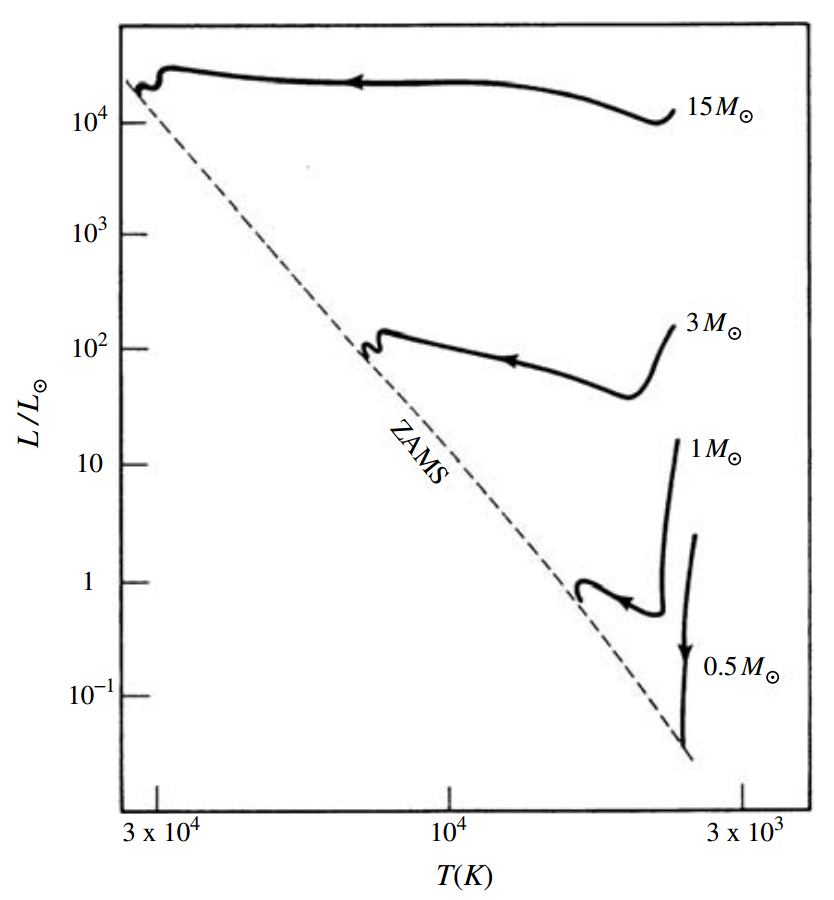
\includegraphics[scale=0.3]{Introduccion/Figures/EvolucionZAMSFormacionEstelar_Kutner.png}
	\caption{Diagrama de la evolución de una protoestrella hasta llegar a
	\textit{ZAMS} (\textit{Zero Age Main Sequence}), la edad a la que se
	convierte en una estrella de secuencia principal. Se muestran varios caminos
	evolutivos de una protoestrella en función de su masa, el cual es el
	parámetro de mayor importancia en su evolución y estado final. Figura
	obtenida de \citetbookchapter{astronomyPhysicalPerspective}{15}.}
	\label{protostarEvolutionFig}
\end{figure}

\subsection{Secuencia Principal}

Una vez que una estrella llegue su etapa de secuencia principal el sistema se
vuelve estable a largas escalas temporales. En este estado la estrella deja de
comprimirse, ya que el colapso gravitacional es contrarrestado por la presión
del gas caliente en su interior y la presión ejercida por la radiación producida
en su núcleo. A continuación se definen dos conceptos importantes en la física
estelar: el \textbf{equilibrio hidrostático} y el \textbf{equilibrio
termodinámico local}.

\subsubsection{Equilibrio Hidrostático}

Podemos simplificar el modelo de una estrella al introducir la simetría
esférica, en el cual las propiedades del gas que forma la estrella dependen
unicamente de la distancia del núcleo. Para esto definimos la presión $P(r)$,
densidad $\rho (r)$, temperatura $T(r)$, y aceleración gravitacional $g(r)$ como
funciones con respecto a la distancia $r$ del centro. En base a estos
fundamentos se puede deducir la estratificación de una estrella, formando varias
capas de material con propiedades uniformes a lo largo de cada estrato. Dado que
cada elemento está sujeto a un equilibrio de fuerzas descrita por la ecuación
$P(r) \mathrm{d}A - [P(r) + \mathrm{d}P] \mathrm{d}A - [\rho(r) \mathrm{d}A
\mathrm{d}r] g(r) = 0$, la cual se ve en la
\reffigure{figuraEquilibrioHidrostatico}. Al simplificar esta ecuación e
introduciendo un término para la presión radiativa\textemdash debido a la
transferencia de momento de los fotones generados en el núcleo estelar al
material circundante\textemdash se obtiene la
\refequation{ecuacionEquilibrioHistrostatico}. 

\begin{eqfloat}[!ht]
	\centering
	\begin{equation}
		\frac{\textrm{d}P(r)}{\textrm{d}r} = -\rho(r) [g(r) - g_{rad}(r)]
	\end{equation}
	\caption{Ecuación del equilibrio hidrostático para una estrella, tomando en
	cuenta los efectos de la presión radiativa saliente $g_{rad}(r)$.
	\citetbookchapter{anIntroStellarAstro}{2}}
	\label{ecuacionEquilibrioHistrostatico}
\end{eqfloat}

\begin{figure}[!ht]
	\centering
	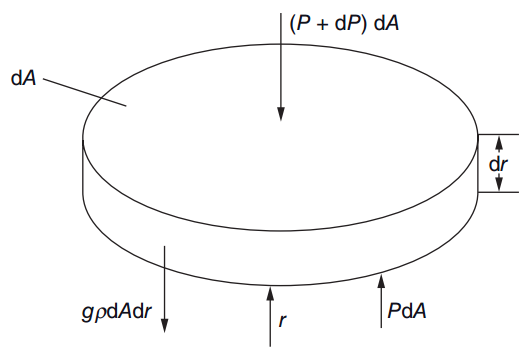
\includegraphics[scale=0.5]{Introduccion/Figures/EquilibrioHidrostatico_LeBlanc.png}
	\caption{Diagrama de fuerzas actuando sobre cada elemento superficial
	$\mathrm{d}A$ de material de una estrella. Los efectos debido a elementos
	adyacentes son nulos, debido a que la presión en cada lados es constante,
	resultando en un gradiente de presión radial. Figura obtenida de
	\citetbookchapter{anIntroStellarAstro}{2}.}
	\label{figuraEquilibrioHidrostatico}
\end{figure}

\subsubsection{Equilibrio Termodinámico Local}

Una estrella como resultado de su mecanismo de transporte de energía no está en
un estado de equilibrio térmico. El núcleo, en donde se produce la gran mayoría
de energía en una estrella, está a ordenes de magnitud más caliente que la
fotosfera. Este transporte de energía ocurre principalmente por medio de
\textit{radiación} y \textit{convección}; la conducción no juega un papel
significativo. Para que una estrella se mantenga estable durante los miles de
millones de años de su vida debe de estar en un tipo de equilibrio, donde cada
estrato su volumen mantenga una composición estable a largas escalas de tiempo,
lo cual implica que el flujo de energía que ingresa a cada capa es igual a la
cantidad de energía que libera a la siguiente capa. Esto lleva a cabo otra
simplificación en el modelo estelar: una estrella la podemos considerar como un
sistema en \textbf{equilibrio termodinámico local}.

Para declarar que un sistema está en equilibrio termodinámico local debemos
considerar el \textbf{camino libre medio} de una partícula en el interior
estelar. Considerando la distancia recorrida por un fotón antes de ser absorbido
o esparcido por otra partícula obtenemos esta medición, la cual dicta la escala
de espacio del transporte de energía comparado a la escala espacial de la
estrella. En el caso de que el camino libre medio sea significativamente menor
que las dimensiones espaciales de la estrella su volumen se puede dividir en
celdas discretas de tamaño despreciable, en las cuales cada una de las celdas
está en equilibrio termodinámico dentro de si mismas
\citetbookchapter{anIntroTheoryStellarStructureEvolution}{2}. Por lo tanto, la
estructura de la estrella se puede determinar siempre y cuando se sepa la masa
de la estrella, y la densidad, temperatura, y composición química de cada punto
en su interior.

\subsection{Evolución}

En el transcurso del tiempo cada estrella será sujeta a ciertos cambios en su
estructura. Esto se debe a que podemos considerar a una estrella cómo un objeto
aislado en el espacio, lo cual significa que no tendrá algún ingreso de material
significativo para reemplazar el combustible \quotes{quemado} en las reacciones
termonucleares. A lo largo del tiempo la composición física y química de la
estrella deberán cambiar para mantener el equilibrio termodinámico.

El combustible primario de una estrella viene siendo el hidrógeno atómico, el
cual se fusiona con otros átomos (protones individuales) libres, resultando en
la producción de grandes cantidades de energía en forma de radiación y moléculas
de helio como producto. El helio no es inmediatamente util para la estrella cómo
combustible, ya que requiere temperaturas más altas de las que se encuentran
durante esta fase evolutiva. Todas las estrellas conocidas pasan por esta etapa
de evolución estelar; mientras que una estrella dependa principalmente del
hidrógeno para brillar se dice que está en su etapa de \textit{secuencia
principal}. 

\begin{figure}[!ht]
	\centering
	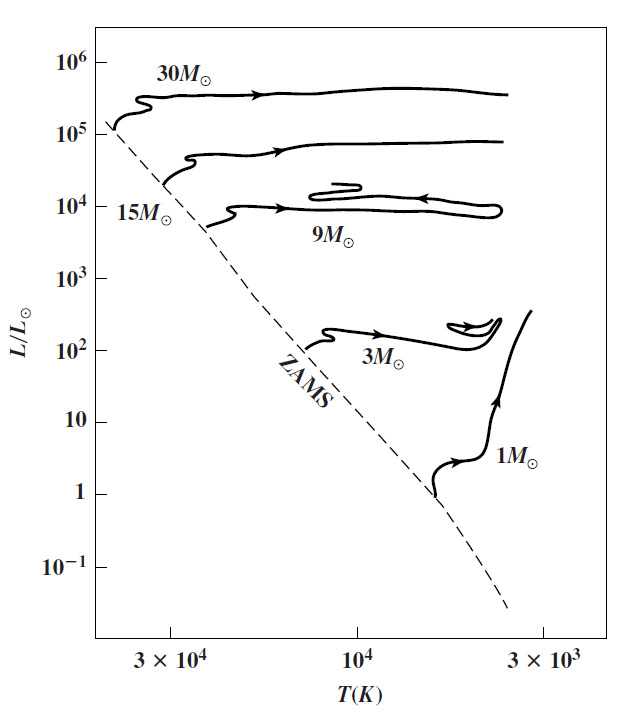
\includegraphics[scale=0.5]{Introduccion/Figures/Figura Evolucion_MS_Astronomy_Physical_Perspective.png}
	\caption{Evolución de estrellas de la secuencia principal basado en su masa
	inicial en el diagrama HR. La línea punteada representa la posición de la
	estrella en el primer momento que se integra a la secuencia principal. Al
	consumir el hidrógeno en su núcleo por las reacciones nucleares que ocurren
	en esta misma región se comienza a desatar el equilibrio delicado que
	mantiene la forma de la estrella. Esta deformación provoca una oscilación en
	su tamaño, causado por las fluctuaciones del balance entre la presión
	radiativa generada por las reacciones nucleares en el núcleo contra la
	presión gravitacional. Diagrama obtenido de
	\citet{astronomyPhysicalPerspective_stellarOldAgeChapter}}
	\label{evolucionMSEstrella}
\end{figure}
% \section{Sistemas Binarios}
\chapter{Sistemas Binarios}

La gran mayoría de sistemas estelares dentro de nuestra Galaxia no son aquellos
solitarios como nuestro propio sistema solar, si no que son compuestas de dos o
más estrellas ubicadas en corta aproximación de una a otra, a ordenes de
unidades astronómicas (AU por sus siglas en inglés). Estos sistemas multiples se
pueden clasificar con mayor precisión para aquellos compuestos de solo dos
estrellas, denominados como \textit{sistemas binarios}. Dentro de un sistema
binario la corta separación orbital entre ambas estrellas da como consecuencia a
fenómenos que surgen mediante la interacción entre las componentes, tanto como
la interacción gravitacional debido a sus masas, como a la física interesante
que ocurre en el caso de interacciones de material entre una estrella a otra. 

Los sistemas binarios estelares ofrecen un laboratorio celeste de gran
importancia, ya que debido a la interacción a cortas escalas espaciales nos
brindan información acerca de las estrellas que sería imposible obtener de otra
manera. \citetbooksection{phoebeScientificReference}{2.1} menciona varios
parámetros derivados de observaciones de estos sistemas, como las masas de cada
una de las componentes estelares por medio de su interacción gravitacional, la
calibración y estudio de la evolución estelar y su dependencia de la masa y
luminosidad de la estrella; dadas observaciones de sistemas desconectados, en el
cual ambas componentes son de la misma edad pero con diferentes propiedades que
influyen su camino evolutivo. La clasificación de estos sistemas se basa tanto
en propiedades observacionales\textemdash las cuales dependen tanto de las
propiedades geométricas del sistema como de nuestra capacidad de observación, en
cuanto a la capacidad de la instrumentación disponible\textemdash como en las
propiedades físicas del sistema, incluyendo la proximidad de las componentes
como sus propiedades lumínica.

\section{Geometría del Sistema - Modelo de Roche}

Es importante entender la forma geométrica de un sistema binario para llegar a
una descripción adecuada de ellos. Esto incluye los parámetros orbitales de las
estrellas tanto como la forma misma de ambas componentes, ya que en ciertos
casos tratar las estrellas como esferas rígidas da como resultado un modelo
incorrecto. A continuación se introduce las bases de las cuales se parte para
llegar a una representación de un sistema modelo, llegando a describir el
\textbf{modelo de Roche}.

Se define un sistema de coordenadas cartesiano tridimensional considerando un
marco de referencia no inercial, el cual está rotando con la misma velocidad que
las componentes del sistema binario orbitan una a otra. Esta es una
representación típica para el \textit{problema de tres cuerpos}, en el cual
tenemos a dos objetos masivos cuya influencia gravitacional se extiende al
espacio representado por el sistema de coordenadas. En la
\reffigure{figuraTresCuerpos} se puede ver este esquema, donde $m_1$ y $m_2$
representan ambas componentes estelares, posicionadas de tal manera que la
distancia entre las estrellas solo tenga una componente en una dirección
cartesiana.

\begin{figure}[!ht]
	\centering
	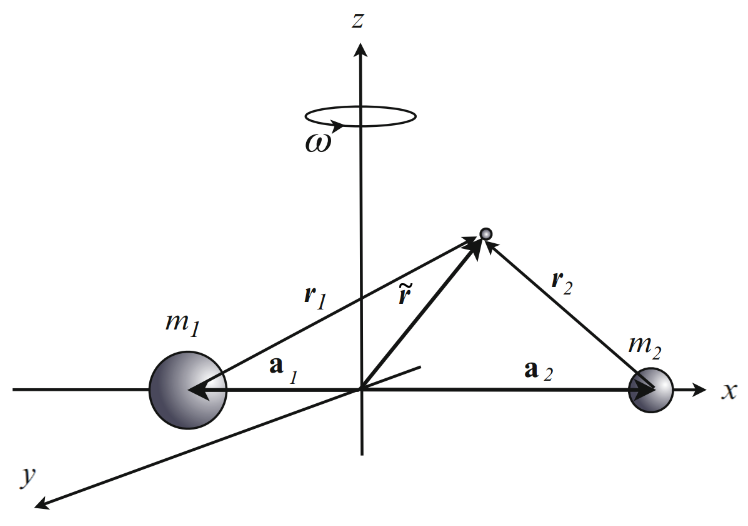
\includegraphics[scale=0.6]{Introduccion/Figures/Figura Tres Cuerpos_Intro Evolution Single Binary Stars.png}
	\caption{Configuración del problema de tres cuerpos dados dos objetos de
	alta masa $m_1$ y $m_2$ (las cuales representan cada componente estelar del
	sistema binario), y una partícula de masa despreciable de prueba ubicada a
	una distancia $r_1$ y $r_2$ de las estrellas respectivamente. El centro de
	masa del sistema está ubicado en el origen del sistema de coordenadas.
	Figura obtenida de
	\citetbooksection{benacquista_introduction_to_evolution_single_binary_stars_2013}{13.1},
	modificada cambiando los ejes $y$ y $x$ para que $m_1$ y $m_2$ estén
	ubicadas en el eje $x$ para ser consistente con
	\citetbooksection{phoebeScientificReference}{3.1}.}
	\label{figuraTresCuerpos}
\end{figure}

La \reffigure{figuraTresCuerpos} define el sistema de coordenadas rotando junto
al sistema binario. La velocidad angular de Kepler está dada por:

\begin{eqfloat}[!ht]
	\centering
	\begin{equation}
		\omega = \frac{2 \pi}{P_{orb}} = \sqrt{\frac{G (m_1 + m_2)}{a^3}}
	\end{equation}
	\blankcaption
	\label{ecuacionVelocidadAngular}
\end{eqfloat}

Donde $G = 6.673 \times 10^{-11} \ \mathrm{m}^3 \mathrm{kg}^{-1}
\mathrm{s}^{-2}$ es la constante de gravitación universal, $P_{orb}$ es el
periodo orbital de las estrellas (el cual es igual para ambas estrellas de
acuerdo a la segunda ley de Kepler), y $a = a_1 + a_2$ es el semieje mayor.
Usando la \refequation{ecuacionVelocidadAngular} podemos definir el Lagrangiano
para una partícula de prueba con masa $m$, el cual está a una distancia
$\mathbf{r}_1$ y $\mathbf{r}_2$ de $m_1$ y $m_2$ respectivamente:

\begin{eqfloat}[!ht]
	\centering
	\vspace{1em}
	\begin{equation}
		\Lagr = \eqnmark[MyDarkRed]{node1}{\frac{1}{2} m (\dot{x}^2 + \dot{y}^2 + \dot{z}^2)} +
				\eqnmark[MyDarkGreen]{node2}{\frac{1}{2} m \omega^2 \tilde{r}^2} +
				\eqnmark[MyDarkBlue]{node3}{\frac{G m_1 m}{r_1} + \frac{G m_2 m}{r_2}}
	\end{equation}
	\annotate[yshift=-0.2em]{below, left}{node1}{Energía cinética lineal}
	\annotate[yshift=0.75em]{above, left}{node2}{Energía cinética rotacional}
	\annotate[yshift=-0.75em]{below, left}{node3}{Potencial gravitacional}
	\blankcaption
	\vspace{0.4em}
	\label{ecuacionLagrangianoTresCuerpos}
\end{eqfloat}

Donde $\tilde{r}$ es la distancia al eje de rotación del marco de referencia,
$r_1 = \abs{\mathbf{r}_1} = \abs{\mathbf{r} - \mathbf{a}_1}$ y $r_2 =
\abs{\mathbf{r}_2} = \abs{\mathbf{r} - \mathbf{a}_2}$. Utilizando los últimos 3
términos de la \refequation{ecuacionLagrangianoTresCuerpos} podemos definir un
pseudo-potencial que determina el movimiento de la partícula de prueba, tanto
por la influencia gravitacional de las componentes como la fuerza centrifugal
dada por la rotación del marco de referencia. Esta ecuación se puede simplificar
al colocar el origen del sistema sobre la masa $m_1$ en vez de su centro de
masa, donde $x_{1} = 0$ es la posición de $m_1$ y $x_2 = \mathbf{a}_1 +
\mathbf{a}_2 = \mathbf{a}$ es la posición de la secundaria. Por lo tanto, la
nueva coordenada del centro de masa del sistema se da por:

\begin{eqfloat}[!ht]
	\centering
	\begin{equation}
		x_{\textrm{CoM}} = \frac{\sum_{i}{m_i x_i}}{\sum_{i}{m_i}} = \frac{qa}{1 + q}
	\end{equation}
	\blankcaption
	\label{ecuacionCentroDeMasa}
\end{eqfloat}

Donde se introduce el parámetro para la razón de masa $q = \frac{m_2}{m_1}$. En
varios trabajos las componentes de un sistema binario son identificados de tal
manera que $q \leq 1$; sin embargo, esta convención no suele ser conveniente al
momento de crear un modelo del sistema (por ejemplo,
\citeyearparen{ding_fast_derivation_cbs_params_2022}), en donde se permite que $q >
1$ al asignar la componente primaria basado en parámetros orbitales en vez de
sus masas.

Este potencial efectivo $\psi$ se obtiene asumiendo una distribución de masa
esférica para ambas estrellas \citetbooksection{phoebeScientificReference}{3.1}:

\begin{eqfloat}[!ht]
	\centering
	\begin{equation}
		\psi = -\frac{G m_1}{r_1} - \frac{G m_2}{r_2} - \frac{1}{2} \omega \tilde{r}^2
	\end{equation}
	\blankcaption
	\label{ecuacionPotencialEfectivo}
\end{eqfloat}

Usando el potencial $\psi$ es posible llegar a un potencial adimensional
$\Omega$ el cual determina la forma de ambas componentes. La geometría del
sistema se presta a un sistema de coordenadas esféricas, usando un ángulo polar
$\theta$ cuyo valor va desde $0$ en polo norte hasta $180^{\circ}$ en el polo
sur\textemdash paralelo al eje $z$ en la
\reffigure{figuraTresCuerpos}\textemdash y un ángulo azimutal $\phi$ cuyo valor
es $0$ en el eje $x$. Utilizamos las siguientes expresiones para convertir de
coordenadas cartesianas a coordenadas esféricas:

\begin{eqfloat}[!ht]
	\centering
	\begin{equation}
		\begin{split}
			& x = r \sin{\theta} \cos{\phi} = \lambda r \\
			& y = r \sin{\theta} \sin{\phi} = \mu r \\
			& z = r \cos{\theta} = \nu r
		\end{split}
	\end{equation}
	\blankcaption
	\label{ecuacionesCoordsEsfericasConversion}
\end{eqfloat}

En donde $r = \sqrt{x^2 + y^2 + z^2}$ es la distancia entre la partícula de
prueba ubicada en el punto $(x, y, z)$ al origen del sistema de coordenadas.
Partiendo del teorema de Pitágoras se puede llegar a una ecuación para calcular
la distancia $D$ entre dos puntos ubicados en $(x, y, z)$ y $(x', y', z')$ en un
sistema de coordenadas esférico:

\begin{eqfloat}[!ht]
	\centering
	\begin{equation}
		D = \sqrt{(x - x')^2 + (y - y')^2 + (z - z')^2}
	\end{equation}
\end{eqfloat}

La cual al expandir obtenemos:

\begin{eqfloat}[!ht]
	\centering
	\begin{equation}
		D = \sqrt{x^2 - 2xx' + x'^2 + y^2 - 2yy' + y'^2 + z^2 - 2zz' + z'^2}
		% D = \sqrt{\eqnmark[MyDarkBlue]{rNode1}{x^2} - 2xx' + x'^2 + \eqnmark[MyDarkBlue]{rNode2}{y^2} - 2yy' + y'^2 + \eqnmark[MyDarkBlue]{rNode3}{z^2} - 2zz' + z'^2}
	\end{equation}
\end{eqfloat}

Sustituyendo usando $d_1 = \sqrt{x^2 + y^2 + z^2}$ y $d_2 = \sqrt{x'^2 + y'^2 +
z'^2}$ como las distancias de ambos puntos al origen se obtiene:

\begin{eqfloat}[!ht]
	\centering
	\begin{equation}
		D = \sqrt{d_1^2 + d_2^2 - 2xx' - 2yy' -2zz'}
	\end{equation}
	\blankcaption
	\label{ecuacionDistanciaCartesiana}
\end{eqfloat}

Para obtener la distancia $D$ en coordenadas esféricas es necesario hacer la
conversión utilizando las \refequations{ecuacionesCoordsEsfericasConversion}, llegando a la expresión final:

\begin{eqfloat}[!ht]
	\centering
	\begin{equation}
		D = \sqrt{d_1^2 + d_2^2 - 2d_1d_2[(\sin{\theta} \sin{\theta'})(\cos{\phi - \phi'}) + \cos{\theta} \cos{\theta'}]}
	\end{equation}
	\blankcaption
	\label{ecuacionDistanciasEsferica}
\end{eqfloat}

Donde los puntos $(x, y, z)$ y $(x', y', z')$ corresponden a $(d_1, \theta,
\phi)$ y $(d_2, \theta', \phi')$ respectivamente. Se puede utilizar la
\refequation{ecuacionDistanciaCartesiana} y
\refequation{ecuacionDistanciasEsferica}\textemdash y haciendo uso de las
\refequations{ecuacionesCoordsEsfericasConversion}\textemdash para obtener las
distancias de la partícula de prueba $m$ a ambas componentes estelares del
sistema:

\begin{eqfloat}
	\centering
	\begin{equation}
		\begin{split}
			& r_1 = r \\
			& r_2 = \sqrt{r^2 - 2ax + a^2} = \sqrt{r^2 - 2ar\lambda + a^2} \\
			& \tilde{r} = \sqrt{(x - x_{\textrm{CoM}})^2 + y^2} = \sqrt{r^2(1 - \nu^2) - 2r\lambda x_{\textrm{CoM}} + x_{\textrm{CoM}}^2}
		\end{split}
	\end{equation}
	\blankcaption
	\label{ecuacionesDistancias}
\end{eqfloat}

Notando que el origen del sistema de coordenadas está ubicada en la posición de
la componente $m_1$. Por lo tanto, el potencial es definido con respecto a
$m_1$; para obtener el potencial con respecto a $m_2$ es necesario hacer una
transformación descrita en \citetbooksection{phoebeScientificReference}{3.1}.
Sustituyendo las ecuaciones \refequations{ecuacionesDistancias} en la expresión
del potencial $\psi$ se obtiene el potencial efectivo en coordenadas esféricas:

\begin{eqfloat}[!ht]
	\centering
	\begin{equation}
		\psi(r, \lambda, \nu) = -\frac{Gm_1}{r} - \frac{Gm_2}{\sqrt{r^2 - 2ar\lambda + a^2}} - \frac{1}{2} \omega^2 (r^2(1-\nu^2) - 2r\lambda x_{\textrm{CoM}} + x_{\textrm{CoM}}^2)
	\end{equation}
	\blankcaption
	\label{ecuacionPotencialEfectivoEsferico}
\end{eqfloat}

Utilizando la tercera ley de Kepler de la forma $\omega^2 a^3 = G(m_1 + m_2)$
junto a la \refequation{ecuacionCentroDeMasa} y sustituyendo en la
\refequation{ecuacionPotencialEfectivoEsferico} se obtiene la forma final del
potencial efectivo, eliminando la dependencia explicita a la velocidad angular
del sistema y de la masa de la secundaria $m_2$
\citetbooksection{phoebeScientificReference}{3.1}:

\begin{eqfloat}[!ht]
	\centering
	\begin{equation}
		\begin{split}
			\psi(r, \lambda, \nu) = -\frac{G m_1}{a} \left[ \frac{a}{r} + q \left(\frac{a}{\sqrt{r^2 - 2ar\lambda + a^2}} - \frac{r\lambda}{a} \right) \right.\\
			\left. + \frac{r^2}{2a^2}(1 + q)(1 - \nu^2) + \frac{q}{2(1 + q)} \right]
		\end{split}
	\end{equation}
	\blankcaption
	\label{ecuacionPotencialEfectivoFinal}
\end{eqfloat}

El potencial efectivo en la \refequation{ecuacionPotencialEfectivoFinal} se puede utilizar para definir un potencial adimensional, el cual define la forma de ambas componentes. Este potencial $\Omega$ se refiere al \textbf{potencial modificado de Kopal}, introducido en \citetbookchapter{kopal_close_binary_systems_1959}{III.1}. Este potencial se relaciona con $\psi$ por la siguiente ecuación:

\begin{eqfloat}[!ht]
	\centering
	\begin{equation}
		\Omega = -\frac{a \psi}{G m_1} - \frac{m_2^2}{2m_1(m_1 + m_2)}
	\end{equation}
\end{eqfloat}

El segundo término del RHS se puede simplificar multiplicando por $\frac{1/m_1^2}{1/m_1^2}$:

\begin{eqfloat}[!ht]
	\centering
	\begin{equation}
		\Omega = -\frac{a \psi}{G m_1} - \frac{q^2}{2(1 + q)}
	\end{equation}
	\blankcaption
	\label{ecuacionRochePotencialEfectivo}
\end{eqfloat}

Sustituyendo la \refequation{ecuacionPotencialEfectivoFinal} en
\refequation{ecuacionRochePotencialEfectivo} obtenemos obtenemos el potencial modificado
de Kopal:

\begin{eqfloat}[!ht]
	\centering
	\begin{equation}
		\Omega = \frac{1}{\varrho} + q\left(\frac{1}{\sqrt{\varrho^2 - 2\varrho \lambda + 1}} - \varrho \lambda \right) + \frac{1}{2} (1 + q)(1 - \nu^2)\varrho^2
	\end{equation}
	\blankcaption
	\label{ecuacionRoche}
\end{eqfloat}

Introduciendo la variable adimensional $\varrho = \frac{r}{a}$ usada en
\citetbooksection{phoebeScientificReference}{3.1}. Usando la
\refequation{ecuacionRoche} podemos determinar la forma de ambas estrellas
asumiendo que la envoltura estelar (es decir, la capa superficial) coincide con
superficies de \textbf{equipotenciales de Roche}, donde el valor de $\Omega$ es
constante en toda la superficie
\citetbookchapter{kopal_close_binary_systems_1959}{3}. Este modelo de las
superficies estelares de un sistema binario comparte el nombre con el originador
de esta idea, el matemático francés \textit{Édouard Albert Roche} del siglo XIX.
Sin embargo, para que este modelo sea una buena aproximación del fenómeno
astrofísico debe de cumplir con las siguientes condiciones:

\begin{description}
	\item[Órbita circular sincrónica -] La formalización de los equipotenciales
	de Roche presentado en esta sección solo aplica para sistemas binarios cuya
	órbita es circular y sincrónica (los periodos de rotación de ambas estrellas
	son iguales al periodo orbital). 
	
	\item[Oscilaciones no-radiales despreciables -]  Las estrellas por
	imbalances locales padecen de una distorsión anisótropo, el cual causa que
	la superficie estelar se desvíe del modelo de Roche. Sin embargo, en la
	mayoría de las estrellas estas oscilaciones no-radiales ocurren en el orden
	de la escala de tiempo hidrostática, la cual, por ejemplo, es de ~15 minutos
	para una estrella tipo solar
	\citetbooksection{kallrath_eclipsing_binary_modelling_2009}{3.1.5}. Mientras
	la escala de tiempo de estas distorsiones sea despreciable con respecto al
	periodo orbital la superficie estelar (su fotósfera) se puede parametrizar
	con el modelo de Roche.

	\item[Alta densidad de masa -] A pesar de que el material de una estrella
	esté distribuido por todo su volumen, el modelo de Roche simplifica la
	composición de una estrella a un punto infinitesimal el cual ejerce una
	fuerza gravitacional alrededor. Esta aproximación resulta en una superficie
	sin masa, cuya forma es dictada por el potencial de Roche. Esta aproximación
	permite derivar la expresión analítica en la \refequation{ecuacionRoche}, la
	cual se puede aplicar a fenómenos de alta \quotes{condensación central}
	\citetbookchapter{kopal_close_binary_systems_1959}{III}.
\end{description}

\subsection{Generalización a Órbitas Excéntricas y Asincrónicas}

% TODO: porqué no se puede modelar 
Una desventaja del modelo de Roche presentado en la \refequation{ecuacionRoche}
yace en sus suposiciones principales; como consecuencia de estas, el potencial
$\Omega$ definido hasta ahora solo puede ser aplicado a aquellos sistemas
binarios cuya órbita es circular y sincrónica. Esto excluye los sistemas con
órbitas excéntricas y/o asincrónicas, incluyendo sistemas binarios en contacto
cuyas propiedades no pueden ser adecuadamente modeladas en este paradigma
\citetbooksection{kallrath_eclipsing_binary_modelling_2009}{3.1.5}.
\citeyearparen{wilson_eccentric_1979} generaliza el modelo de Roche a este tipo de
órbitas, llegando a la siguiente expresión:

\begin{eqfloat}[!ht]
	\centering
	\begin{equation}
		\Omega = \frac{1}{\varrho} + q \left(\frac{1}{\sqrt{\delta^2 + \varrho^2 - 2\varrho \delta \lambda}} - \frac{\varrho \lambda}{\delta^2} \right) + \frac{F^2 \varrho^2 (1 + q)(1 - \nu^2)}{2}
	\end{equation}
	\blankcaption
	\label{ecuacionRocheExcentricaAsincronica}
\end{eqfloat}

Introduciendo dos términos: el \textit{parámetro de sincronicidad} $F =
\omega_{\mathrm{rot}} / \omega_{\mathrm{orb}}$ la razón de la velocidad angular rotacional de la
componente a su velocidad angular orbital, y la \textit{separación instantánea}
entre ambas componentes $\delta = D / a$ normalizada con respecto al semieje
mayor $a$ \citetbooksection{phoebeScientificReference}{3.1}. El cambio principal
de este potencial modificado se refleja en la dependencia en la fase orbital del
campo potencial; debido a la excentricidad del sistema, las componentes no
mantienen una distancia constante una de otra, por lo cual el potencial de de
ser nuevamente calculado para cada fase. Al igual, este modelo considera
aquellos casos donde $F \neq 1$, ignorando los efectos de rotación diferencial
en las estrellas por simplicidad. Para el caso de una órbita sincrónica y
circular (es decir, $F = 1$ y $D = a$) la
\refequation{ecuacionRocheExcentricaAsincronica} se reduce a la
\refequation{ecuacionRoche}. Partiendo de esta ecuación se puede determinar la
forma de ambas estrellas.

\subsection{Superficies Equipotenciales}

La forma de una estrella en el modelo de Roche es determinada por una
\textbf{superficie equipotencial}, en la cual el valor del potencial $\Omega$ es
igual, identificado por un contorno. Una forma conveniente de definir la
superficie de un sistema es dando el valor de $\Omega$ en el polo norte de la
estrella primaria, en las coordenadas polares $(\theta = 0 \rightarrow \lambda = 0,\nu =
1)$; partiendo de este valor, incluyendo otros parámetros del sistema como la
razón de masa y el semieje mayor de la órbita, se define el contorno para el
valor del potencial del polo, denominado como $\Omega_{\mathrm{pol}}$. La
expresión para el potencial del polo se reduce a:

\begin{eqfloat}[!ht]
	\centering
	\begin{equation}
		\Omega_{\textrm{pol}} = \frac{1}{\varrho_{\textrm{pol}}} + \frac{q}{\sqrt{\delta^2 + \varrho_{\textrm{pol}}}}
	\end{equation}
	\blankcaption
	\label{ecuacionPotencialPoloRadio}
\end{eqfloat}

Donde $\Omega_{\textrm{pol}}$ es el valor del potencial modificado de Roche en
el polo de la estrella, y $\varrho_{\textrm{pol}}$ es el radio normalizado al
semieje mayor en el polo de la estrella. Usando esta expresión se puede
parametrizar la forma y tamaño de la estrella utilizando un solo valor para el
potencial; esto es gracias a la siguiente relación dada en
\citetbooksection{phoebeScientificReference}{3.1}:

\begin{eqfloat}[!ht]
	\centering
	\begin{equation}
		\nabla p \parallel \rho \parallel \psi
	\end{equation}
\end{eqfloat}

% TODO: newpage para mantener formato de documento
\newpage

Esta nos dice que el gradiente de la densidad $\rho$, la presión $p$, y el
potencial efectivo $\psi$ son paralelo uno a otro, lo cual necesariamente
implica que una superficie constante del potencial coincide con las superficies
constantes de densidad y presión. Esta superficie equipotencial es resuelta
utilizando la \refequation{ecuacionPotencialPoloRadio} y
\refequation{ecuacionRocheExcentricaAsincronica}, dando el valor $\Omega =
\Omega_{\textrm{pol}}$ del sistema:

\begin{eqfloat}[!ht]
	\centering
	\begin{equation}
		\frac{1}{\varrho_{\textrm{pol}}} + \frac{q}{\sqrt{\delta^2 + \varrho_{\textrm{pol}}}} = \frac{1}{\varrho} + q \left(\frac{1}{\sqrt{\delta^2 + \varrho^2 - 2\varrho \delta \lambda}} - \frac{\varrho \lambda}{\delta^2} \right) + \frac{F^2 \varrho^2 (1 + q)(1 - \nu^2)}{2}
	\end{equation}
	\blankcaption
	\label{ecuacionRadioPolarEstelarEquivalencia}
\end{eqfloat}

Esta es resuelta de manera iterativa para cada valor de $\lambda$ y $\nu$ de la
malla de valores utilizada en el problema. El resultado es la forma de ambas
componentes del sistema binario, las cuales ya no son unas simples esferas o
incluso elipses, si no que toman una forma de gota que sigue el campo de
potencial establecido por medio de las fuerzas que rigen el sistema:

\begin{figure}[!ht]
	\centering
	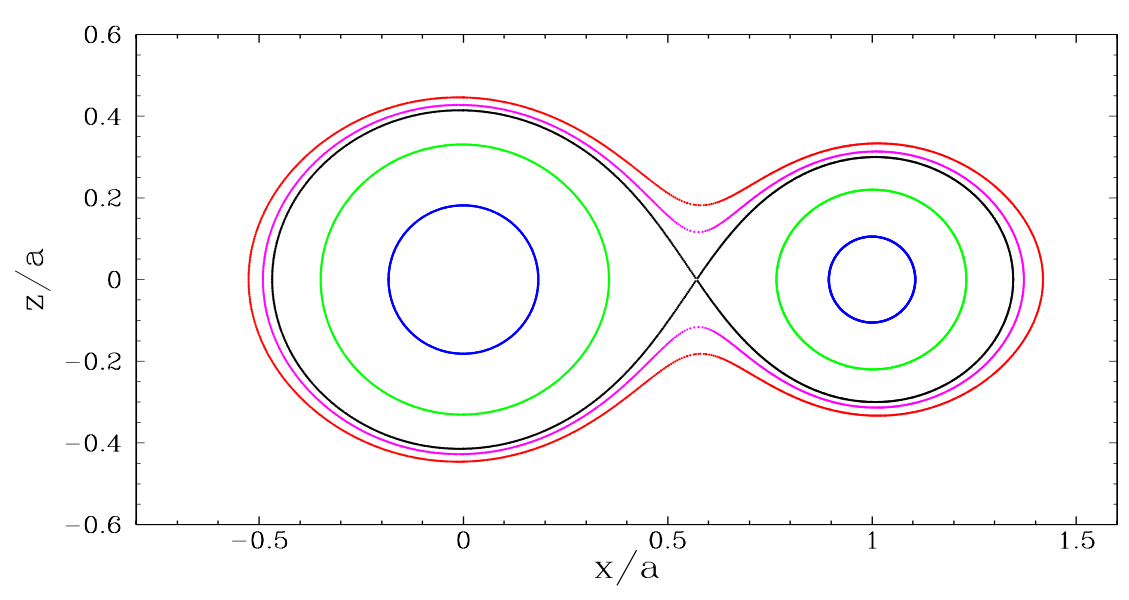
\includegraphics[scale=0.4]{Introduccion/Figures/Figura Forma Roche_PHOEBE Reference.png}
	\caption{Distintas formas de las componentes dependiendo del valor dado para $\Omega$. El potencial azul corresponde a $\Omega = 6.0$, verde a $\Omega = 3.5$, magenta a $\Omega = 2.8$, y rojo a $\Omega = 2.7$. La superficie negra corresponde a $\Omega = 2.87584$, el cual se le conoce como el \textbf{lóbulo de Roche crítico}. Figura obtenida de \citetbooksection{phoebeScientificReference}{3.1}.}
	\label{figuraRocheFormaPhoebe}
\end{figure}

\section{Clasificación Morfológica}

Debido a que la estructura del potencial de Roche es una de las propiedades más
importantes para un sistema binario estelar, se acostumbran a clasificar en base
a la forma del potencial. Como se puede ver en la
\reffigure{figuraRocheFormaPhoebe}, diferentes valores para el potencial polar
$\Omega_{\mathrm{pol}}$ deforma ambas estrellas de maneras distintas, empezando
con componentes mayormente esféricas para altos valores de $\Omega$, hasta
llegar a sistemas en contacto en el caso de $\Omega < 2.87584$; la importancia
de este valor es explicada en esta sección.

\subsection{Sistemas Separados}

Los \textbf{sistemas separados} son aquellos cuya distancia orbital es
suficientemente grande para que las componentes estelares no hagan contacto
físico una con otra. Por lo tanto, estas componentes interactúan entre si
principalmente mediante sus campos gravitacionales, distorsionando la forma de
su compañera estelar. Las superficies estelares pueden ser mayormente esféricas
o elipsoidales dependiendo del campo de potencial, como se puede ver en la
\reffigure{figuraRocheFormaPhoebe} para los modelos que corresponden a $\Omega =
6.0$ y $\Omega = 3.5$. Estos sistemas son laboratorios importantes en el estudio
de las propiedades físicas de las estrellas, debido ńo solo a que permiten
calcular sus masas por medio de su interacción gravitacional, pero el hecho que
no tengan contacto físico permite estudiar las propiedades evolutivas de las
estrellas, ya que ambas componentes se desarrollan de manera independiente.

\subsection{Sistemas Semi-separados}

Un \textbf{sistema semi-separado} se distingue de otras morfologías debido a que
la separación orbital de las componentes estelares llega a ser del orden de
magnitud de unos cuantos radios solares. Esto causa que las superficies
equipotenciales de ambas estrellas se acerquen una a otra. En la
\reffigure{figuraRocheFormaPhoebe} se puede ver destacada la superficie de color
negro, en el cual el potencial de una componente está en contacto con su
compañera. Esta superficie se le conoce como el \textbf{lóbulo de Roche
crítico}, o simplemente como el \textbf{lóbulo de Roche}. El punto en el que
están en contacto es una región del espacio particular al problema de tres
cuerpos, que se le conoce como un \textit{punto de Lagrange}. Estas regiones del
espacio dentro del marco de referencia no-inercial marcan donde las fuerzas
ejercidas por el campo potencial de las componentes es igual a 0; una partícula
dentro de una de estas regiones no es sometida a ninguna aceleración. La
\reffigure{figuraLagrange} muestra las posiciones relativas de los puntos de
Lagrange.

\begin{figure}[!ht]
	\centering
	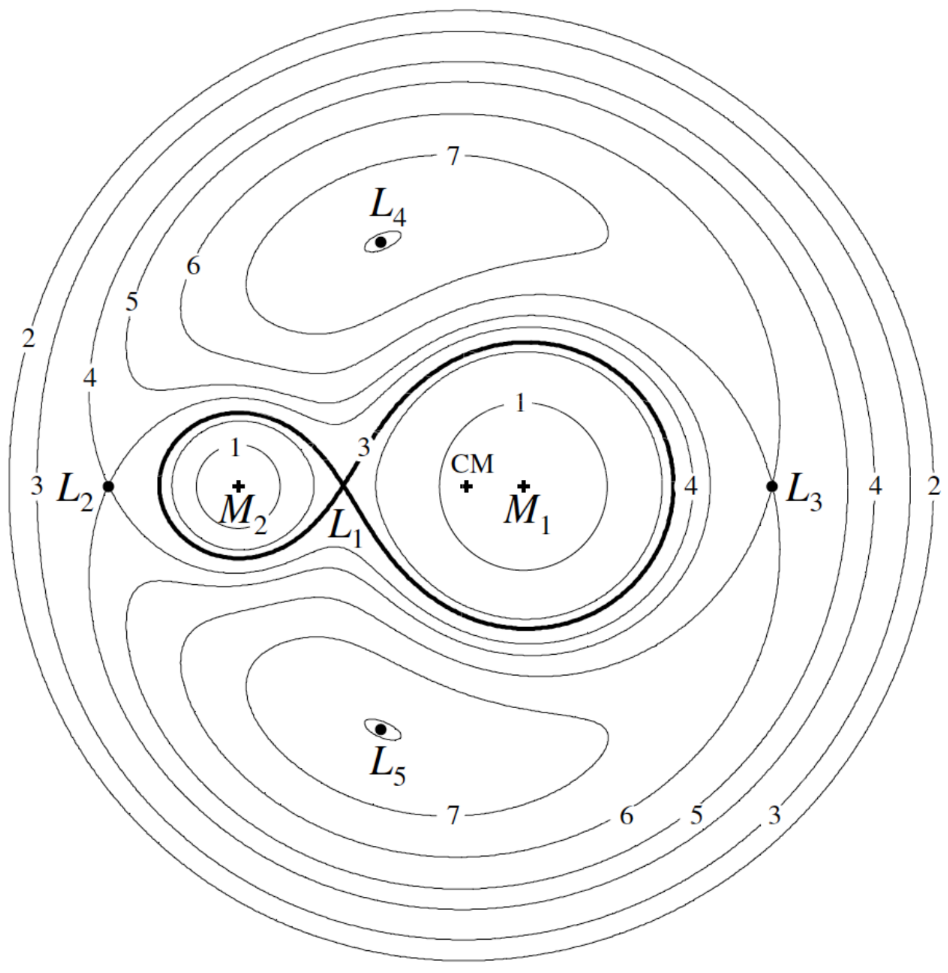
\includegraphics[scale=0.34]{Introduccion/Figures/Figura Lagrange_CVs Wide Field Surveys.png}
	\caption{El modelo de Roche para un sistema binario con una razón de masa $q
	= m_2 / m_1 = 0.25$. Se pueden apreciar los cinco puntos de
	Lagrange\textemdash \textit{L1}- \textit{L5}\textemdash que resultan del
	campo del potencial $\Omega$. Figura obtenida de
	\citeyearparen{ibanez_cvs_wide_field_surveys_2021}.}
	\label{figuraLagrange}
\end{figure}

De interés particular es el punto \textit{L1}, el punto de contacto entre ambas
componentes. Una vez que una componente llene su lóbulo de Roche, el material
que previamente estaba ligado a su superficie será atraída gravitacionalmente a
la compañera estelar, iniciando un proceso de acreción de material. Las
\textit{variables cataclísmicas} son un ejemplo de este tipo de sistemas
binarios semi-separados, donde la componente secundaria enana roja llena su
lóbulo de Roche, transfiriendo material a la componente primaria enana blanca.

\subsection{Sistemas en Contacto}

Un sistema con un valor suficientemente pequeño de su potencial de Roche es un
\textbf{sistema binario en contacto}. A diferencia de un sistema semi-separado,
ambas componentes llenan su lóbulo de Roche en un sistema en contacto, haciendo
contacto en el punto de Lagrange \textit{L1}. Este caso de contacto (también
llamado un sistema en \textit{sobre-contacto} debido a que las estrellas no solo
están en contacto con su lóbulo de Roche, si no que su material se derrama fuera
del lóbulo crítico) da origen al fenómeno de una \textbf{envoltura común}: esta
es una superficie equipotencial que envuelve a ambas estrellas, en lugar de que
cada componente tenga su propia fotósfera independiente. La región de
conexión\textemdash conocida como el \quotes{cuello} del sistema por su nombre
en inglés\textemdash actúa como un puente entre las dos estrellas, sirviendo
como un medio de transporte de tanto material estelar como energía. Ejemplos de
superficies equipotenciales para estos sistemas se pueden ver en la
\reffigure{figuraRocheFormaPhoebe}, las cuales corresponden a $\Omega = 2.8$ y
$\Omega = 2.7$.

En el estudio de sistemas en contacto es importante introducir un nuevo
parámetro el cual describe la cantidad en que el sistema está en sobre-contacto.
El \textbf{factor de relleno}, por su nombre en inglés \textbf{fillout factor},
se define por medio de los valores del potencial en los puntos de Lagrange $L1
\rightarrow \Omega^{L1}_{\mathrm{crit}}$ y $L2 \rightarrow
\Omega^{L2}_{\mathrm{crit}}$:

\begin{eqfloat}
	\centering
	\begin{equation}
		\mathcal{F} = \frac{\Omega - \Omega^{L1}_{\textrm{crit}}}{\Omega^{L2}_{\textrm{crit}} - \Omega^{L1}_{\textrm{crit}}}
	\end{equation}
\end{eqfloat}

Esta ecuación describe la concentración espacial del material superficial de las
estrellas, definido unicamente con el potencial efectivo del sistema. El valor
del factor de relleno está restringido los siguientes valores: $\mathcal{F} < 0$
para sistemas separados, $\mathcal{F} = 0$ para el caso de semi-contacto, y $0 <
\mathcal{F} \leq 1$ para el caso de sobre-contacto. El factor de relleno resulta
ser una parametrización util al momento de modelar un sistema en contacto (por
ejemplo, utilizando el paquete de software \textit{PHOEBE}), debido a la
precisión computacional que sería necesaria para ajustar los radios individuales
de las estrellas. 

\section{Clasificaciones Observacionales}

Dependiendo del método de detección y las propiedades aparentes del sistema se
puede clasificar un sistema binario de estrellas. Estas clasificaciones son
independiente de sus propiedades físicas, como la clase espectral de cada
estrella o sus masas individuales. Al determinar su clasificación observacional
se puede delimitar las técnicas observacionales que son viables para recabar
datos del sistema; un sistema astrométrico sería indistinguible de uno
espectroscópico si uno intenta identificar las componentes individuales a simple
vista, o con un telescopio demasiado débil para el trabajo.

\begin{description}
	\item[Binarias visuales -] aquellos sistemas cuya separación orbital
	aparente es suficientemente grande para distinguir las dos estrellas
	individuales en la bóveda celeste. A pesar de que se puede trazar la órbita
	de la secundaria con varios años de observaciones, se requiere de cálculos
	adicionales para determinar la órbita exacta de las componentes. Esto se
	debe a la inclinación del sistema con respecto al eje de observación hacia
	la Tierra; solo es posible observar \quotes{una proyección del elipse
	orbital relativo en el plano del cielo,} aunque esto se puede superar usando
	el hecho de que la estrella primaria aparentemente inmóvil debe de estar
	presente \quotes{en un punto focal de la órbita relativa.}
	\citetbookchapter{fundamentalAstronomy}{10}

	\item[Binarias espectroscópicas -] presentan variaciones periódicas en sus
	espectros, en donde las líneas espectrales detectadas \quotes{oscilan
	periodicamente alrededor de la longitud de onda promedio}
	\citetbookchapter{astronomyPhysicalPerspective}{5}. Esto se observa debido
	al \textit{desplazamiento de Doppler}, lo cual causa que la frecuencia de un
	fotón se recorra hacia frecuencias más pequeñas (azules) o más grandes
	(rojas) dependiendo de su velocidad radial con respecto al observador, si se
	va acercando o alejando, respectivamente. Estas también pueden ser identificadas
	al observar dos distintos grupos de líneas espectrales, el cual es resultado
	de la contribución de ambas estrellas.

	\item[Binarias astrométricas -] al igual que las espectroscópicas, las
	binarias astrométricas solo muestran una componente visible al ser
	observada, al contrario de las binarias visibles. Sin embargo, una binaria
	astrométrica difiera de las otras dos categorías definidas en cuestión de su
	movimiento observado en la bóveda celeste. Estas muestran un movimiento
	errático y no-lineal, algo que no se esperaría ver en una estrella solitaria
	dado su inercia según la primera ley de Newton. Estas perturbaciones son
	causadas por una estrella secundaria no aparente al observar el sistema. 
\end{description}

\section{Binarias Eclipsantes}

Una de las propiedades más útiles de identificar de un sistema binario es
la \textit{inclinación} de su órbita con respecto a la línea de visión
del sitio de observación (ya sea la Tierra en caso de un observatorio
terrestre o un punto lejano dentro del sistema solar para un telescopio
espacial). En dado caso que un sistema tenga una inclinación suficientemente
alta se pueden observar eclipses dentro del sistema, en lo que una componente
obscurece a su compañera de nuestra línea de visión, otorgando el nombre de 
\textbf{binaria eclipsante} a los sistemas que muestran este fenómeno. 
Aparte de su clasificación morfológica física, los sistemas binarios eclipsantes
se pueden distinguir en 3 diferentes tipos de sistemas binarios cercanos,
basados en la forma de su curva de luz.

\subsection{EA - Algol}

Las curvas de luz de tipo \textit{EA} son atribuidas generalmente a sistemas
binarios separados, donde ambas componentes estelares pueden mantener su forma
esférica sin perturbaciones a escalas apreciables. Gracias a esta separación de
las estrellas es posible definir claramente el comienzo y fin de ambos eclipses;
fuera de los eclipses, la curva de luz se mantiene relativamente constante,
mostrando variabilidad despreciable en casos de variabilidad elipsoidal (en el
caso que las componentes no sean esferas perfectas debido a una leve distorsión
por el potencial gravitacional) o en caso del calentamiento superficial de una
componente por la radiación incidente de su compañera
\citeyearparen{samus_gcvs_variable_types_2016}. Existen sistemas con un rango amplio
de periodos orbitales, desde 4 horas hasta más de 25 años. Una curva de luz
típica de un sistema \textit{EA} se puede apreciar en la
\reffigure{figuraEACurvaLuz}.

\begin{figure}[!ht]
	\centering
	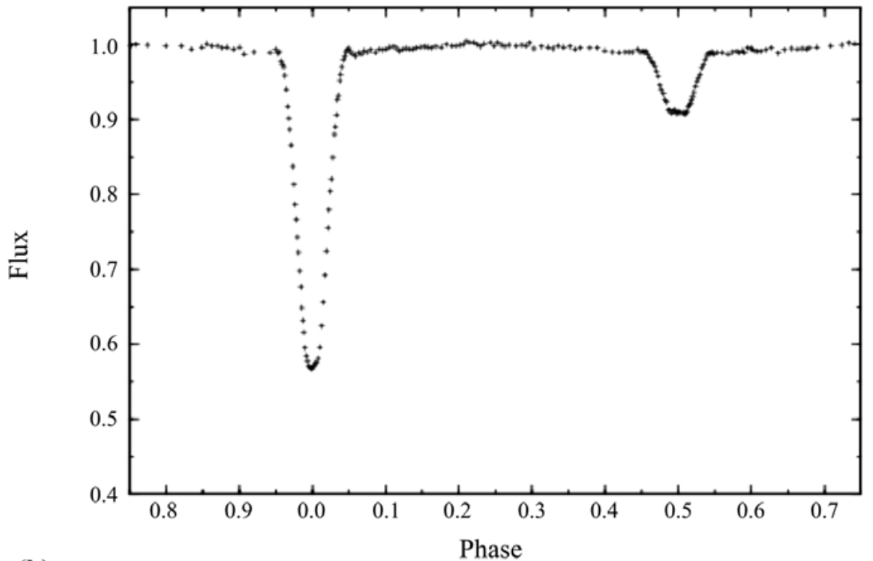
\includegraphics[scale=0.6]{Introduccion/Figures/Figura EA Curva_Modelling of WUMa Stars.png}
	\caption{Curva de luz emblemática de un sistema eclipsante
	\textit{EA}. Obtenida de
	\citeyearparen{skelton_modelling_wuma_variable_stars_2009}.}
	\label{figuraEACurvaLuz}
\end{figure}

\subsection{EB - \textbeta \ Lyrae}

En el caso de un sistema eclipsante semi-separado, la curva de luz observada se
le clasifica como tipo \textit{EB}, o de tipo \textbeta \space Lyrae. En un sistema
semi-separado una de las estrellas llena su lóbulo crítico de Roche, haciendo
contacto con la superficie de su compañera. Esta distorsión es responsable de su
forma elipsoidal en vez de esférica. El flujo que un observador recibe de una
estrella es proporcional al área superficial visible en la línea de visión; en
una estrella esférica, esta área es constante en el tiempo, pero en el caso de
una estrella elipsoidal la cantidad de área observada depende de la fase orbital
actual. Esto resulta en eclipses sin un comienzo y fin claramente delimitados.
En la mayoría de los casos el periodo orbital de este tipo de sistemas es mayor
de 1 día \citeyearparen{samus_gcvs_variable_types_2016}. 

\begin{figure}[!ht]
	\centering
	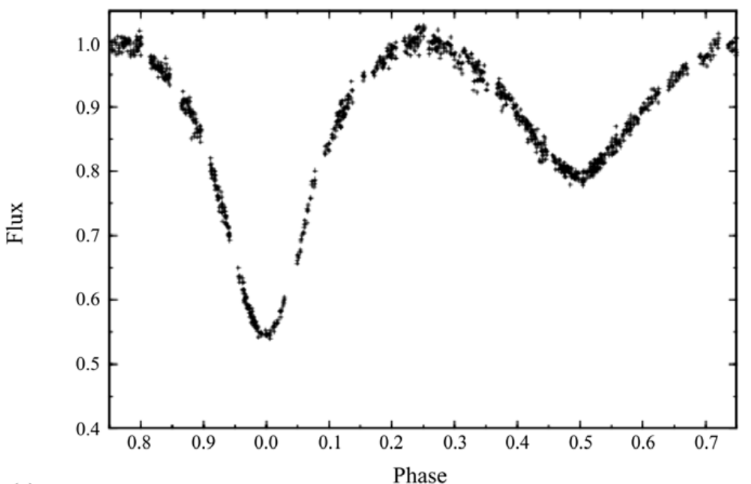
\includegraphics[scale=0.63]{Introduccion/Figures/Figura EB Curva_Modelling of WUMa Stars.png}
	\caption{Curva de luz emblemática de un sistema eclipsante
	\textit{EB}. Obtenida de
	\citeyearparen{skelton_modelling_wuma_variable_stars_2009}.}
	\label{figuraEBCurvaLuz}
\end{figure}

\subsection{EW - W UMa}

Sistemas en sobre-contacto, en donde ambas componentes llenan su lóbulo de
Roche, producen curvas de luz que muestran variabilidad continua a lo largo de
su órbita, parecido a los sistemas \textit{EB}. Sin embargo, a diferencia de los
sistemas semi-separados, ambas componentes de sistemas tipo \textit{EW} están
altamente acopladas una a otra, la diferencia de temperaturas siendo del orden
de cientos de Kelvin\textemdash lo cual es evidente por la profundidad de ambos
eclipses\textemdash de tipo espectral A-K
\citeyearparen{skelton_modelling_wuma_variable_stars_2009}. El periodo orbital es
menor de 1 día, del orden de unas cuantas horas, debido a su corta aproximación
física. La envoltura común que comparten las estrellas es de una forma
irregular; esta consiste de las superficies elipsoidales de las estrellas y del
\quotes{cuello}, la región que llena el espacio alrededor del punto de Lagrange
L1. Debido a esta geometría, cada fase orbital muestra una cantidad distinta de
la superficie del sistema, causando la variabilidad continua en la curva de luz,
sin una clara delimitación para ninguno de los eclipses. La
\reffigure{figuraEWCurvaLuz} muestra una curva de luz típica de un sistema
\textit{EW}. 

Una característica única de los sistemas \textit{EW} es la diferencia en los
máximos de la curva de luz. En ciertos casos puede ocurrir que un máximo del
flujo sea mayor que el máximo medido de el eclipse contrario, a pesar de estar
viendo una cantidad similar de superficie estelar. Este fenómeno observacional
es denominado el \textit{efecto O'Connell}. A pesar de que aún no es muy bien
entendido la causa de este efecto, una de las interpretaciones más populares en
la literatura es la presencia de manchas estelares
[\citeyearparen{ding_fast_derivation_cbs_params_2022}
\citeyearparen{michel_photometric_study_contact_binary_2023}
\citeyearparen{michel_rotse1_new_wuma_eclipsing_binary_2016}], las cuales al ser más
frías que el resto de la superficie llega a manifestar como una menor cantidad
de radiación emitida por el sistema en ciertas fases. Esto se atribuye a la
actividad magnética de la estrella, y se utiliza principalmente al momento de
ajustar un modelo computacional a la curva de luz observada.

\begin{figure}[!ht]
	\centering
	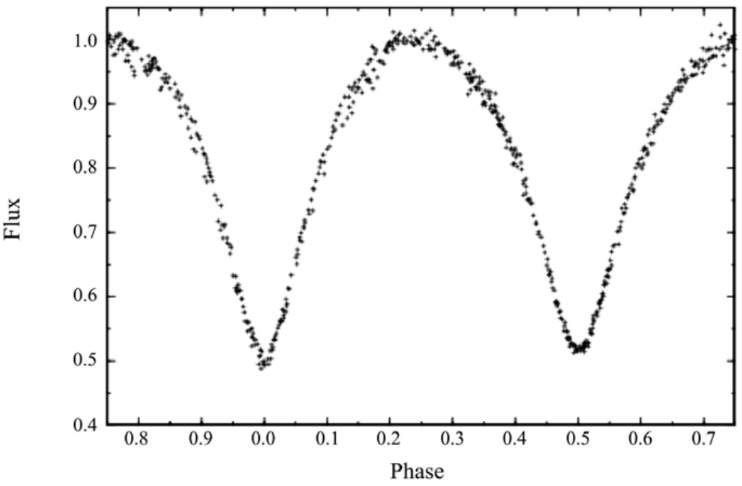
\includegraphics[scale=0.63]{Introduccion/Figures/Figura EW Curva_Modelling of WUMa Stars.png}
	\caption{Curva de luz emblemática de un sistema eclipsante
	\textit{EW}. Obtenida de
	\citeyearparen{skelton_modelling_wuma_variable_stars_2009}.}
	\label{figuraEWCurvaLuz}
\end{figure}
\chapter{PHOEBE - Modelo Computacional}

Utilizando el modelo de Roche combinado con el modelo de transporte de radiación
en el interior estelar, es posible generar una curva de luz observable sintética
de un sistema binario estelar, dado los parámetros físicos del sistema. Para
realizar esta tarea se utilizan códigos computacionales que integran las
ecuaciones planteadas en el \refthesischapter{capituloSistemasBinarios}. El uso
principal de estos modelos sintéticos computados es en la comparación con curvas
reales observadas de sistemas binarios; los parámetros del modelo se pueden
ajustar de tal manera que se encuentre la mejor combinación de valores que
resulten en una curva sintética (fotométrica en el caso de una curva de luz,
velocidades radiales, etc.) cuya diferencia con la curva observada sea la menor
posible. El proceso del ajuste del modelo es laborioso, por lo cual se han
desarrollado códigos que proporcionan herramientas para facilitar esta tarea.

En el campo de sistemas binarios estelares, uno de los primeros códigos con
mayor impacto es el código \textbf{Wilson-Devinney}, descrito por primera vez en
\citeyearparen{wilson_devinney_realization_of_accurate_binary_lcs_wd_1971}. El
código de Wilson-Devinney\textemdash referenciado como el código \textbf{WD} en
varias publicaciones\textemdash parte del modelo de Roche para representar las
superficies de las estrellas, lo cual le permite hacer un trato adecuado de
fenómenos físicos importantes como el oscurecimiento al limbo y el
oscurecimiento gravitacional. A pesar de sobrepasar 5 décadas de edad el código
WD sigue en uso actualmente en proyectos de investigación (por ejemplo,
\citeyearparen{li_extremely_low_mass_ratio_wd_analysis_2022}), de los cuales se
obtienen los parámetros físicos de un sistema binario estelar observado. Este
trabajo de tesis de maestría utilizó la librería \textbf{PHOEBE}
(\textbf{PH}ysics \textbf{O}f \textbf{E}clipsing
\textbf{B}inari\textbf{E}s\footnote{\url{http://phoebe-project.org}}), basado en
el código WD. En particular se hizo uso de la versión 2.4.13, notando las varias
mejoras realizadas en esta segunda versión mayor en comparación con versiones
menores a 2.0, las cuales utilizaban el código WD como el motor principal del
modelo.

\section{Estructura de PHOEBE} \label{intro:phoebe:estructura_phoebe}

PHOEBE es un paquete de software escrito en Python para generar modelos de
sistemas binarios estelares generales, partiendo del modelo de Roche y modelos
de atmósferas estelares, produciendo datos sintéticos (curvas de luz
fotométricas, velocidades radiales, perfil de líneas espectrales, etc.) para
analizar y comparar con datos observados reales. Es posible crear un modelo
utilizando un cliente
gráfico\footnote{\protect\url{http://phoebe-project.org/clients}} de PHOEBE,
cuya funcionalidad depende de un servidor de PHOEBE (una instancia de
\code{phoebe-server}) corriendo, de manera remota o local. Sin embargo, estas
tienen sus limitaciones, y por lo general el equipo de PHOEBE recomiendan usar
el paquete de Python de manera directa, escribiendo códigos en Python que llamen
a funciones y manipulen los parámetros del modelo. Un código escrito y ejecutado no
solo ofrece un mayor grado de libertad al momento de tratar los datos, si no que
sirve como una receta que cualquiera puede analizar y ejecutar para obtener los
mismos resultados de un experimento. Este trabajo de tesis unicamente hizo uso
del paquete de PHOEBE en Python.

PHOEBE maneja cada sistema modelado como un \textit{bundle}, el objeto principal
responsable de almacenar no solo los parámetros del sistema, pero también los
datos observados que corresponden al sistema físico. La
\refcode{codigoCreandoPhoebeBundle} presenta un ejemplo de como crear un
bundle de PHOEBE utilizando una curva de luz sintética (que solo se va a
utilizar al momento de computar la curva observable del modelo, sin una
contraparte real) y datos reales obtenidos del catálogo ZTF:

\begin{figure}[!ht]
	\begin{lstlisting}[language=Python, autogobble]
	import pandas as pd # paquete de manipulacion de datos
	import phoebe # importar el paquete

	# creando el bundle para un sistema binario en contacto
	b = phoebe.default_contact_binary() 

	# agregando una curva de luz en el pasabanda Johnson:V para computar (no datos reales)
	b.add_dataset('lc', times=phoebe.linspace(0, 1, 101), dataset='lc01', passband='Johnson:V')

	# datos obtenidos del catalogo de ZTF; curva de luz fotometrica, en el pasabanda ZTF:g
	ztf_data: pd.Dataframe

	# agregando curva de luz observada por ZTF, incluyendo el flujo medido y su incertidumbre
	b.add_dataset('lc', times=ztf_data['times'], fluxes=ztf_data['fluxes'], sigmas=ztf_data['flux_err'], passband='ZTF:g', dataset='lcZtfG')
	\end{lstlisting}
	\caption{Código para crear un bundle en PHOEBE junto a dos curvas de luz:
	\code{lc01}, una curva sintética en el pasabanda \textit{Johnson:V}, y
	\code{lcZtfG}, una curva observada del sistema con datos proveniente de el
	catálogo de ZTF en el pasabanda \textit{ZTF:G}. En el caso de \code{lc01},
	solo se generarán datos sintéticos al momento de calcular el \textbf{modelo
	hacia adelante}.}
	\label{codigoCreandoPhoebeBundle}
\end{figure}

A diferencia de otros códigos en el mundo de software, PHOEBE no utiliza mucho
la programación orientada a objetos para manipular el modelo (por ejemplo
manipulando un objeto que represente la estrella primaria); la arquitectura de
PHOEBE consolida todos los parámetros al nivel del bundle, tanto para tener
acceso conveniente para tener flexibilidad en cambiar el modelo de manera
dinámica\textemdash por ejemplo agregando una componente de luz externa al
sistema. Los parámetros de un bundle están organizados en una jerarquía, en
donde un identificador no es único en un solo nivel. Por ejemplo, el código para
inspeccionar la temperatura efectiva de la estrella primaria y asignar un valor
a la temperatura efectiva de la estrella secundaria se puede ver en la
\refcode{codigoAsignandoTeffPhoebe}.

\begin{figure}[!ht]
	\begin{lstlisting}[language=Python, autogobble]
	b: phoebe.Bundle # bundle de un sistema binario creado en un codigo anterior
	teff_primary = b.get_value(qualifier='teff', component='primary')
	b.set_value(qualifier='teff', component='secondary', value=teff_primary/2)
	\end{lstlisting}
	\caption{Definiendo un bundle almacenado en la variable \code{b}, el cual ya
	está configurado con ciertos parámetros del sistema. Estos son accesibles
	dentro del bundle; esto facilita la manipulación de parámetros del sistema
	programática, como se puede ver en este ejemplo al asignar el valor de la
	temperatura efectiva de la estrella secundaria como la mitad de la
	temperatura efectiva de la componente primaria.}
	\label{codigoAsignandoTeffPhoebe}
\end{figure}

Los parámetros de un bundle están organizados de tal manera que existen más de
un parámetro con el calificador (\code{qualifier} por su nombre en inglés y su
nombre en el código) \code{teff}. Estos se diferencian por la componente
(\code{component} en el código) a la que le pertenecen, en donde \code{primary}
se refiere a la estrella primaria y \code{secondary} a la secundaria, por sus
identificadores respectivos en inglés. Más información\textemdash incluyendo la
información más actual en el caso de ver una versión de PHOEBE diferente a
2.4.13\textemdash se puede encontrar en la página de documentación de
PHOEBE\footnote{\url{http://phoebe-project.org/docs/2.4/tutorials/general_concepts}}.

\section{\quotes{Modelo Hacia Adelante}}

El propósito principal de librerías como PHOEBE cae en su capacidad para generar
un \quotes{\textbf{modelo hacia adelante}} (traducido de forma directa de su nombre
en inglés: \textbf{forward model}). Parte de un modelo del sistema\textemdash
en el caso de un sistema binario, este viene siendo el modelo de Roche junto a
una formulación de las superficies estelares\textemdash el cual se va integrando
en el tiempo, produciendo como resultado datos sintéticos observables como una
curva de luz fotométrica o una curva de velocidades radiales. Un ejemplo de un
sistema \quotes{de juguete} se puede ver en la
\reffigure{figuraPhoebeObservablesSinteticos}. Es importante notar que estos
modelos se trabajan en el espacio fase de la órbita de un sistema; en casos
donde el sistema no experimente algún cambio significativo a lo largo del
tiempo, es suficiente computar el modelo para cada fase orbital observada, dado
que una campaña de observación adecuada abarcaría las mismas fases orbitales más
de una vez.

\begin{figure}[!ht]
	\centering
	\xincludegraphics[scale=0.253, label=\textbf{a)}, labelbox=true, pos=nw, fontsize=\Large]{Introduccion/Figures/Figura PHOEBE LC Sintetico.png}
	\xincludegraphics[scale=0.253, label=\textbf{b)}, labelbox=true, pos=nw, fontsize=\Large]{Introduccion/Figures/Figura PHOEBE RVs Sintetico.png}
	\caption{Datos sintéticos generados usando PHOEBE. Estas curvas representan
	un sistema binario separado, donde $M_1 = 1.0 \ \mathrm{M}_{\odot}$, $M_2 =
	0.5 \ \mathrm{M}_{\odot}$, $R_1 = 2.0 \ \mathrm{R}_{\odot}$, $R_2 = 1.2 \
	\mathrm{R}_{\odot}$, $T_1 = T_2 = 6000 \ \mathrm{K}$, inclinación
	$i_{\mathrm{orb}} = 90^{\circ}$ y periodo orbital $P_{orb} = 1.0 \
	\mathrm{d}$ en una órbita sincrónica. La figura muestra dos diferentes tipos
	de observables: \textbf{a)} Curva de luz fotométrica, cuyas variaciones se
	deben a los eclipses en el sistema. \textbf{b)} Curva de velocidades
	radiales de ambas componentes, donde el movimiento de las estrellas
	individuales a lo largo de nuestra línea de visión causa fluctuaciones
	debido al efecto de Doppler.} 
	\label{figuraPhoebeObservablesSinteticos}
\end{figure}

Para generar datos sintéticos observables de un sistema binario, es necesario
que PHOEBE tome ciertos aspectos en consideración, descritos a continuación en
este capitulo.

\subsection{Discretización de la Superficie Estelar}

Partiendo del modelo de Roche se determinan las superficies de ambas
componentes, siguiendo el principio de superficies equipotenciales. Sin embargo,
una descripción analítica de las variaciones de las propiedades estelares
resultaría en una complejidad de tiempo intratable del problema; a pesar de
permitirnos modelar pequeñas variaciones en los valores de cada parámetro
superficial, este no es una opción realista dado la capacidad de computo actual.
Es por esto que PHOEBE implementa un método el cual aproxima la superficie de
las estrellas a un muestreo uniforme de puntos determinados por el modelo de
Roche. Sin embargo, se requiere un tratamiento adicional del modelo de Roche; la
\refequation{ecuacionRocheExcentricaAsincronica} viene definida en coordenadas
esféricas, lo cual causaría una distribución no uniforme en el tamaño de los
elementos superficiales no deseada (aparte de causar un tipo de \quotes{costura}
a lo largo del ecuador de la estrella \citetbooksection{phoebeScientificReference}{5.1.1}).

Para resolver este problema, se transforma la
\refequation{ecuacionRocheExcentricaAsincronica} a un sistema de coordenadas
cilíndrico de acuerdo a las siguientes transformaciones:

\begin{eqfloat}[!ht]
	\centering
	\begin{equation}
		\begin{split}
			& x = \varrho_{\perp} \cos{\phi} \\
			& y = \varrho_{\perp} \sin{\phi} \\
			& z = z
		\end{split}
	\end{equation}
\end{eqfloat}

Donde $\phi$ representa la longitud, $\varrho_{\perp}$ es la componente en el
plano orbital de la distancia al elemento superficial, y $z$ mantiene su
definición del sistema de coordenadas cartesianas. Utilizando estas
transformaciones se llega a una expresión del potencial de Roche en coordenadas
cilíndricas:

% TODO: new page to group equation and text together
% \newpage

\begin{eqfloat}[!ht]
	\centering
	\begin{equation}
		\Omega = \frac{1}{\sqrt{\varrho_{\perp} + z^2}} + q \left(\frac{1}{\sqrt{\delta^2 + \varrho_{\perp}^2 + z^2 - 2 \varrho_{\perp} \delta \cos{\phi}}} - \frac{\varrho_{\perp} \cos{\phi}}{\delta^2} \right) + \frac{F^2 \left(1 + q\right) \varrho_{\perp}^2}{2}
	\end{equation}
	\blankcaption
	\label{ecuacionRocheCilindrica}
\end{eqfloat}

Parecido a la \refequation{ecuacionRadioPolarEstelarEquivalencia} se puede
llegar a una expresión similar para encontrar el valor de $\varrho_{\perp}$ que
le corresponde a los valores dados de $\phi$ y $z$, utilizando un método para
encontrar raíces como el de \textit{Newton-Raphson}:

\begin{eqfloat}[!ht]
	\centering
	\begin{equation}
		\begin{split}
			f(\varrho_{\perp}) = \eqnmark[MyDarkRed]{omega}{\frac{1}{\sqrt{\varrho_{\perp} + z^2}} + q \left(\frac{1}{\sqrt{\delta^2 + \varrho_{\perp}^2 + z^2 - 2 \varrho_{\perp} \delta \cos{\phi}}} - \frac{\varrho_{\perp} \cos{\phi}}{\delta^2} \right) + \frac{F^2 \left(1 + q\right) \varrho_{\perp}^2}{2}} \\
			\eqnmark[MyDarkBlue]{omegaPol}{- \frac{1}{z_{\textrm{pol}}} - \frac{q}{\sqrt{z_{\textrm{pol}}^2 + \delta^2}}}
		\end{split}
	\end{equation}
	\annotate[yshift=-0.3em]{below, left}{omega}{Potencial de Roche $\Omega$}
	\annotate[yshift=-0.2em]{below, left}{omegaPol}{Potencial de referencia en el polo $\Omega_{\mathrm{pol}}$}
	\blankcaption
	\vspace{0.4em}
	\label{ecuacionRadioCilindrica}
\end{eqfloat}

Donde se define $z_{\mathrm{pol}} \equiv \varrho_{\mathrm{pol}}$ como el valor
de referencia del radio al polo de la estrella
\citetbooksection{phoebeScientificReference}{5.1.1}. Al hacer uso de la derivada
$f' (\varrho_{\perp})$\textemdash la cual se puede obtener como lo muestra
\citetbooksection{phoebeScientificReference}{5.1.1}\textemdash es posible
implementar un método para encontrar las raíces de esta ecuación. El muestreo de la superficie se hace a intervalos regulares de latitud y longitud:

\begin{eqfloat}[!ht]
	\centering
	\vspace{0.6em}
	\begin{equation}
		\begin{split}
			& \eqnmark[MyDarkGreen]{lat}{\theta_k} = \frac{\pi \left(k - 0.5\right)}{2 N} \\
			& \eqnmark[MyLightBlue]{lon}{\phi_l} = \frac{\pi \left(l + \left[(l + 1) \textrm{mod} \ 2\right] \div 2 \right)}{M_k}
		\end{split}
	\end{equation}
	\annotate[yshift=1.1em]{above, left}{lat}{Latitud}
	\annotate[yshift=-0.2em]{below, left}{lon}{Longitud}
	\vspace{0.4em}
\end{eqfloat}

Donde $N$ es el número de elementos superficiales solicitados en la muestra. Se
define los subindices $k = 1 \dots N$ y $l = 1 \dots M_k$, donde $M_k := 1 +
\mathrm{int}\left(1.3 N \sin{\theta_k}\right)$
\citetbooksection{phoebeScientificReference}{5.1}. Una vez que se obtienen las
posiciones de cada muestra se adopta una forma tal que forme una \quotes{malla}
que representa la superficie estelar. Cada elemento de la malla se considera
uniforme con respecto a sus propiedades, como su temperatura efectiva, gravedad
superficial, el radio local, etc. En PHOEBE v2.0 y en adelante se utilizan
elementos en forma de triángulos equiláteros, tal como se muestra en la
\reffigure{figuraMallaPhoebe}. 

\begin{figure}[!ht]
	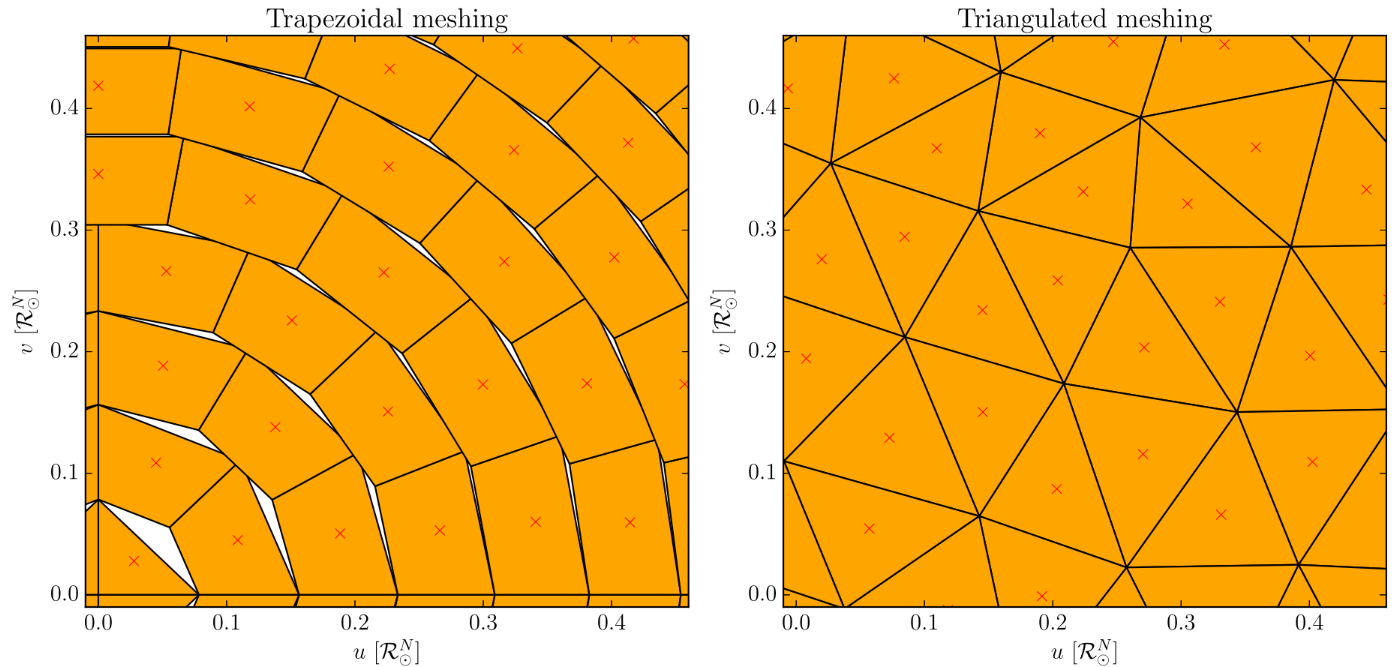
\includegraphics[scale=0.45]{Introduccion/Figures/Figura Mallado Triangular_PHOEBE II Mesh.png}
	\caption{Comparación la discretización superficial usando elementos
	trapezoidales vs. triangulares en el polo estelar. Al utilizar elementos de
	área superficial idéntica se nota que en el caso de elementos trapezoidales
	llega a haber huecos en la superficie que se manifiestan en errores
	sistemáticos en las curvas sintéticas generadas por el modelo, debido a la
	contribución nula de estas fallas en la malla. Estos errores se ven más
	pronunciados entre mayor sea la distorsión experimentada por la estrella. Al
	utilizar elementos en forma de triángulos equiláteros se puede observar que
	se obtiene una superficie continua, eliminando esta fuente de error en el
	modelo. Figura obtenida de
	\citeyearparen{prsa_phoebe_increased_model_fidelity_mesh_2016}}
	\label{figuraMallaPhoebe}
\end{figure}

Esta malla de la superficie estelar se puede ver por completo en la
\reffigure{figuraPhoebeMalla}, donde los parámetros del sistema causan una
distorsión apreciable de ambas estrellas debido a las fuerzas de marea en juego.

\begin{figure}[!ht]
	\centering
	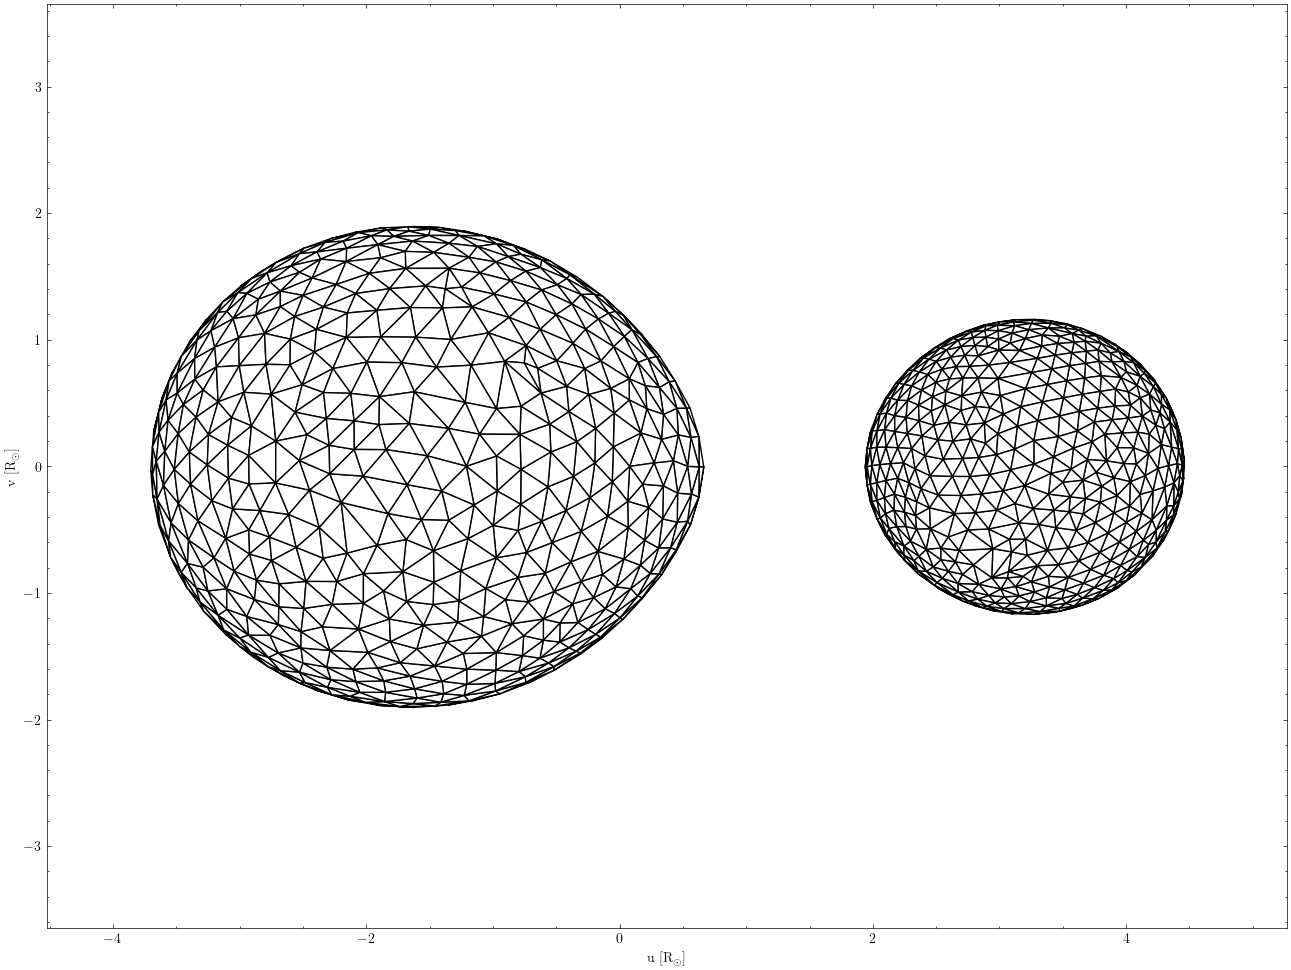
\includegraphics[scale=0.42]{Introduccion/Figures/Figura PHOEBE Malla.png}
	\caption{Mallas de las superficies estelares de un sistema simulado con
	PHOEBE, utilizando los mismos parámetros del modelo utilizado en la
	\reffigure{figuraPhoebeObservablesSinteticos}.}
	\label{figuraPhoebeMalla}
\end{figure}

La malla, al igual que la superficie estelar, no es un objeto constante; en el
caso de un sistema binario de órbita excéntrica las fuerzas de marea que causan
estas distorsiones elipsoidales son dependientes de la fase orbital. A lo largo
de la órbita del sistema, el campo del potencial de Roche va cambiando debido a
la distancia no constante entre ambas componentes estelares. Uno de los
principios del modelo de Roche es que las superficies estelares se ajustan al
campo de fuerzas instantáneo del sistema, el cual va cambiando a escalas de
tiempo significativamente menores que el periodo orbital
\citeyearparen{prsa_phoebe_increased_model_fidelity_mesh_2016}. Esto causaría un
cambio apreciable en los radios estelares, debido a que las superficies
equipotenciales del campo no son constantes en volumen. En teoría, si una
estrella se rige a solo las superficies equipotenciales del mismo valor en cada
fase orbital, la estrella debería de comprimirse o expandirse, irradiando parte
de su energía a su ambiente exterior, llegando rápidamente a una órbita
circular. Sin embargo, en la literatura no existen observaciones publicadas que
apoyen esta teoría; al contrario, existen sistemas como las estrellas
\quotes{heartbeat} (nombrado por su parecido a una lectura de un
electrocardiograma) cuya variabilidad se debe a la distorsión de sus superficies
por fuerzas de marea en órbitas excéntricas
\citeyearparen{thompson_class_eccentric_binaries_tidal_distortion_heartbeat_2012}.
Como consecuencia, PHOEBE adopta un mecanismo para preservar el volumen del
sistema; al momento de muestrear la superficie para generar la malla
superficial, PHOEBE elige la superficie equipotencial que más se acerque al
volumen calculado de las estrellas en su punto de periastro, el punto en donde
experimentan la mayor distorsión superficial.

\subsection{Distribución de Parámetros Superficiales}

Una estrella no es perfectamente uniforme en la superficie; un modelo acertado
de una estrella debe tomar en cuenta la distribución de parámetros como su
temperatura, intensidad, etc. Para esto se debe calcular la gravedad superficial
en el polo estelar:

\begin{eqfloat}[!ht]
	\centering
	\begin{equation}
		\textbf{g}_{\textrm{pol}} = -\frac{G m_1}{r_{\textrm{pol}}^2} \frac{\textbf{r}_{\mathrm{pol}}}{r_{\mathrm{pol}}} - \frac{G m_2}{h^2} \frac{\textbf{h}}{h} - \omega^2(t) d_{\perp,\textrm{rot}} \frac{\textbf{d}_{\perp,\textrm{rot}}}{d_{\perp,\textrm{rot}}} 
	\end{equation}
\end{eqfloat}

Donde se define $r_{\mathrm{pol}}$ como el radio al polo estelar, $h =
\sqrt{r_{\mathrm{pol}}^2 + d^2}$ es la distancia del polo estelar al centro de
la estrella compañera, $\omega(t)$ es la velocidad angular como función del
tiempo, y $d_{\perp,\textrm{rot}}$ es la distancia del polo estelar hacia el eje
de rotación del sistema (su centro de masa)
\citetbooksection{phoebeScientificReference}{5.2}. La gravedad superficial
depende de manera indirecta de la fase orbital, debido al ajuste de la estrella
a una superficie equipotencial a lo largo de la órbita del sistema. Este
parámetro rige la distribución de material y energía en la estrella; las
regiones de mayor gravedad superficial (en sistemas binarios eclipsantes suelen
ser los polos estelares, debido a las fuerzas de marea que resultan en un radio
ecuatorial mayor) con áreas más calientes que el resto de la superficie.
\citetbooksection{phoebeScientificReference}{4.3} dice que el flujo
monocromático para el rango de longitud de onda $[\lambda, \lambda +
\mathrm{d}\lambda]$ es proporcional tanto a la gravedad superficial como a la
temperatura efectiva:

\begin{eqfloat}[!ht]
	\centering
	\begin{equation}
		F_{\lambda} = - \frac{16 \sigma T_{\textrm{eff}}^3}{3 \bar{\kappa} \rho} \frac{\textrm{d}T_{\textrm{eff}}}{\textrm{d}\Omega} g^{\beta}
	\end{equation}
\end{eqfloat}

Donde $\sigma = 5.67 \times 10^{-8} \mathrm{W} \mathrm{m}^{-2} \mathrm{K}^{-4}$
es la constante de Stefan-Boltzmann, $\bar{\kappa}$ es el coeficiente de
opacidad de Rosseland (el cual describe la opacidad, o la probabilidad de un
fotón de atravesar un medio\textemdash en este caso la superficie estelar),
$\rho$ es la densidad del material en la fotósfera, $g$ es la aceleración
gravitacional local, y $\beta$ es el \textit{coeficiente del oscurecimiento
gravitacional}. El valor de $\beta$ en lo general se mantiene fijo dependiendo
de la naturaleza de la envoltura estelar:

\begin{eqfloat}[!ht]
	\centering
	\begin{equation}
		\beta = \left\{\begin{matrix}
			0.32 & \textrm{envoltura convectiva} & T_{\textrm{eff}} < 5000 \ \textrm{K} \\
			1 & \textrm{envoltura radiativa} & T_{\textrm{eff}} > 8000 \ \textrm{K} \\
			\end{matrix}\right. 
	\end{equation}
\end{eqfloat}

Utilizando este coeficiente es posible calcular la temperatura y el flujo de un
elemento superficial dependiendo de la aceleración gravitacional local, dado un
valor de referencia que corresponde al polo estelar:

\begin{eqfloat}[!ht]
	\centering
	\begin{equation}
		\begin{split}
			& F = F_{\textrm{pol}} \left(\frac{g}{g_{\textrm{pol}}}\right)^{\beta} \\
			& T_{\textrm{eff}} = T_{\textrm{eff},\textrm{pol}} \left(\frac{g}{g_{\textrm{pol}}}\right)^{\beta/4}
		\end{split}
	\end{equation}	
\end{eqfloat}

De la cual se obtiene el flujo y la temperatura efectiva dada una aceleración
gravitacional local, donde el término
$\left(g/g_{\mathrm{pol}}\right)^{\beta/4}$ se conoce como la \textbf{corrección
del oscurecimiento gravitacional}. La superficie resuelta con respecto a su
gravedad superficial y temperatura efectiva se puede ver en la
\reffigure{figuraMallaPhoebeTeffLogg}.

\begin{figure}[!ht]
	\centering
	\xincludegraphics[scale=0.27, label=\textbf{(a)}, labelbox=true, pos=nw, fontsize=\Large]{Introduccion/Figures/Figura PHOEBE Malla Logg.png}
	\xincludegraphics[scale=0.27, label=\textbf{(b)}, labelbox=true, pos=nw, fontsize=\Large]{Introduccion/Figures/Figura PHOEBE Malla Teff.png}

	\caption[Distribución de gravedad superficial y temperatura efectiva
	local.]{Malla de una estrella cuyas propiedades son las mismas que el Sol,
	generada utilizando PHOEBE, donde el potencial efectivo es calculado no en
	base al modelo de Roche, si no basado en su frecuencia de rotación, en el
	caso de una estrella aislada\textemdash a pesar de que esta información no
	esté documentada explícitamente en un documento fácil de encontrar, esto se
	puede ver en el código fuente de PHOEBE 2, en este caso en el archivo
	\href{https://github.com/phoebe-project/phoebe2/blob/master/phoebe/distortions/rotstar.py}{\code{rotstar.py}}.
	Se puede ver la distribución de gravedad efectiva superficial en el índice
	\textbf{(a)}, al cual se acopla la distribución de temperatura efectiva
	vista en el índice \textbf{(b)}.}
	\label{figuraMallaPhoebeTeffLogg}
\end{figure}

% TODO: formatting new page
\newpage

\subsection{Radiación Emergente}

Una vez determinada la distribución de parámetros superficiales es posible
determinar la radiación emergente de cada elemento superficial, del cual se
calcula el flujo que recibe un observador. El flujo de una estrella no es una
cantidad que PHOEBE determina directamente; PHOEBE más bien calcula la
\textit{intensidad}, que se define como la cantidad de energía $\mathrm{d}E$
emitida a través de el ángulo solido $\mathrm{d}\Omega$ por una superficie
proyectada a un ángulo $\mathrm{d}A \cos{\theta}$ en el intervalo de tiempo
$\mathrm{d}t$:

\begin{eqfloat}[!ht]
	\centering
	\begin{equation}
		I_{\lambda} = \frac{\textrm{d}E}{\textrm{d}\lambda \textrm{d}A \cos{\theta} \textrm{d}\Omega \textrm{d}t}
	\end{equation}
	\blankcaption
	\label{ecuacionIntensidadMonocromatica}
\end{eqfloat}

Donde $I_{\lambda}$ es la \textit{intensidad monocromática}, para un intervalo
de longitud de onda $[\lambda, \lambda + \textrm{d}\lambda]$. Esta cantidad es
calculada en la dirección normal de cada elemento superficial; la
\reffigure{figuraMallaPhoebeIntensidadNormal} muestra la distribución de
intensidad absoluta a lo largo de la superficie estelar. La intensidad
monocromática se obtiene partiendo del modelo atmosférico empleado, ya sea el de
cuerpo negro básico o una tabla como la de \citeyearparen{kurucz_atlas_1970}. Para
obtener la \textit{intensidad absoluta} es necesario integrar la intensidad
monocromática sobre todas las longitudes de onda:

\begin{eqfloat}[!ht]
	\centering
	\begin{equation}
		I = \int_{0}^{\infty}{I_{\lambda} \textrm{d}\lambda}
	\end{equation}
	\blankcaption
	\label{ecuacionIntensidadTotal}
\end{eqfloat}

\begin{figure}[!ht]
	\centering
	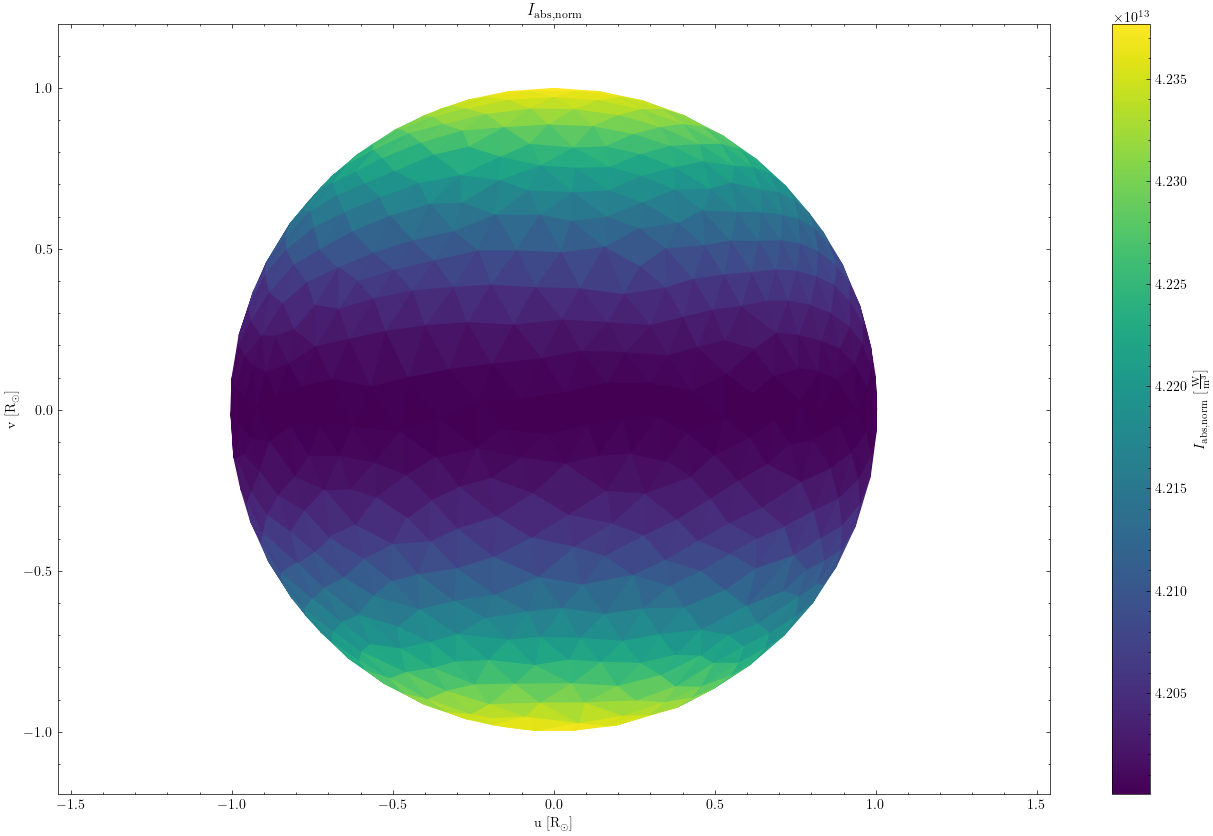
\includegraphics[scale=0.4]{Introduccion/Figures/Figura PHOEBE Malla Intensidad Normal.png}
	\caption{Intensidad absoluta de una estrella modelada utilizando PHOEBE,
	integrada en las longitudes de onda que abarca el pasa banda de
	\textit{Johnson:V}. La figura muestra la intensidad absoluta en la dirección
	del vector normal a los elementos superficiales. Se puede apreciar la
	distribución de la intensidad, la cual sigue el mismo comportamiento de la
	gravedad superficial que se muestra en la
	\reffigure{figuraMallaPhoebeTeffLogg}.}
	\label{figuraMallaPhoebeIntensidadNormal}
\end{figure}

Utilizando la intensidad monocromática dada por la
\refequation{ecuacionIntensidadMonocromatica} se usa para definir la
\textbf{distribución espectral de energía} (\textbf{SED} por sus siglas en
inglés), donde $\mathcal{S} \equiv \mathrm{d}I_{\lambda}/\mathrm{d}\lambda$. La
SED calculado depende tanto en las propiedades de la estrella como en el modelo
empleado para su atmósfera estelar; en el caso de un cuerpo negro, su SED
depende solo de su temperatura efectiva, mientras que modelos como
\citeyearparen{kurucz_atlas_1970} requieren parámetros adicionales como la
metalicidad estelar y gravedad superficial. Sin embargo, en el modelo hacia
adelante de una estrella es de gran importancia determinar la intensidad en una
\textit{pasa banda}; esta es definida por una curva de transmisión, la cual
describe la cantidad de radiación incidente que traspasa el sistema óptico.
PHOEBE tiene varias pasa bandas disponibles, como por ejemplo la de
\textit{Johnson:V} vista en la \reffigure{figuraPhoebePasabandaJohnsonV}.
Utilizando la pasa banda elegida y la SED calculado se computa la intensidad de
la pasa banda con la siguiente ecuación:

\begin{eqfloat}
	\centering
	\begin{equation}
		I_{\textrm{pb}} = \int_{\lambda}{\mathcal{S}(\lambda) \mathcal{P}(\lambda)\textrm{d}\lambda}
	\end{equation}
	\blankcaption
	\label{ecuacionIntensidadPasabanda}
\end{eqfloat}

Donde $I_{\mathrm{pb}}$ como $\mathcal{S}$ son funciones que toman de parámetro
de entrada las propiedades termodinámicas de la estrella, incluyendo incluso
efectos extrínsecos al sistema como la extinción interestelar
\citeyearparen{prsa_phoebe_increased_model_fidelity_mesh_2016}. La intensidad
$I_{\mathrm{pb}}$ definida en la \refequation{ecuacionIntensidadPasabanda} solo
es apropiada para simular un detector calibrado por flujo de estrellas
estándares; para medir la intensidad con respecto al número de fotones
detectados es necesario dividir $I_{\mathrm{pb}}$ entre la energía del fotón
incidente, definida como $E_{\lambda} = hc/\lambda$, e integrar:

\begin{eqfloat}
	\centering
	\begin{equation}
		I_{\textrm{pb}, \textrm{fot}} = \int_{\lambda}{\left(\frac{\mathcal{S}(\lambda) \mathcal{P}(\lambda)}{E_{\lambda}}\textrm{d}\lambda \right)} = \frac{1}{hc} \int_{\lambda}{\lambda \mathcal{S}(\lambda) \mathcal{P}(\lambda) \textrm{d}\lambda}
	\end{equation}
\end{eqfloat}

Por último, se integra $I_{\mathrm{pb}, \mathrm{fot}}$ o $I_{\mathrm{pb}}$\textemdash
dependiendo si se desea el flujo por cuentas de fotones o en energía\textemdash
a lo largo de la superficie estelar visible para obtener el flujo emitido por la
estrella en la pasa banda deseada, llegando como resultado a una curva de luz
sintética como en la \reffigure{figuraPhoebeObservablesSinteticos}, la cual
forma la base del análisis fotométrico de un sistema binario estelar.

\begin{figure}[!ht]
	\centering
	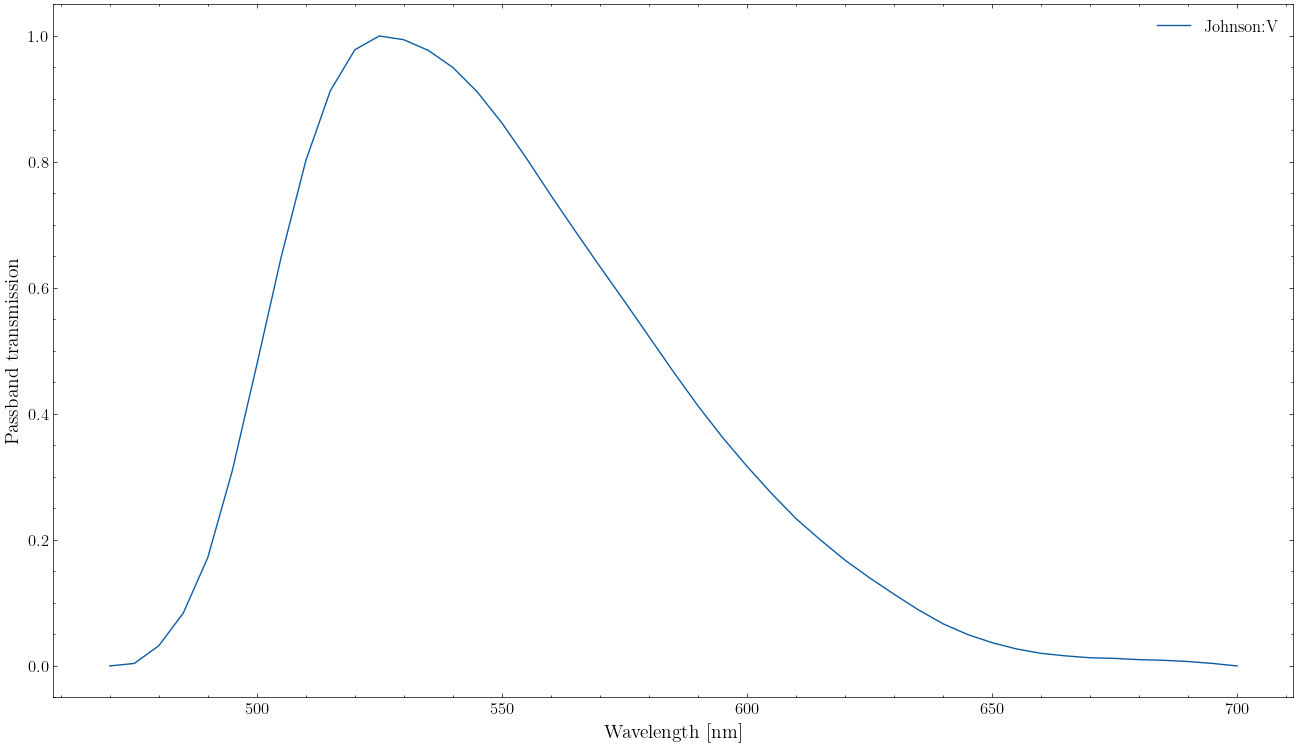
\includegraphics[scale=0.4]{Introduccion/Figures/Figura PHOEBE JohnsonV Pasabanda.png}
	\caption{Curva de transmisión en PHOEBE para la pasa banda \textit{Johnson:V}.}
	\label{figuraPhoebePasabandaJohnsonV}
\end{figure}

\section{El Problema Inverso}

El tener un modelo sofisticado de un sistema binario estelar nos ayuda a
entender los mecanismos responsables de su comportamiento, incluyendo como
afectan las diferentes combinaciones de parámetros estelares en las curvas
observables del sistema. Sin embargo, el propósito de modelos como PHOEBE o WD
yace en determinar los parámetros físicos que, una vez imputadas al modelo,
generan una curva observable sintética que se acopla a datos reales observados
del sistema. Esto en general se conoce como el \textbf{problema inverso}, y es
tanto una gran parte de este trabajo de tesis como el objetivo de varias
investigaciones en la literatura. Encontrar los parámetros que mejor ajustan un
modelo a datos observados es un proceso particular para cada objeto estudiado;
sin embargo, existe un proceso general que se sigue para llegar a una conclusión
cuyos errores y sesgos sean aceptables.

\subsection{Función de Calidad}

Para saber si un modelo es un buen ajuste a una curva observable de un sistema
es necesario definir una función que sirva para parametrizar el error entre el
modelo sintético y los datos reales. Para una curva observada, se calcula el
$\chi^2$, el cual se define como la siguiente expresión:

\begin{eqfloat}[!ht]
	\centering
	\begin{equation}
		\chi_{k}^2 = \sum_{i=1}^{N}{\left(\frac{y_{i,o} - y_{i,m}}{\sigma_{i}^2} + \ln{\sigma{i}^2}\right)}
	\end{equation}
	\blankcaption
	\label{ecuacionPhoebeChi2Curva}
\end{eqfloat}

Donde $y$ indica un punto en la curva del modelo, los subindices $o$ y $m$
refiriéndose a datos observacionales o del modelo sintético, respectivamente.
Cada punto del modelo se le atribuye un peso, la incertidumbre en el dato
observado $\sigma_{i,o}$, el cual se determina antes de ingresar los datos a
PHOEBE. En el caso de tener incertidumbres que han sido subestimadas se
introduce el termino $\sigma_{inf}$, donde al final se obtiene la incertidumbre
$\sigma_{i}$:

% TODO: formatting new page
\newpage

\begin{eqfloat}[!ht]
	\centering
	\begin{equation}
		\sigma_{i}^{2} = \sigma_{i,o}^{2} + y_{i,m}^{2} \exp{\left(2 \sigma_{inf}\right)}
	\end{equation}
\end{eqfloat}

En el caso de tener incertidumbres acertadas, $\sigma_{inf} = -\infty$, el cual
simplifica la previa ecuación a solo $\sigma_{i}^{2} = \sigma_{i,o}^{2}$.

Estos datos no necesariamente son mediciones fotométricas del sistema; pueden
ser velocidades radiales o intensidades de lineas espectrales. El subíndice $k$
denota la curva para la cual se está calculando el ajuste del modelo. Si se
tienen varias curvas observadas (por ejemplo, en diferentes bandas fotométricas)
el ajuste total del modelo se califica por la suma de los ajustes individuales a
cada curva observable:

\begin{eqfloat}[!ht]
	\centering
	\begin{equation}
		\chi^2 = \sum_{k}{\chi_{k}^{2}}
	\end{equation}
	\blankcaption
	\vspace{-0.4em}
	\label{ecuacionChi2}
\end{eqfloat}

El objetivo de un ajuste de un modelo a datos observacionales es encontrar los
parámetros físicos del sistema binario en cuestión que resultan en el $\chi^{2}$
más cercano a 0 posible. El valor obtenido de $\chi^2$ se parametriza en PHOEBE
normalizando por el número de observaciones hechas en todas las curvas de luz
combinadas $N_{\mathrm{tot}}$, resultando en el parámetro $\lambda$, el cual
indica un ajuste satisfactorio si $\lambda \approx 1$:

\begin{eqfloat}
	\centering
	\begin{equation}
		\lambda \coloneq \frac{\chi^2}{N_{\textrm{tot}}}
	\end{equation}
	\blankcaption
	\label{ecuacionLambdaCostoPhoebe}
\end{eqfloat}

Sin embargo, el modelo descrito en la literatura, y que
usa PHOEBE, es altamente no-lineal; el espacio de parámetros posee una topología
compleja, el cual implica que existen más de una combinación de valores para los
parámetros del modelo que se ajustan a un mismo conjunto de curvas
observacionales, el cual se resalta en casos de degeneración de un modelo, donde
2 o más parámetros se ven correlacionados de tal manera que existen una cantidad
infinita de soluciones al problema. 

Para finalizar la descripción de PHOEBE con
respecto a este trabajo de tesis, se describe un proceso de ajuste de modelo a
un conjunto de curvas de luz fotométricas, utilizando herramientas dadas dentro
de PHOEBE, con la finalidad de llegar a la mejor combinación de parámetros
evitando caer lo más posible en trampas como mínimos locales en el espacio de
parámetros y modelos degenerados.

\subsection{Estimación Inicial de Parámetros}

La solución final para un sistema binario va a depender de manera significativa
de los valores iniciales de los cuales parten las siguientes etapas del
ajuste. El proceso de estimar los valores iniciales es una combinación de
manipulación manual y herramientas diseñadas para un ajuste rápido a los datos
observacionales. Para utilizar estos estimadores es necesario primero encontrar
el periodo orbital del sistema, el cual comúnmente corresponde a la segunda
harmonica de la frecuencia dominante de un periodograma; los algoritmos
principales utilizados en la literatura son \textit{Lomb-Scargle}
\citeyearparen{vanderplas_understanding_lomb_scargle_periodogram_2018} el cual ajusta
un modelo sinusoidal a una serie de tiempo (cuyas muestras no requieren haber
sido tomadas en intervalos regulares del tiempo) y \textit{Box Least Squares}
(abreviado como BLS) \citeyearparen{kovacs_bls_periodogram_periodic_transits_2002},
un algoritmo diseñado para casos donde la señal de los eclipses es pequeña a
comparación con el flujo de base del sistema, por ejemplo los sistemas cuya
duración de eclipses estelares es mucho menor que el periodo orbital. Existen
varias implementaciones de periodogramas para su uso en el ámbito de la
astrofísica; ambos están disponibles dentro de PHOEBE en la forma de un
estimador:

\begin{figure}[!ht]
	\begin{lstlisting}[language=python, autogobble]
	periodogram_freqs = phoebe.linspace(0.001, MAX_FREQ, NUM_FREQS)
	b.add_solver('estimator.lc_periodogram', 
					solver='periodogram',
					algorithm='ls', # 'ls' corresponde a Lomb-Scargle, 'bls' a BLS
					sample_mode='manual',
					lc_datasets=['lc01', 'lc02'],
					sample_periods=periodogram_freqs)
	b.run_solver(solver='periodogram', solution='period_spectrum')
	\end{lstlisting}
	\caption{Ejemplo de cómo correr un periodograma de tipo
	Lomb-Scargle en un bundle de PHOEBE. Este caso en particular es para un
	modelo con 2 curvas de luz fotométricas distintas, que se ha determinado
	muestra un comportamiento sinusoidal. Dependiendo de la información
	antecedente disponible del objeto al estudiar se puede definir limites de
	manera manual del periodograma, por ejemplo si se sabe que es un sistema de
	corto periodo ($<$1 día). Los resultados del periodograma se pueden acceder en
	la solución \code{period\_spectrum}, donde se puede obtener el espectro de
	potencias completo.}
\end{figure}

Es posible correr un periodograma de manera automática o manual, dependiendo si
una malla de frecuencias es dada como entrada al periodograma. Una vez que se
obtenga el periodo orbital del sistema es posible determinar un punto de partida
de los parámetros del sistema, utilizando la curva de luz ajustada en fase.
Dentro de PHOEBE existen 2 distintos métodos para esto: la estimación de
parámetros utilizando de manera directa la geometría de la curva, o haciendo uso
de \textbf{EBAI}.

\subsubsection{Geometría de la Curva de Luz}
Dada una curva de luz fotométrica en fase es posible estimar ciertos parámetros
del sistema analizando ciertas características geométricas. Una vez que
se haya encontrado el periodo orbital del sistema\textemdash y por ende haber
obtenido la curva de luz en fase\textemdash es posible ajustar una función
analítica compuesta de 2 funciones Gaussianas, un término coseno, un término
constante, o cualquier combinación de estas que mejor se ajusten a los datos
observacionales, generando en total 7 modelos
\citeyearparen{conroy_phoebe_v_framework_solving_inverse_problem_2020}. Utilizando un
ajuste de mínimos cuadrados a las curvas en fase, una vez estimado los tiempos
de los eclipses, se determina el mejor modelo usando un criterio. Del modelo
final se obtienen valores iniciales tanto para propiedades orbitales del
sistema\textemdash el tiempo de superconjunción primario $t_0$, la excentricidad
$e$, y el argumento de periastro $\omega_0$\textemdash como propiedades
relativas entre las estrellas componentes: la suma de radios normalizado al
semieje mayor de la órbita $(R_1 + R_2)/a_{\mathrm{orb}}$ (esto se nota en la
diferencia de anchura entre ambas jorobas de la curva de luz) y la razón de
temperaturas efectivas $T_{\mathrm{eff},2}/T_{\mathrm{eff},1}$ (el cual se puede
aproximar por la diferencia de profundidad entre el eclipse primario y
secundario). Este estimador solo es capaz de analizar sistemas separados, por lo
cual no se utilizó en este trabajo de tesis.

\subsubsection{EBAI - Eclipsing Binaries via Artificial Intelligence} \label{intro:phoebe:problema_inverso:ebai}
\textbf{EBAI} es una red neuronal artificial que hace uso de métodos de
aprendizaje automático como \textit{K-Nearest Neighbors} para mapear una curva
de luz observacional a parámetros físicos de un sistema binario estelar. El
algoritmo KNN ajusta una función a datos reales, permitiendo hacer una regresión
basado en los vecinos cercanos de un punto. Los detalles de KNN se encuentran en
\citeyearparen{pedregosa_scikit-learn_2011}, el cual describe la implementación
dentro del paquete de Python \code{scikit-learn}. Una red neuronal es compuesta
de varias capas de procesamiento, donde cada capa está compuesta de unidades
individuales (o \quotes{neuronas}) que propagan valores de acuerdo a su función
de activación. Esta arquitectura es la que les permite \quotes{aprender}
relaciones en modelos no lineales como el de un sistema binario. Hasta el
momento (PHOEBE version $\leq$2.4.13) el estimador de EBAI es el único capaz de
estimar los parámetros de un sistema binario en contacto; un esquema de su
composición interna se puede ver en la \reffigure{figuraPhoebeEbaiAnnDiagrama}.

\begin{figure}[!ht]
	\centering
	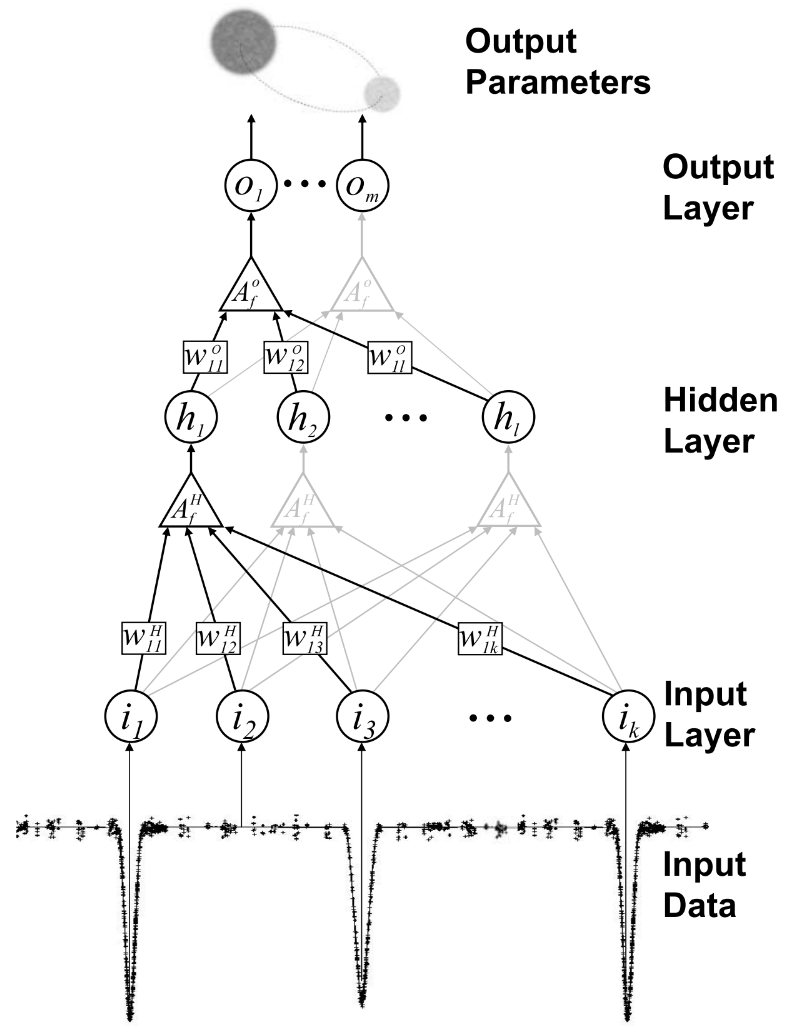
\includegraphics[scale=0.5]{Introduccion/Figures/Figura PHOEBE EBAI ANN Diagrama.png}
	\caption{Esquema de una red neuronal artificial (ANN por sus siglas en
	inglés). El objetivo de una red como EBAI es partir de datos de entrada como
	una curva de luz observada y obtener los parámetros del sistema que generen
	un modelo sintético que se aproxime a los datos. Figura obtenida de
	\citeyearparen{prsa_phoebe_artificial_intelligence_approach_ebai_2008}.}
	\label{figuraPhoebeEbaiAnnDiagrama}
\end{figure}

Para sistemas binarios en contacto, el estimador EBAI puede determinar la razón
de masa $q$, la razón de temperaturas efectiva $T_2/T_1$, la inclinación orbital
$i$, y el factor de relleno $f$ del sistema; el estimador calcula un valor para
el tiempo de superconjunción $t_0$ del sistema binario, el cual es necesario
para obtener una curva de luz en fase cuyo eclipse primario yace en la fase
orbital 0. Dado un Bundle en PHOEBE, se puede generar una estimación inicial
corriendo el siguiente código:

\begin{figure}[!ht]
	\begin{lstlisting}[language=Python, autogobble]
	# b: phoebe.Bundle
	b.add_solver('estimator.ebai', solver='ebai_estimator', 
					ebai_method='knn', phase_bin=False, 
					lc_datasets=['lc01', 'lc02'])
	b.run_solver(solver='ebai_estimator', solution='ebai_init_estimates')
	b.adopt_solution(solution='ebai_init_estimates')
	\end{lstlisting}
	\caption{Código para correr un estimador EBAI para un sistema compuesto de 2
	curvas de luz fotométricas distintas, \code{lc01} y \code{lc02}. Para un
	sistema binario separado también existe la opción de correr el estimador con
	\code{ebai\_method='mlp'}, el cual usa una red neuronal propia de PHOEBE.}
\end{figure}

\subsection{Optimización de Parámetros}

Durante un ajuste de modelo es importante determinar si la combinación de
parámetros elegida es óptima dado una serie de datos observados. Esto se basa en
la función de costo definida en la \refequation{ecuacionChi2}; un ajuste
adecuado del modelo implica tener un valor de $\chi^2$ cercano a 0. PHOEBE
ofrece herramientas especializadas para encontrar la combinación de parámetros
que más se acerca a esta condición de manera sistemática. Estos son denominados
\textit{optimizadores}: algoritmos diseñados para explorar el espacio de
parámetros y llegar a un mínimo de la función de costo. Este trabajo de tesis
hizo uso de 2 optimizadores principales: \textbf{el simplex de Nelder-Mead} y
\textbf{correcciones diferenciales}.

\subsubsection{Simplex de Nelder-Mead} \label{intro:phoebe:nelder_mead}

Descrito por primera vez por \citeyearparen{nelder_mead_simplex_1965}, el
\textbf{simplex de Nelder-Mead} (NMS por sus siglas en inglés) es un algoritmo
heurístico que explora el espacio de parámetros mediante un \textit{simplex}, un
politopo compuesto de varios vértices que representan distintos puntos en la
función que se busca optimizar. En el caso de PHOEBE, la función a optimizar es
$\chi^2$; para esto es necesario evaluar el ajuste en cada punto del simplex, lo
cual requiere calcular el modelo hacia adelante para cada punto de prueba. Esto
se demuestra con la siguiente modificación a la \refequation{ecuacionChi2}:

\begin{eqfloat}[!ht]
	\centering
	\begin{equation}
		\chi^2(\textbf{p}) = \sum_{i}{\frac{\left(F_{i}^{\textrm{obs}} - F^{\textrm{syn}}_i(\textbf{p})\right)^2}{\sigma_{i}^2}}
	\end{equation}
	\blankcaption
	\label{ecuacionChi2Params}
\end{eqfloat}

Donde $\mathbf{p}$ representa el vector de parámetros del modelo, como la
inclinación orbital, razón de masas, y cualquier otro incluido en el cálculo. El
método de NMS solo requiere evaluaciones de la función de costo en los puntos
del simplex; esto lo hace un método adecuado para optimizar funciones altamente
no-lineales a cambio de una baja eficiencia computacional 
dependiendo del número de vértices a evaluar. En total, la cantidad
de vértices empleados depende del número de dimensiones del modelo; en el caso
de optimizar $n$ parámetros del sistema binario, NMS utilizará $n+1$ vértices, o
combinaciones de parámetros. Con cada iteración, el método manipula el simplex
por medio de transformaciones geométricas, como lo muestra
\citetbooksection{phoebeScientificReference}{6.4}. En el ajuste de un sistema
binario eclipsante el método de NMS se utiliza para intentar llegar al mínimo
global de la función de costo, el cual el punto de parada es cuando haya
convergido la optimización (donde el simplex se podría considerar de un tamaño
geométrico despreciable), o cuando hayan pasado un cierto número de iteraciones,
en el caso que no haya sido completamente exitoso. Su uso se puede ver en la
\refcode{codigoOptimizadorNMS}. Para más información de la implementación y uso
del optimizador se puede hacer referencia a la documentación de
SciPy\footnote{\url{https://docs.scipy.org/doc/scipy/reference/optimize.minimize-neldermead.html}}.

\begin{figure}[!ht]
	\centering
	\begin{lstlisting}[language=Python, autogobble]
	# b: phoebe.Bundle
	b.add_solver('optimizer.nelder_mead', solver='opt_nm', maxiter=50,
		fit_parameters=['teffratio', 'period@binary', 
			't0_supconj@binary', 'incl@binary', 'fillout_factor'])
	b.run_solver(solver='opt_nm', solution='opt_nm_solution')
	\end{lstlisting}
	\caption{Código para crear y ejecutar un optimizador utilizando el algoritmo
	NMS. Este código en particular busca encontrar la combinación de la razón de
	temperaturas, periodo orbital, el tiempo de superconjunción primario, la
	inclinación orbital, y el factor de relleno del sistema, como se puede ver
	por el argumento \code{fit\_parameters} del resolvedor (\textit{solver} por
	su categoría en inglés). Se especifica 50 como el máximo número de
	iteraciones que tiene permitido correr el optimizador en dado caso que no
	llegue a converger a una solución; el criterio de convergencia se define por
	los argumentos \code{xatol} y \code{fatol} que definen una tolerancia de
	convergencia para los parámetros de entrada y la función de costo,
	respectivamente.}
	\label{codigoOptimizadorNMS}
\end{figure}

\subsubsection{Correcciones Diferenciales} \label{intro:phoebe:correcciones_diferenciales}

Una de las formas más directas de explorar el espacio de parámetros y llegar a
un valor óptimo de la función de costo es por el método de \textbf{correcciones
diferenciales}. Este algoritmo trabaja evaluando derivadas parciales de la
función; estas son evaluadas por medio de diferencias finitas como se ve en la
\refequation{ecuacionDiferenciasFinitas}.

\begin{eqfloat}[!ht]
	\centering
	\begin{equation}
		\frac{\partial f(p_1,...,p_k,...,p_n)}{\partial p_k} \rightarrow \frac{f(...p_k + \Delta p_k...) - f(...p_k...)}{\Delta p_k}
	\end{equation}
	\blankcaption
	\vspace{-0.4em}
	\label{ecuacionDiferenciasFinitas}
\end{eqfloat}

De esta manera PHOEBE explora el espacio alrededor de los valores actuales del
modelo para cada parámetro $p_k$; dado un valor de $\Delta p_k$ se calcula
$\chi^2$ en el punto actual del modelo y el paso propuesto, siguiendo el camino
que disminuya la función de costo. La técnica de correcciones diferenciales se
puede aplicar a más de un parámetro a la vez, evaluando la diferencia parcial
para cada parámetro a optimizar. Esta herramienta tiene mayor utilidad cuando el
modelo esté cerca del mínimo global, por ejemplo después obtener estimaciones
iniciales de los parámetros y utilizado un optimizador menos sensible a espacios
mínimos locales como NMS. Sin embargo, un algoritmo de correcciones
diferenciales puede divergir en modelos cuya discrepancia entre las curvas
sintéticas y curvas observadas es significativo. Es por esto que PHOEBE no
permite correr este optimizador por varias iteraciones de manera directa; esto
obliga al operador a analizar la solución propuesta por el algoritmo y decidir
si es una solución aceptable. Si es necesario ejecutar más iteraciones, el mismo
resolvedor es capaz de correr de nuevo, utilizando los valores adoptados de la

\subsection{Muestreo de la Función de Densidad de Probabilidad Posterior} \label{intro:phoebe:problema_inverso:muestreo}

El modelo resultante de los optimizadores en teoría resulta en el mejor ajuste a
los datos observacionales, lo cual es indicado por la métrica de $\chi^2$. Sin
embargo, este parámetro no es suficiente para justificar que se haya encontrado
el valor óptimo del modelo. Para los problemas de un alto número de dimensiones
como los modelos de sistemas binarios, el espacio de parámetros está repleto de
volúmenes donde el ajuste a los datos observacionales varía de manera
significativa. Para modelos como un sistema binario estelar, también existe la
posibilidad que ciertas combinaciones de parámetros que resulten en un modelo
físicamente imposible, el cual debe de ser descartado por completo. Para
determinar la distribución de densidad de cada parámetro\textemdash de donde se
puede calcular \textit{intervalos de confianza}\textemdash es necesario conocer
la topología del espacio de parámetros.

En un mundo ideal este proceso se haría para todos los valores posibles para
cada parámetro del modelo. Esto resulta ser prácticamente imposible para muchos
modelos del mundo real debido al costo computacional de un modelo; para calcular
un modelo hacia adelante en PHOEBE, dependiendo de la cantidad curvas de luz
generadas y de las optimizaciones empleadas en el modelo, puede tardar un tiempo
en el orden de decenas o cientos de segundos. Dado millones de combinaciones de
los parámetros, esto resulta en un tiempo de cómputo en el orden de meses o años
para cubrir todo el volumen del problema, lo cual no es factible para un
proyecto de investigación.

Existen métodos estadísticos que sirven para explorar el espacio de parámetros
de un modelo de manera sistemática, incorporando creencias o información previa
que se conoce \textit{a priori}. Se basan en el \textit{teorema de Bayes}, que
establece la probabilidad de obtener un vector de parámetros
$\mathbf{\Theta}_{M}$ para un modelo $M$ dado un vector de datos $\mathbf{D}$ es
igual a:

\begin{eqfloat}[!ht]
	\centering
	\vspace{1.4em}
	\begin{equation}
		\eqnmark[MyLightBlue]{posteriorNode}{P(\mathbf{\Theta}_{M} | \textbf{D}, M)} = \frac{\eqnmark[MyDarkGreen]{likelihoodNode}{P(\textbf{D} | \mathbf{\Theta}_{M}, M)} \eqnmark[MyDarkRed]{priorNode}{P(\mathbf{\Theta}_{M} | M)}}{\eqnmark[MyDarkBlue]{evidenceNode}{P(\textbf{D} | M)}}
	\end{equation}
	\annotate[yshift=1em]{above, left}{posteriorNode}{Posterior}
	\annotate[yshift=1.3em]{above, right}{likelihoodNode}{Verosimilitud}
	\annotate[yshift=0.8em]{above, right}{priorNode}{Priori}
	\annotate[yshift=-0.3em]{below, left}{evidenceNode}{Evidencia}

	\vspace{0.4em}
\end{eqfloat}

La probabilidad que observemos una serie de parámetros $\mathbf{\Theta}_{M}$
dado un vector de datos $\mathbf{D}$ se le llama la \textbf{distribución de
densidad posterior}, o \textbf{PDF} por sus siglas en inglés. El teorema de
Bayes permite incorporar información conocida por medio de la distribución
\textbf{priori}; esto puede incluir relaciones conocidas (por ejemplo, funciones
determinadas por análisis estadísticos como
\citeyearparen{latkovic_statistics_700_wuma_2021}), cuyas distribuciones pueden
variar en cuanta confianza dependiendo de sus formas; una distribución Gaussiana
conlleva mayor información de un parámetro que una distribución uniforme
acotada. El valor de la \textbf{verosimilitud} dice la probabilidad de observar
el vector de datos $\mathbf{D}$ dado el vector de parámetros; PHOEBE utiliza el
logaritmo natural de esta función, la cual se define en
\citeyearparen{conroy_phoebe_v_framework_solving_inverse_problem_2020}:

\begin{eqfloat}[!ht]
	\centering
	\begin{equation}
		\ln{P(\textbf{D} | \mathbf{\Theta}_{M}, M)} = -0.5 \chi^2
	\end{equation}
	\blankcaption
	\label{ecuacionLnLikelihoodMcmc}
\end{eqfloat}

La \textbf{evidencia} se define como la verosimilitud del modelo $M$ integrado
sobre todos los valores posibles de parámetros:

% TODO: formatting new page
\newpage

\begin{eqfloat}[!ht]
	\centering
	\begin{equation}
		P(\textbf{D} | M) = \int{P(\textbf{D} | \mathbf{\Theta}_M, M) P(\mathbf{\Theta}_M | M) \textrm{d}\mathbf{\Theta}_M}
	\end{equation}
	\blankcaption
	\label{ecuacionEvidencia}
\end{eqfloat}

Sin embargo, la evidencia es prácticamente imposible de calcular en el caso de
un sistema binario estelar; no existe una solución analítica para este problema,
por lo tanto para calcular la verosimilitud para un modelo de PHOEBE es
necesario computar un modelo hacia adelante, generando curvas observables
sintéticas que se pueden utilizar para calcular $\chi^2$ de acuerdo a la
\refequation{ecuacionChi2Params}. Este proceso combinado con técnicas de
integración numéricas resulta en un tiempo de computo con crecimiento
exponencial. Para mitigar estos problemas se utilizan métodos de \textit{Monte
Carlo} para hacer un muestreo estocástico de tal manera que al aplicar un peso
de importancia a cada muestra se puede llegar a una aproximación de la
distribución posterior. Un esquema de este proceso se presenta en la
\reffigure{figuraMcmcMuestreoImportancia}.

\begin{figure}[!ht]
	\centering
	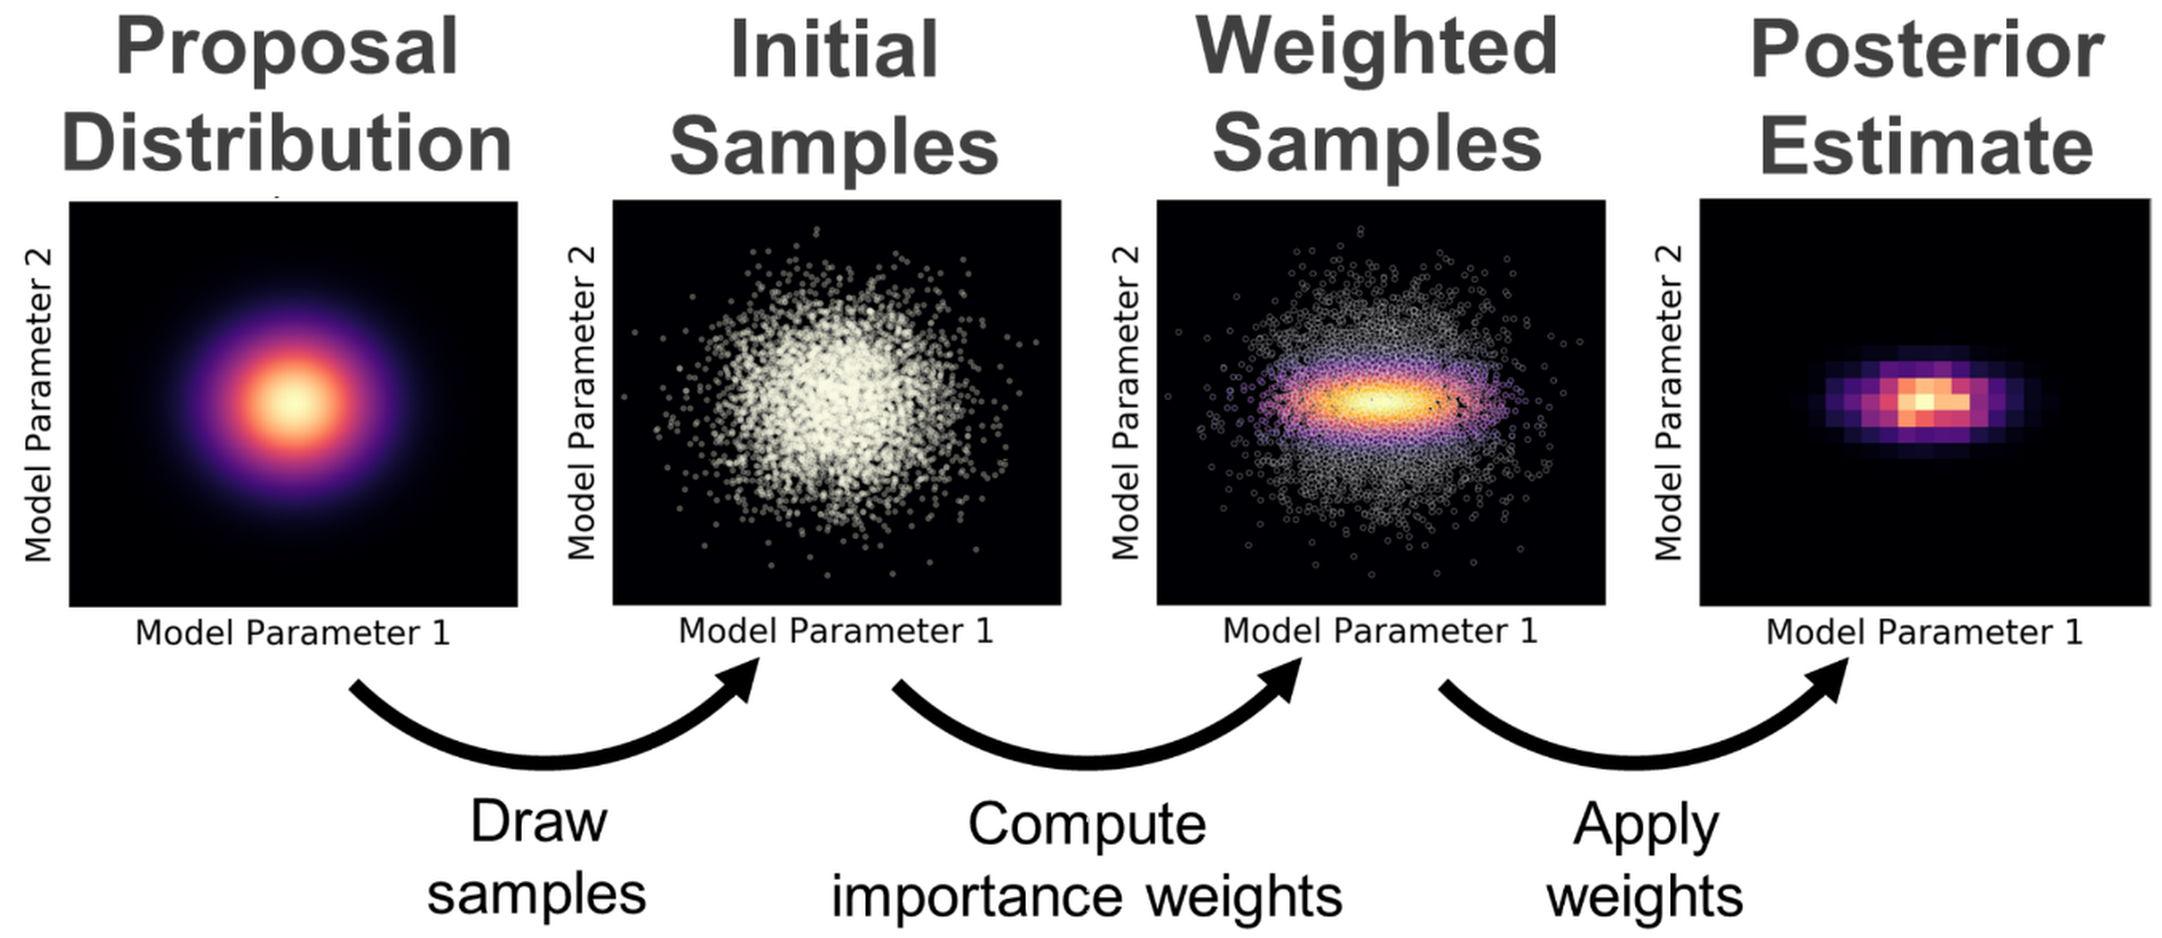
\includegraphics[scale=0.28]{Introduccion/Figures/Figura MCMC Pesos Muestreo.png}
	\caption{Esquema del \textit{muestreo de importancia}, una técnica para
	generar muestras de una distribución propuesta como estimación inicial (a
	priori) $\mathcal{Q}(\mathbf{\Theta})$ que se muestra en la primera gráfica.
	Se emplea un algoritmo para proponer muestras del espacio de parámetros que
	aceptar o rechazar (cuyas muestras realizadas para este ejemplo se pueden
	ver en la segunda gráfica), con la finalidad de estimar la distribución
	posterior vista en la última gráfica. Figura obtenida de
	\citeyearparen{speagle_conceptual_intro_mcmc_2020}.}
	\label{figuraMcmcMuestreoImportancia}
\end{figure}

\subsubsection{\code{emcee}: MCMC en Python} \label{intro:phoebe:problema_inverso:muestreo:emcee}

Las \textbf{cadenas de Markov de Monte Carlo} (conocidas por sus siglas en
inglés \textbf{MCMC}) generan muestras de la distribución a priori formando
\textit{cadenas} de valores del vector de parámetros $\mathbf{\Theta}$
correlacionados. Cada valor muestreado se adjunta a la cadena; después de $n$
iteraciones se calcula la \textit{densidad} $\rho(\mathbf{\Theta_i})$ de las
muestras dentro de una región $\delta_{\mathbf{\Theta}}$ centrada en el vector
$\mathbf{\Theta}_i$, definida por el número de muestras dentro de la región de
interés $m(\mathbf{\Theta_i})$:

\begin{eqfloat}[!ht]
	\centering
	\begin{equation}
		\rho(\mathbf{\Theta}) \equiv \frac{m(\mathbf{\Theta})}{n}
	\end{equation}
\end{eqfloat}

Dadas suficientes iteraciones, la densidad $\rho(\mathbf{\Theta})$ estará
distribuida de la misma forma que la distribución posterior
$\mathcal{P}(\mathbf{\Theta})$; esto se puede integrar para llegar al
\textit{valor esperado} de la distribución posterior, la cual es definida como:

\begin{eqfloat}[!ht]
	\centering
	\begin{equation}
		\mathbb{E}_{\mathcal{P}}\left[f(\mathbf{\Theta})\right] = \int{f(\mathbf{\Theta}) \mathcal{P}(\mathbf{\Theta}) \textrm{d}\mathbf{\Theta}}
	\end{equation}
\end{eqfloat}

Esta integral se puede expresar como una sumatoria como es visto en \citeyearparen{speagle_conceptual_intro_mcmc_2020}, donde $f_i(\mathbf{\Theta})
\equiv f_i$ son muestras del espacio de parámetros tomadas de tal manera que
cada muestra se considera \textit{independiente} e \textit{idénticamente
distribuida} (\textbf{IID} por sus siglas en inglés) tras $n$ iteraciones:

\begin{eqfloat}[!ht]
	\centering
	\begin{equation}
		\mathbb{E}_{\mathcal{P}}\left[f(\mathbf{\Theta})\right] = n^{-1} \sum_{i=1}^{n}{f_i}
	\end{equation}
\end{eqfloat}

Donde el peso de cada muestra se toma como $1/n$ debido a que las muestras se
consideran IID. El proceso de generar cada muestra en la cadena de Markov
consiste de un algoritmo probabilístico que solo depende de la muestra anterior;
el algoritmo de \textbf{Metropolis-Hastings} descrito en en
\citeyearparen{mackay_information_theory_inference_learning_algorithms_2003}
adopta una muestra propuesta $\mathbf{\Theta}^*$ bajo la siguiente condición:

\begin{eqfloat}[!ht]
	\centering
	\begin{equation}
		a = \frac{\tilde{\mathcal{P}}(\mathbf{\Theta}')}{\tilde{\mathcal{P}}(\mathbf{\Theta})} \frac{\mathcal{Q}(\mathbf{\Theta} ; \mathbf{\Theta}')}{\mathcal{Q}(\mathbf{\Theta}' ; \mathbf{\Theta})}
	\end{equation}
\end{eqfloat}

Donde $\tilde{\mathcal{P}}/\mathcal{Z} = \mathcal{P}$ representa la función de
densidad posterior no normalizada (antes de dividir por la evidencia
$\mathcal{Z}$ para llegar a la función de densidad de probabilidad
$\mathcal{P}$), y $\mathcal{Q}(\mathbf{\Theta}_1 ; \mathbf{\Theta}_2)$
representa la función de densidad de propuestas, la cual calcula la probabilidad
de obtener una nueva muestra $\mathbf{\Theta}'$ dada la muestra/posición actual
$\mathbf{\Theta}$. El factor $a$ representa la probabilidad de aceptar la nueva
muestra $\mathbf{\Theta}'$: si $a \geq 1$, entonces se toma $\mathbf{\Theta}'$
como la nueva posición de la cadena. Si $a <1$, se acepta la nueva muestra con
una probabilidad de $a$; en el caso de ser rechazada, la cadena se mantiene en
su posición actual $\mathbf{\Theta}$, a partir de donde el proceso empieza de
nuevo para la siguiente iteración. Este algoritmo trabaja bajo la suposición que
se puede calcular el valor de $\tilde{\mathcal{P}}$ para un valor dado de
$\mathbf{\Theta}$; al dejar correr la cadena por $n$ iteraciones se encuentra
que la densidad del espacio de parámetros $\rho(\mathbf{\Theta})$ converge con
$n \rightarrow \infty$.

En Python existe la librería
\code{emcee}\footnote{\url{https://emcee.readthedocs.io/en/stable/}}, una
implementación de MCMC haciendo uso de ensambles de cadenas de Markov e
invarianza de transformaciones afines para generar cadenas de muestras con un
tiempo menor de convergencia a la solución final. \code{emcee} implementa un
algoritmo denominado el \textit{stretch move}, descrito en
\citeyearparen{goodman_ensemble_samplers_affine_invariance_gw10_stretch_move_2010},
en donde la nueva posición de una cadena depende de otra cadena en el ensamble $S =
{X_k}$, para $k$ caminadores $X \in {X_1, X_2, ..., X_k}$. Dado un caminador
$X_k$, primero se toma otro caminador del ensamble complementario $S_{[k]} =
{X_j, j \neq k}$ del cual proponer una nueva posición $Y$:

% TODO: formatting new page
\newpage

\begin{eqfloat}[!ht]
	\centering
	\begin{equation}
		(X_{k}(t) \rightarrow Y) = X_j + Z[X_{k}(t) - X_j]
	\end{equation}
\end{eqfloat}

Donde $Z$ es un valor aleatorio muestreado de una distribución $g(z = Z)$:

\begin{eqfloat}[!ht]
	\centering
	\begin{equation}
		g(z) \propto \left\{\begin{matrix}
			\frac{1}{z} & | \ z \in \mathrm{Cond}(z) \\
			0 &| \ z \notin \mathrm{Cond}(z) \\
			\end{matrix}\right.
	\end{equation}
\end{eqfloat}

Donde se define el conjunto $\mathrm{Cond}(z) = [1/c, c]$ dado un valor $c$;
\citeyearparen{goodman_ensemble_samplers_affine_invariance_gw10_stretch_move_2010}
dan un valor de $c = 2$, pero en principio es un parámetro ajustable del
algoritmo para obtener mejores resultados según el problema en cuestión. Una vez
obtenido una nueva posición se evalúa con un criterio parecido a aquel
implementado en el algoritmo de Metropolis-Hastings:

\begin{eqfloat}[!ht]
	\centering
	\begin{equation}
		q = Z^{(N - 1)} \left(\frac{\tilde{\mathcal{P}}(\mathbf{\Theta}_Y)}{\tilde{\mathcal{P}}(\mathbf{\Theta}_X)}\right)
	\end{equation}
\end{eqfloat}

Donde $\mathbf{\Theta}_Y$ y $\mathbf{\Theta}_X$ corresponden al vector de
parámetros de los caminadores $Y$ y $X$ respectivamente. La nueva posición solo
es aceptada si $q \geq 1$, de lo contrario el caminador permanece en su posición
actual $Y = X_{k}(t + 1) = X_{k}(t)$. Dado a que cada nuevo valor en la cadena
de un caminador depende del estado actual del resto del ensamble, este problema
es inherentemente serial; para poder actualizar a más de un caminador a la vez
se divide el ensamble $S$ en 2 subconjuntos $S^{(1)} = \{ X_k; k = 1, 2, ...,
K/2 \}$ y $S^{(2)} = \{ X_k; k = (K/2) + 1, ..., K \}$ para un ensamble total
compuesto de $K$ caminadores. Esto permite actualizar la posición de todos los
caminadores en un subconjunto $S^{(1)}$ o $S^{(2)}$ simultáneamente usando los
caminadores en el subconjunto opuesto para proponer su nueva posición.
\citeyearparen{foreman-mackey_emcee_2013} describen el proceso a mayor detalle,
mientras que la implementación se puede ver en su repositorio de
GitHub\footnote{\url{https://github.com/dfm/emcee}}.

\subsubsection{MCMC en PHOEBE}

El problema de un sistema binario estelar es uno de alta dimensionalidad debido
a la cantidad de parámetros libres. Al momento de explorar el espacio de
parámetros la distribución de densidad posterior tiende a estar concentrada en
pequeños volúmenes de cuboides de $N$ dimensiones; el volumen crece a una alta
tasa a comparación con el área superficial del cuboide. Esto presenta una
situación problemática para un proceso de MCMC, en donde una mayor razón de las
posiciones propuestas para cada caminador es rechazada por la mayor diferencia
entre los valores resultantes de la función $\tilde{\mathcal{P}}$. El volumen de
un cuboide de $N$ dimensiones con lados de largo $l$ se obtiene mediante la
siguiente ecuación:

\begin{eqfloat}[!ht]
	\centering
	\begin{equation}
		V(l) = \prod_{i = 1}^{N}{l} = l^N
	\end{equation}
\end{eqfloat}

Esta baja tasa de pasos aceptados causa un largo \textit{tiempo de
autocorrelación}, el cual describe el número de iteraciones necesarios para que
una cadena \quotes{olvide} su posición inicial. El tiempo de autocorrelación
parametriza la cantidad de muestras independientes en el ensamble de cadenas;
por lo tanto el número de muestras independientes está dado por el número de
iteraciones totales corridos en el muestreo dividido por el tiempo de
autocorrelación. Para problemas como el modelado de un sistema binario en
PHOEBE, este problema se puede mitigar con el uso de una mayor cantidad de
caminadores (en el orden de cientos de caminadores) y el uso de una distribución
adecuada de muestreo inicial.\

Para correr un muestreo de parámetros en PHOEBE simplemente se necesita crear un
nuevo resolvedor (\textit{solver} en la API de PHOEBE) del tipo \code{emcee}, en
el cual se especifican las características del ensamble. Esto se puede ver en la
\refcode{codigoMuestreoMCMC}.

\begin{figure}[!ht]
	\centering
	\begin{lstlisting}[language=Python, autogobble]
		b.add_solver('sampler.emcee', solver='mcmc_sampler',
			init_from=['mcmc_prior'], 
			niters=5000, nwalkers=200, 
			progress_every_niters=5)
	\end{lstlisting}
	\caption{Resolvedor de tipo \code{emcee} para muestrear el espacio de
	parámetros dado el bundle \code{b}. Este muestreo está configurado para
	correr 5000 iteraciones con 200 caminadores; al contrario de un optimizador,
	el muestreo de \code{emcee} no tiene manera de saber si ha convergido a una
	solución para determinar cuando ha obtenido suficientes muestras. Por
	seguridad, se puede configurar para que el muestreo guarde su progreso
	después de cada \code{progress\_every\_niters} iteraciones, el cual se puede
	utilizar para revisar el progreso del muestreo o para continuar un proceso
	que haya terminado de manera prematura (por ejemplo, en el caso de una falla
	en el equipo).}
	\label{codigoMuestreoMCMC}
\end{figure}

El resolvedor \code{emcee} creado usará los conjuntos de datos\textemdash
\textit{datasets} en PHOEBE\textemdash habilitados para evaluar la función de
costo para cada vector de parámetros muestreado. En vez de especificar
explícitamente los parámetros que muestrear, el resolvedor toma de entrada el
parámetro \code{init\_from}, el cual representa el conjunto de distribuciones
propuestas $\mathcal{Q}(\mathbf{\Theta})$ para los parámetros que muestrear.
Estos son distribuciones de forma arbitraria; para facilitar su creación y
maximizar la facilidad de tomar muestras discretas PHOEBE ofrece la habilidad de
crear distribuciones informativas (de forma de Gaussianas) o no-informativas
(distribuciones uniformes limitadas a cierto rango) alrededor de los valores
actuales de los parámetros en el bundle visto en la \refcode{codigoMuestreoPriors}.

\begin{figure}[!ht]
	\centering
	\begin{lstlisting}[language=Python, autogobble]
		b.add_distribution({
			'asini@orbit': phoebe.gaussian_around(0.5),
			'q': phoebe.gaussian_around(0.1),
			'vgamma@system': phoebe.gaussian_around(5.0),
			'ecc@orbit': phoebe.gaussian_around(0.05),
			'per0@orbit': phoebe.gaussian_around(10.0)
		}, distribution='ndg', overwrite_all=True)

		b.add_distribution({
			'asini@orbit': phoebe.uniform_around(2),
			'q': phoebe.uniform_around(0.5),
			'vgamma@system': phoebe.uniform_around(15.0),
			'ecc@orbit': phoebe.uniform_around(0.2),
			'per0@orbit': phoebe.uniform_around(20.0)
		}, distribution='nuni', overwrite_all=True)
	\end{lstlisting}
	\caption{Creando dos distribuciones por separado para iniciar como punto de
	partida para un muestreo de MCMC en PHOEBE dado un bundle \code{b} cuyos
	valores han sido previamente optimizados para llegar a un ajuste adecuado.
	La distribución \code{ndg} representa una Gaussiana multi-dimensional,
	especificando el valor de $\sigma$ para cada parámetro como valor de entrada
	a la función \code{phoebe.gaussian\_around}. La distribución \code{nuni}
	representa una distribución multi-dimensional uniforme, donde el valor de
	entrada a la función \code{phoebe.uniform\_around} representa la anchura
	total de la distribución de densidad de cada parámetro. La representación
	gráfica de estas distribuciones se puede ver en la
	\reffigure{figuraPhoebeMuestreoPriors}}
	\label{codigoMuestreoPriors}
\end{figure}

\begin{figure}[!ht]
	\centering
	\xincludegraphics[scale=0.36, label=\textbf{(a)}, labelbox=true, pos=ne, fontsize=\Large]{Introduccion/Figures/Figura PHOEBE Priors Gaussian.png}
	\xincludegraphics[scale=0.36, label=\textbf{(b)}, labelbox=true, pos=ne, fontsize=\Large]{Introduccion/Figures/Figura PHOEBE Priors Uniform.png}
	\caption{Gráfica mostrando las distribuciones creadas por el código en la
	\refcode{codigoMuestreoPriors}. Este \textit{corner plot} (su nombre en
	inglés) permite ver las distribuciones de los parámetros individuales en el
	último cuadro de cada gráfica, al igual que ver las correlaciones entre cada
	par de parámetros representada por cada intersección de una columna y un
	renglón. \textbf{(a)} representa la distribución normal multivariada
	\code{ndg}, mientras que \textbf{(b)} muestra la distribución uniforme
	\code{nuni}.}
	\label{figuraPhoebeMuestreoPriors}
\end{figure}

Un muestreo ideal convergerá a una distribución de densidad que se asemejará a
la distribución de probabilidad posterior de cada parámetro. De estas
distribuciones posteriores se pueden determinar los valores promedios e
incertidumbres (por ejemplo, en el caso de que sea una Gaussiana, el valor
promedio y la incertidumbre son triviales de obtener tras un ajuste analítico de
las muestras individuales, cosa que PHOEBE lo hace en automático) de cada
parámetro, al igual que identificar correlaciones entre distintos parámetros del
modelo. En dado caso que el muestreo corrido no haya sido suficiente (no haya
convergido, ciertos caminadores se quedaron \quotes{atascados} en una región del
espacio de parámetros, etc.) es posible continuar el resolvedor actual
utilizando el parámetro del resolvedor \code{continue\_from} para apuntar a la
solución producida por el resolvedor, o es posible crear un nuevo resolvedor de
tipo \code{sampler.emcee} cuyas distribuciones a priori sean la distribución de
densidad producida por el muestreo previo. Información adicional del API de
PHOEBE se ubica en su página de
documentación\footnote{\url{http://phoebe-project.org/docs/2.4/tutorials/emcee}}.
El muestreo empleado para este trabajo de tesis se encuentra en el
\refthesischapter{metodologia:modelocomputacional}.
% \subsection*{Variables Cataclísmicas}
\sout{Las variables cataclísmicas (CVs) son un tipo de sistemas binarios, compuestos
de una estrella enana blanca y una estrella de secuencia principal.}
% TODO: REMOVE ABOVE

Este tipo de sistemas muestran comportamiento variable a lo largo del tiempo, en
donde varía su luminosidad, espectro emitido, y otras propiedades del sistema.
No todas las variables cataclísmicas demuestran un comportamiento uniforme; sus
periodos de intensa actividad y el subsecuente periodo de atenuación pueden
variar en su duración y su magnitud. El mecanismo que genera esta variación se
les conoce como \textit{novae}; estos estallidos ocurren debido a la interacción
de las estrellas dentro del sistema.
\subsection*{Composición de las VCs}
La composición de las estrellas puede variar de un sistema a otro, pero en
general adhieren a los siguientes parámetros: una estrella enana blanca -
conocida como la estrella principal - y una estrella de secuencia principal
menos densa - la estrella secundaria. Esta estrella secundaria es más roja que
la principal; su espectro de emisión tiende a la región roja, llegando hasta el
infra-rojo en ciertos casos. Tomando en cuenta el sistema completo, se puede
observar en la distribución de variables cataclísmicas en el diagrama
Hertzsprung-Russell que la mayoría reside entre las regiones de enanas blancas y
la secuencia principal dependiendo de la contribución relativa de sus estrellas
componentes. \citet{disentanglingGaiaHR} No siempre ocurre algún tipo de
interacción entre las estrellas componentes dentro del sistema; esto va a
depender de los volúmenes de las estrellas y la distancia entre ellas, ya que la
manera principal en que interactúan entre si es en base a su atracción
gravitacional. Entre más cerca de una a otra las fuerzas gravitacionales
empiezan a distorsionar la secundaria hasta tener una forma más plana y menos
uniforme. Este volumen, llamado el lóbulo de Roche, es la región de espacio en
donde la estrella puede mantener a su material atrapada por su gravedad. En un
sistema binario cada estrella tiene un lóbulo de Roche definido, los cuales
están en contacto uno con el otro. Un ejemplo simple se puede ver en la figura
\ref{acrecionSmithReview}, donde la estrella secundaria ha llenado su volumen y
su material empieza a caer hacia la enana blanca debido a su atracción
gravitacional. \\\newline
Al cruzar el lóbulo de Roche de la estrella secundaria, la materia perdida no
puede caer directo a la superficie de la enana blanca a ser absorbida
inmediatamente. Esto se debe al momento angular de las estrellas, tanto por su
rotación como su órbita alrededor de su estrella compañera. Por lo tanto, al
cruzar el punto de contacto entre los lóbulos (este conocido como el punto
Lagrangiano L1) el material tiene una componente de velocidad tangente a la
dirección a la enana blanca. A lo largo de que el material se empieza a acumular
toma una forma dependiendo de las propiedades magnéticas de la enana blanca. En
un sistema donde no ejerce un efecto significativo un campo magnético, el
material forma un \textit{disco de acreción} alrededor de la enana blanca. Este
disco se concentra en el ecuador de esta misma estrella, el cual empieza a
emitir radiación en forma de líneas de emisión. Al contrario en un sistema
magnético (llamados \textit{variables cataclísmicas magnéticas} o
\textit{polares}) donde el campo magnético de la enana blanca es significativo
el material no logra acumularse en un solo disco. Este material debido a ser un
plasma ionizado tiene una carga eléctrica intrínseca, la cual la permite ser
guiada por el campo magnético de la enana blanca a su destino final al polo
magnético de esta misma estrella. \\\newline
\begin{figure}
	\centering
	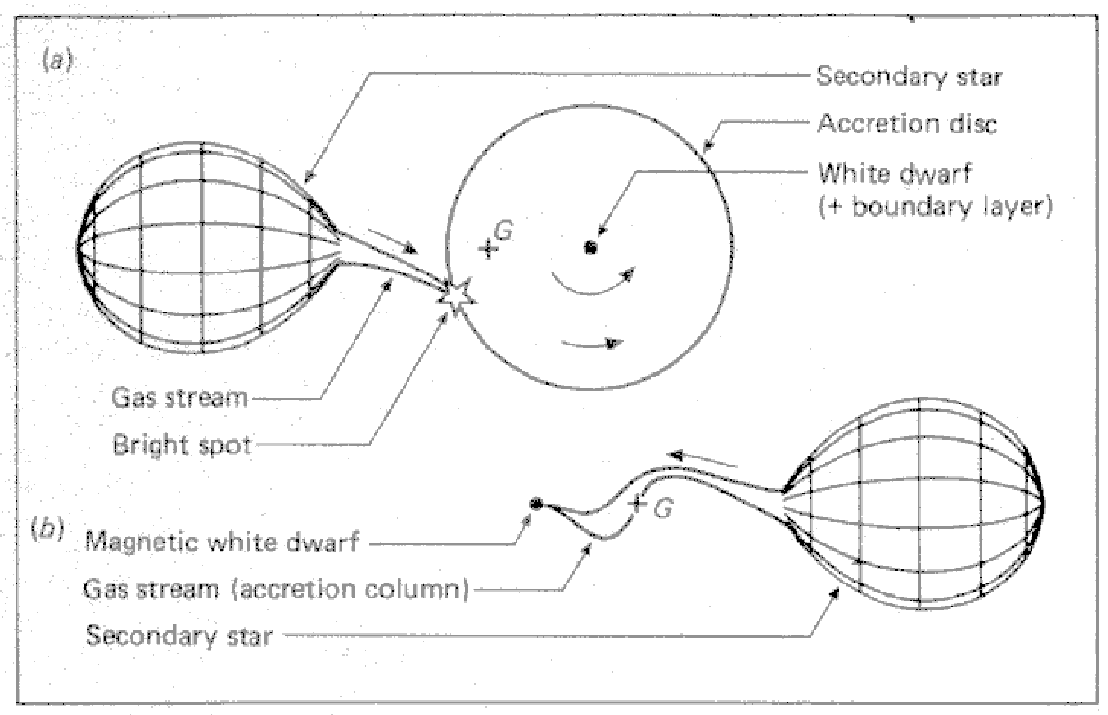
\includegraphics[scale=0.4]{Introduccion/Figures/Figura Acrecion_SmithReview.png}
	\caption{Diagrama de una estrella enana blanca absorbiendo material de su
	compañera estrella de secuencia principal por medio de la interacción de sus
	lóbulos de Roche.} \cite*{smithReview}
	\label{acrecionSmithReview}
\end{figure}

Todas las variables cataclísmicas han obtenido su nombre debido a sus cambios
rápidos en sus propiedades durante periodos de observación. El mecanismo
principal que causa estas variaciones se debe a los estallidos periódicos,
conocidos como \textit{novae}. Al igual como no todos los sistemas muestran las
mismas propiedades en sus componentes existen diferentes tipos de estallidos:
\textit{novae clásicos}, \textit{novae enanos}, y \textit{nova-like}.
\cite*{smithReview} \\\newline
Los novae clásicos son aquellos estallidos observados en sistemas binarios que
causa que su luminosidad aumente por varias magnitudes en una escala de tiempo
relativamente corta (puede ser en la escala de días hasta meses).
\cite*{smithReview} Aparte de la radiación generada debido a reacciones
termonucleares, los novae expulsan un entorno de gas caliente a grandes
velocidades, llegando a miles de kilómetros por segundo. Pocos sistemas binarios
muestran nova recurrentes a lo largo del tiempo en intervalos de decenas o
cientos de años; la mayoría ha mostrado un solo estallido en su tiempo de
observación. En sistemas no magnéticos, el disco de acreción sirve como el motor
principal de estos estallidos. La mayoría del material en el disco es hidrógeno;
este crea una capa en la superficie de la enana blanca. A lo largo de lo que se
acumula este material aumente su grosor, aumentando la temperatura de la capa.
Este aumento de temperatura causa que la presión en esta capa alcance un punto
en donde empiezan a ocurrir reacciones termonucleares de parte del hidrógeno
presente en esta capa.
% \subsection{Enana Blanca}\label{intro:sec:EnanaBlanca}

Una estrella nace de una nube molecular interestelar, una región de material
ubicada en el espacio entre estrellas. Dependiendo de la masa inicial de el
conjunto inicial de material es lo que determina las fases que la estrella pasa
al envejecer. El camino que tomaría una estrella de secuencia principal durante
el fin de su vida se puede ver en la figura \ref{evolucionMSEstrella}, donde
está marcado los distintos caminos que una estrella toma en el \textbf{diagrama
Hertzsprung-Russell (HR)}. Este diagrama relaciona la temperatura efectiva de la
estrella con su luminosidad, dada en términos de luminosidad solar.

\begin{figure}[!ht]
	\centering
	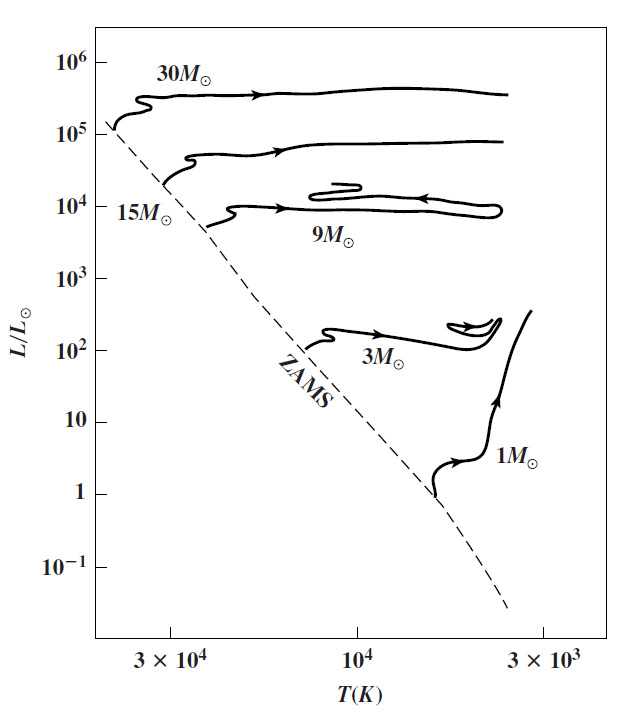
\includegraphics[scale=0.5]{Introduccion/Figures/Figura Evolucion_MS_Astronomy_Physical_Perspective.png}
	\caption{Evolución de estrellas de la secuencia principal basado en su masa
	inicial en el diagrama HR. La línea punteada representa la posición de la
	estrella en el primer momento que se integra a la secuencia principal. Al
	consumir el hidrógeno en su núcleo por las reacciones nucleares que ocurren
	en esta misma región se comienza a desatar el equilibrio delicado que
	mantiene la forma de la estrella. Esta deformación provoca una oscilación en
	su tamaño, causado por las fluctuaciones del balance entre la presión
	radiativa generada por las reacciones nucleares en el núcleo contra la
	presión gravitacional.}
	\citet{astronomyPhysicalPerspective_stellarOldAgeChapter}
	\label{evolucionMSEstrella}
\end{figure}

Aquellas estrellas cuyas masas iniciales recae bajo 8.5-10.6 \(M_{\odot}\)
terminan su vida como una estrella \textit{enana blanca.}
\citet*{whiteDwarfsReview} El ciclo de reacciones nucleares dentro del núcleo de
una estrella solo ocurre en la presencia de cierta cantidad de hidrógeno durante
su tiempo en la secuencia principal; al acabarse esta fuente de combustible la
estrella empieza a colapsar en si misma, ya que la presión radiativa del núcleo
hacia el exterior disminuye a tal grado que la presión hacia el interior de su
propia gravedad causa el encogimiento de la estrella. Esta disminución de su
radio causa que el núcleo se caliente hasta llegar a temperaturas \(T \approx
10^{8} K\) [\citet*{astronomyPhysicalPerspective_stellarOldAgeChapter}],
empezando de nuevo reacciones nucleares, esta vez involucrando el helio en vez
del hidrógeno. Estas reacciones se conocen como el proceso \textit{triple alfa},
donde tres partículas alfa \(^{4}He\) fusionan para crear un átomo de \(^{12}C\)
y un fotón gama. Mientras que en el núcleo ocurren reacciones con elementos cada
vez más pesados, el resto de los elementos más livianos (ya sea hidrógeno en el
caso de estrellas sometidas al proceso alfa u objetos más pesados como neon u
oxígeno en el caso de núcleos más densos
\citet*{astronomyPhysicalPerspective_stellarOldAgeChapter}) siguen presentes en
las capas que rodean al núcleo. La energía generada por las reacciones nucleares
dentro del núcleo se transporta a estas capas externas por medio de la radiación
generada, la cual calienta los elementos livianos, desatando de nuevo la fusión
de elementos como hidrógeno. Estas explosiones en las capas exteriores de la
estrella causa la expansión de la estrella, llegando a la fase gigante dentro
del diagrama HR.

Dependiendo de su masa inicial, una estrella puede seguir produciendo elementos
cada vez más pesados dentro de su núcleo. Sin embargo, este combustible solo le
permite a la estrella llegar hasta cierta temperatura, a partir de cual no podrá
seguir manteniendo su tasa de fusión nuclear. Una vez que llegue a este punto
empieza a expulsar las capas exteriores hasta solo dejar el núcleo expuesto,
ahora inerte debido a la ausencia de fusión nuclear. Este resto de la estrella
progenitora es lo que se conoce como la \textit{enana blanca}, a pesar de no ser
una estrella formalmente. La composición del material dentro de este objeto es
distinto al de una estrella de secuencia principal; a pesar de tener como mínimo
una masa \textapproxtilde 0.30-0.45 \(M_{\odot}\) su radio en promedio cae
dentro del mismo orden de magnitud que el radio de la Tierra.
\citet*{whiteDwarfsReview} Esto implica una densidad inmensa, en donde solo un
\textit{gas degenerado de Fermi} puede existir en estas condiciones. Un gas
degenerado surge como consecuencia del \textbf{principio de exclusión de Pauli}:
dentro de una molécula no pueden existir más de un electrón por cada estado
cuántico. Es debido a éste fenómeno que las moléculas de una estrella enana
blanca están acumuladas en un volumen varias ordenes menor comparado con una
estrella de secuencia principal, en la cual los electrones degenerados les
permiten a las moléculas almacenar más energía térmica de lo que predicen los
modelos en un gas no degenerado. Por lo tanto la escala termodinámica de una
estrella enana blanca puede llegar a ordenes de \textapproxtilde \(10^{10}\)
años, en la cual su temperatura efectiva podría disminuir de \(100,000 K\) a
\textapproxtilde \(5,000 K\). \citet*{whiteDwarfsReview}
% \section{Enana Roja} \label{intro:sec:EnanaRoja}
\part{Muestra}

% TODO: make abstract

% Este trabajo tiene como objetivo principal producir datos fotométricos de
% estrellas marcadas como candidatas a variables cataclísmicas. Debido a la
% escasez de variables cataclísmicas en la literatura---solo 1093 variables
% cataclísmicas habían sido identificadas hasta 2015 en el catálogo de Ritter-Kolb
% \citet*{ritterKolbImpactArticle}---existen pocos datos con los cuales corroborar
% los modelos actuales de una variable cataclísmica. Al identificar nuevas
% estrellas como variables cataclísmicas y generar una curva de luz de estas
% mismas estaremos aportando a la muestra disponible en la literatura. Con este
% fín utilizamos el catálogo de \gaia para obtener nuestras candidatas, usando el
% catálogo de SDSS para seleccionar solo las fuentes no observadas previamente. 

\chapter{Catálogos}

\section{Gaia} \label{muestra:sec:gaia}

Originalmente denominado como \textit{GAIA}, la misión de \gaia fue lanzada por
la \textbf{Agencia Espacial Europea (ESA)} el 19 de Diciembre del 2013, con el
objetivo de generar un mapa tridimensional de nuestra Galaxia, la Vía Láctea.
Esto incluye calcular las propiedades astrométricas y astrofísicas de sus
fuentes observadas con mayor precisión que cualquier otro catálogo publicado
previamente. Para lograr esto se utiliza un satélite espacial, el cual está
denominado como \gaiaNoSpace, ubicado en el punto de Lagrange L2 con respecto al
sistema Sol-Tierra. Desde este punto la nave tiene una vista sin obstrucciones
que le permite observar una cantidad de estrellas enorme, con \textapproxtilde
1,000 millones de fuentes visibles con los instrumentos del satélite
\gaiaNoSpace. \autocite{gaiaMission}

\subsection{Fotometría}

\subsection{Data Release 2} \label{muestra:sec:gaia:dr2}

Para facilitar el acceso público a los datos recabados por la misión de \gaia la
ESA ha escogido liberar los datos públicamente mediante los van recibiendo y
procesando. Estos son conocidos como los \textbf{Data Releases}. Este trabajo se
basa en el \textbf{Data Release 2}, el cuál de ahora en adelante será denominado
simplemente \textbf{GDR2}. Este catálogo está compuesto de las observaciones
hechas por \gaia entre las fechas de 25 de Julio del 2014 y el 23 de Mayo del
2016, un periodo de tiempo de 22 meses en total. \autocite{gaiaDr2} GDR2 consiste
de \num{1692919135} de fuentes individuales. Existe una gran diversidad de objetos
dentro de este catálogo, desde estrellas de secuencia principal, asteroides
dentro del sistema solar, hasta estrellas variables en las regiones más lejanas
en la Galaxia.

Los datos utilizados en este estudio fueron accedidos a través de el
\textit{Gaia Archive}\footnote{\url{https://gea.esac.esa.int/archive/}}, una
herramienta libre publicada por la ESA. Este cuenta con una interfaz de
ADQL\footnote{\url{https://www.ivoa.net/documents/ADQL/20180112/PR-ADQL-2.1-20180112.html}},
un lenguaje estructurado para hacer consultas a la base de datos de
\gaiaNoSpace, incluyendo tablas conectando los datos de \gaia con otros
catálogos, por ejemplo el catálogo de SDSS.

\section{Sloan Digital Sky Survey}

La colección de catálogos \textbf{Sloan Digital Sky
Survey}\footnote{\url{https://www.sdss.org}} (de ahora en adelante será referido
como \textbf{SDSS}) compila varias fuentes de datos astronómicos y astrofísicos
en un sitio centralizado, con el objetivo de crear un mapa tridimensional del
Universo con una precisión no vista antes. Estos incluyen imágenes de objetos
astronómicos en varios colores, acompañados de un espectro obtenido como parte
de esta misión. Para los finales del siglo XX habían surgido avances
tecnológicos que llegarían a revolucionar la astronomía observacional. De estos,
los de mayor interés ocurrieron con los detectores de estado sólido y en la
capacidad computacional de procesamiento. Partiendo de estos empezaron a
desarrollar la infraestructura necesaria para recabar datos fotométricos y
espectroscópicos.

El instrumento principal utilizado es el telescopio de 2.5m, ubicado en el
observatorio \textit{Apache Point Observatory}, descrito a detalle en
\autocite{sdss2_5mTelescope}. Este telescopio de diseño de Ritchey-Chrétien
alimenta dos instrumentos separados; una CCD multi-banda de ancha área, y un par
de espectrógrafos alimentados por fibra óptica. Su construcción empezó en 1998,
pero no fue hasta el año 2000 que estuvo operacional.

\subsection{Data Release 9}

SDSS libera datos en colecciones iterativas; es decir cada Data Release (DR)
liberado contiene todas las observaciones que forman parte del DR previo,
agregando los datos recabados durante el periodo de observación para el DR
actual. Cada DR cae bajo una fase de operaciones de SDSS, delimitado tanto por
las fechas de observaciones como por los instrumentos y tipos de datos
disponibles. Para el periodo operacional de
\hyperref[muestra:sec:gaia:dr2]{GDR2} el catálogo más actual de SDSS era el DR9
publicado como parte de SDSS-III
\footnote{\url{https://www.sdss3.org/index.php}}. Esta tercera fase fue marcada
por una gran mejora del equipo espectroscópico, instalando nuevos instrumentos
con los cuales pudieron analizar la dinámica de nuestra Galaxia, al igual que
otras galaxias y planetas gaseosos extra-solares. 


\chapter{Selección de Objeto}

Este trabajo tiene como objetivo realizar una campaña de observación para un
sistema cuyos parámetros físicos no han sido determinados, con el propósito de
confirmar su estatus como variable cataclísmica o como una binaria eclipsante,
dependiendo del sistema y proponer una primera solución fotométrica del sistema.
Para esto, se implementó un proceso para separar e identificar objetos de
interés para observar desde el Observatorio Astronómico Universitario en
Iturbide. A continuación se describe los aspectos técnicos importantes de la
búsqueda. El código completo se encuentra en la carpeta
\href{https://github.com/KnightIV/UANL_MAPTA_Observaciones/tree/main/obsrv_plan}{\code{obsrv\_plan}},
cuyo punto de entrada se ubica en el script
\href{URLhttps://github.com/KnightIV/UANL_MAPTA_Observaciones/blob/main/obsrv_plan/main.py}{\code{main.py}}.

\section{Szkody et al. (2002): Cataclysmic Variables from the Sloan Digital Sky Survey} \label{muestra:szkody2002}

Con el lanzamiento del SDSS, Szkody y su equipo reconocieron una nueva área de
oportunidad para expandir la población de \textit{variables cataclísmicas} (VCs)
conocidas en la Galaxia. De interés particular son aquellos sistemas que más se
aproximan al periodo mínimo según los modelos evolutivos de las VCs; estos
objetos llegan a magnitudes fuera del alcance de la mayoría de los telescopios
usados hasta este entonces, por lo cual no han sido el objetivo de estudio en la
literatura. Partiendo de SDSS Szkody y colaboradores iniciaron una búsqueda de
VCs, con la expectativa de capturar una muestra representativa de
variables cataclísmicas en nuestra galaxia, en particular obteniendo muestras de
poblaciones históricamente imperceptibles a nuestros instrumentos.

Para restringir los sistemas que buscar, \citeyearparen{szkody2002CvSearchSdss}
aplicaron un criterio de color basado en el trabajo de
\citeyearparen{krisciunas1998SdssCriteria}, en el cual lograron determinar
concentraciones de diferentes tipos de objetos utilizando diagramas de
color-color. A pesar de haber hecho estas observaciones antes del año de
lanzamiento de SDSS, Krisciunas y colaboradores lograron obtener observaciones
utilizando equipo cuyas características se asemejan a las de los instrumentos
utilizados para SDSS. Partiendo de estos resultados, Szkody y colaboradores
determinaron los siguientes criterios en las regiones azules y rojas del
espectro:

\begin{equation}
	\begin{split}
		& u^* - g^* < 0.45 \\
		& g^* - r^* < 0.7 \\
		& r^* - i^* > 0.30 \\
		& i^* - z^* > 0.4
	\end{split}
	\label{muestra:szkody2002:criterioeqs}
\end{equation}

Una vez recabada la muestra de candidatas a observar, Szkody y colaboradores
confirmaron su estatus como variables cataclísmicas basado en los espectros
obtenidos del SDSS desde el \textit{Apache Point Observatory}. Estos datos los
complementaron con observaciones de espectroscopía con el telescopio de 3.5m en
el \textit{Apache Point Observatory} así como observaciones fotométricas utilizando el
telescopio de 0.76m en el \textit{Manastash Ridge Observatory} de la Universidad
de Washington. En total identificaron 22 sistemas como variables cataclísmicas,
incluyendo 3 objetos previamente estudiados e identificados como tal. Presentan
la concentración de los objetos en el diagrama color-color, vistos en la
\reffigure{szkody2002ColorColorVCs}. 

\begin{figure}[!ht]
	\centering
	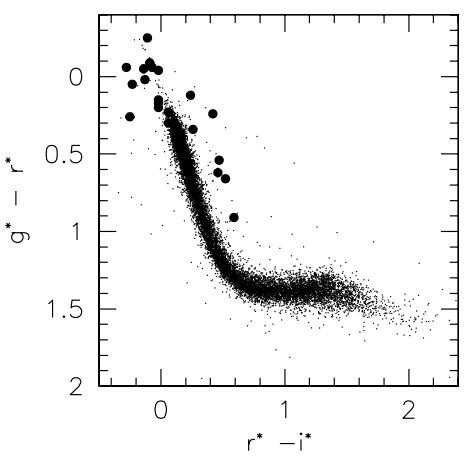
\includegraphics[scale=0.4]{Muestra/Secciones/Figures/gr-ri_Szkody2002.png}
	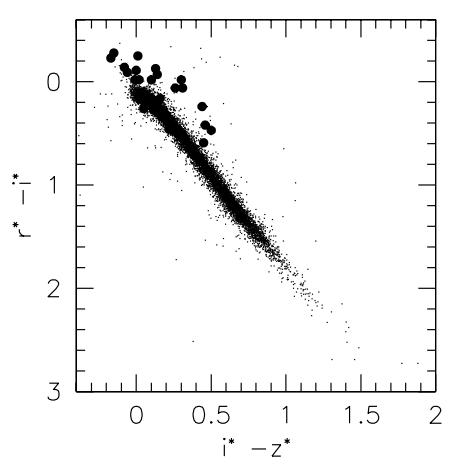
\includegraphics[scale=0.4]{Muestra/Secciones/Figures/ri-iz_Szkody2002.png}
	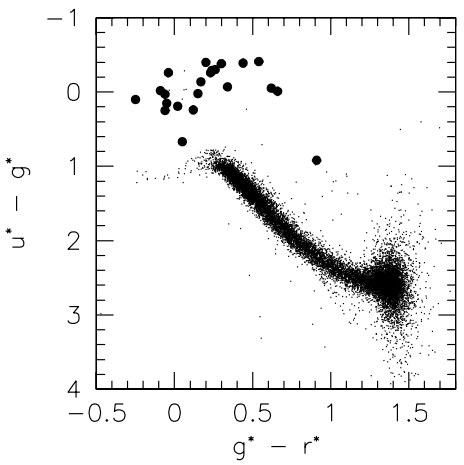
\includegraphics[scale=0.4]{Muestra/Secciones/Figures/ug-gr_Szkody2002.png}

	\caption{Variables cataclísmicas identificadas y observadas por Szkody y
		colaboradores (círculos negros fuertes). Se puede apreciar la separación
		de las variables cataclísmicas del locus estelar, vista en los puntos
		negros. \citeyearparen{szkody2002CvSearchSdss}}
	\label{szkody2002ColorColorVCs}
\end{figure}

\section{Búsqueda en Gaia}

Para obtener la muestra inicial de objetos de interés recurrimos a la base de
datos de Gaia. La selección de objetos fue llevada a cabo dentro del
\textit{Gaia Archive} utilizando su interfaz de ADQL. Los criterios
definidos por Szkody y colaboradores solo fueron definidos para el sistema
fotométrico de SDSS; para poder utilizar estos primero se llevó a cabo una
conversión de las magnitudes reportadas en el catálogo de Gaia a magnitudes en
los pasa bandas de SDSS. Esta conversión se llevó a cabo utilizando las
transformaciones definidas en la documentación de Gaia DR3
\citeyearparen{gdr3ReleaseDocumentation}, como se puede ver en la
\reffigure{gdr3SdssConversionGraphs}. Partiendo de estas magnitudes
transformadas se aplicó los criterios definidos en
\citeyearparen{szkody2002CvSearchSdss}. Sin embargo, solo dos de los 4 indices
de color se pudieron aplicar a la muestra de Gaia; no están definidas
transformaciones para las bandas $u$ ni $z$ de SDSS, ya que estas abarcan
longitudes de onda más extremas que las observadas por Gaia. El query de ADQL
ejecutada se puede encontrar en el apéndice \ref{apendice:gaiaAdql}. Se
obtuvieron en total más de \num{3630000} fuentes, el cual representa un 0.2\% de
los \num{1811709771} objetos reportados en el DR3 de Gaia. 

\begin{figure}[!ht]
	\centering
	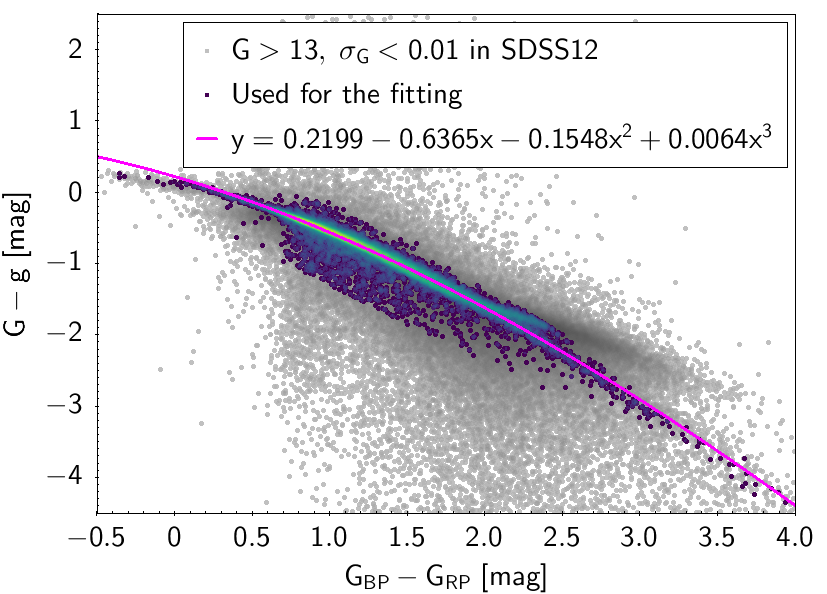
\includegraphics[scale=0.23]{Muestra/Secciones/Figures/Gaia-SDSS-Transform-g.png}
	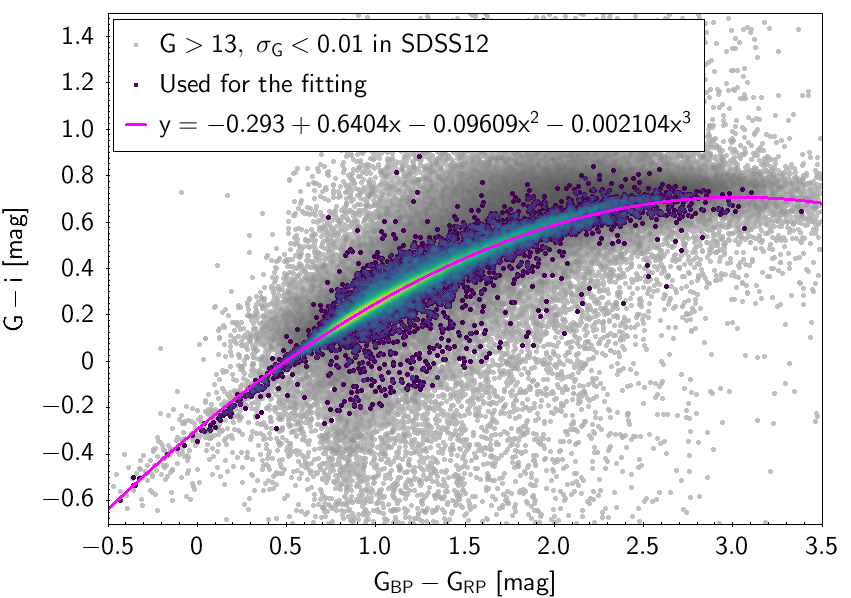
\includegraphics[scale=0.23]{Muestra/Secciones/Figures/Gaia-SDSS-Transform-i.png}
	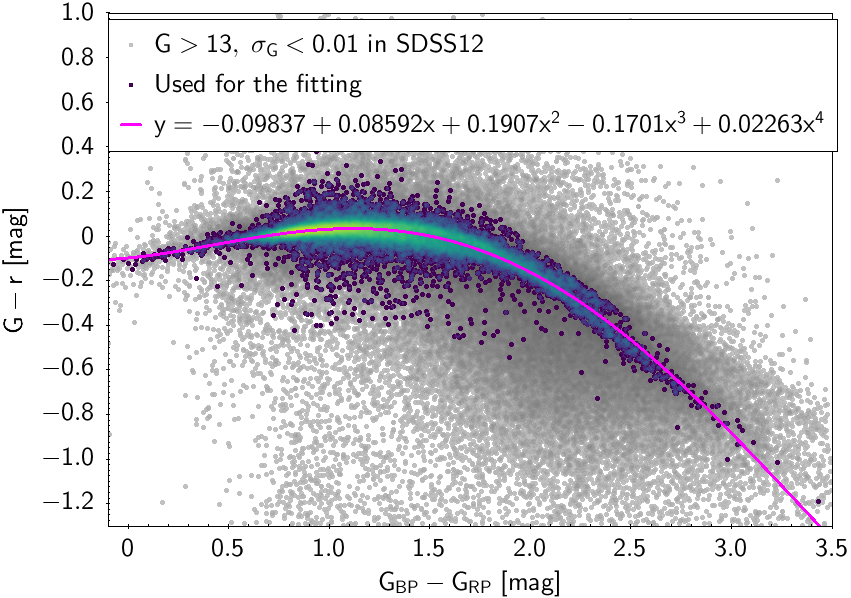
\includegraphics[scale=0.23]{Muestra/Secciones/Figures/Gaia-SDSS-Transform-r.png}

	\caption{Relación empírica entre las magnitudes reportadas en GDR3 y SDSS12.
	Las relaciones están dadas para 3 de las 5 bandas de SDSS12, debido a las
	diferencias entre las pasa bandas de Gaia y SDSS.
	(\citeyearparen{gdr3ReleaseDocumentation})}
	\label{gdr3SdssConversionGraphs}
\end{figure}

\section{Selección de Objetos Observables}

La ubicación en la bóveda celeste de un sistema candidata juega un papel
importante en la viabilidad de una campaña de observación desde el OAU. Esto
determina si un objeto es visible desde la locación geográfica del observatorio
durante las fechas de observación; de otra manera sería imposible apuntar un
telescopio al sistema. Para realizar esta tarea se utilizaron los módulos de
\code{astroplan} (\citeyearparen{astroplan}) y \code{astropy} (\citeyearparen{astropy}), aplicando
el algoritmo a los objetos resultados de la búsqueda en la base de datos de
Gaia. El código responsable se encuentra en el archivo
\href{https://github.com/KnightIV/UANL_MAPTA_Observaciones/blob/main/obsrv_plan/gaia/observable_targets.py}{\code{observable\_targets.py}}.

\section{Búsqueda en SIMBAD}

Una vez obtenidos los objetos de interés de la selección de objetos visibles se
utilizó la base de datos de
SIMBAD\footnote{\url{http://simbad.cds.unistra.fr/simbad/}}
(\citeyearparen{simbadDatabase}) para restringir los objetos de interés a un
tamaño manejable, con el objetivo de obtener un sistema clasificado como
variable cataclísmica, binaria eclipsante, o candidata a alguna de estas
clasificaciones. Uno de los objetivos de este trabajo de tesis fue realizar una
campaña de observación al sistema elegido, con finalidad de obtener una curva de
luz fotométrica; por lo tanto, un requisito para este trabajo de maestría es que
este sistema sea uno con una cantidad minima de estudios antecedentes; el
estudio del sistema dependerá en gran parte de la curva de luz obtenida de las
observaciones. El código que llevó a cabo esta búsqueda se encuentra en
\href{https://github.com/KnightIV/UANL_MAPTA_Observaciones/blob/main/obsrv_plan/simbad/categorize_all_targets.ipynb}{\code{categorize\_all\_targets.ipynb}},
cuyos resultados se pueden ver en la \reffigure{figuraBusquedaSimbadHistograma}.
Las estrellas variables de largo periodo (\code{LongPeriodV*} y las candidatas
\code{LongPeriodV*\_Candidate}) que consisten predominantemente de estrellas
pulsantes son las que representan la mayoría de objetos obtenidos de la búsqueda
en Gaia. Varios de las fuentes de GDR3 no tienen algún estudio antecedente que
SIMBAD tenga registrado en su base de datos; de los \num{3630000} resultados,
solo fue posible conseguir la clasificación de \num{997199} objetos
individuales. De aquellos resultados clasificados como candidatos a binarias
eclipsantes se escogió un objeto visible desde el \textbf{Observatorio
Astronómico Universitario} en Iturbide, N.L., descrito en la
\refthesissection{muestra:observaciones:oau}.

\begin{figure}[!ht]
	\centering
	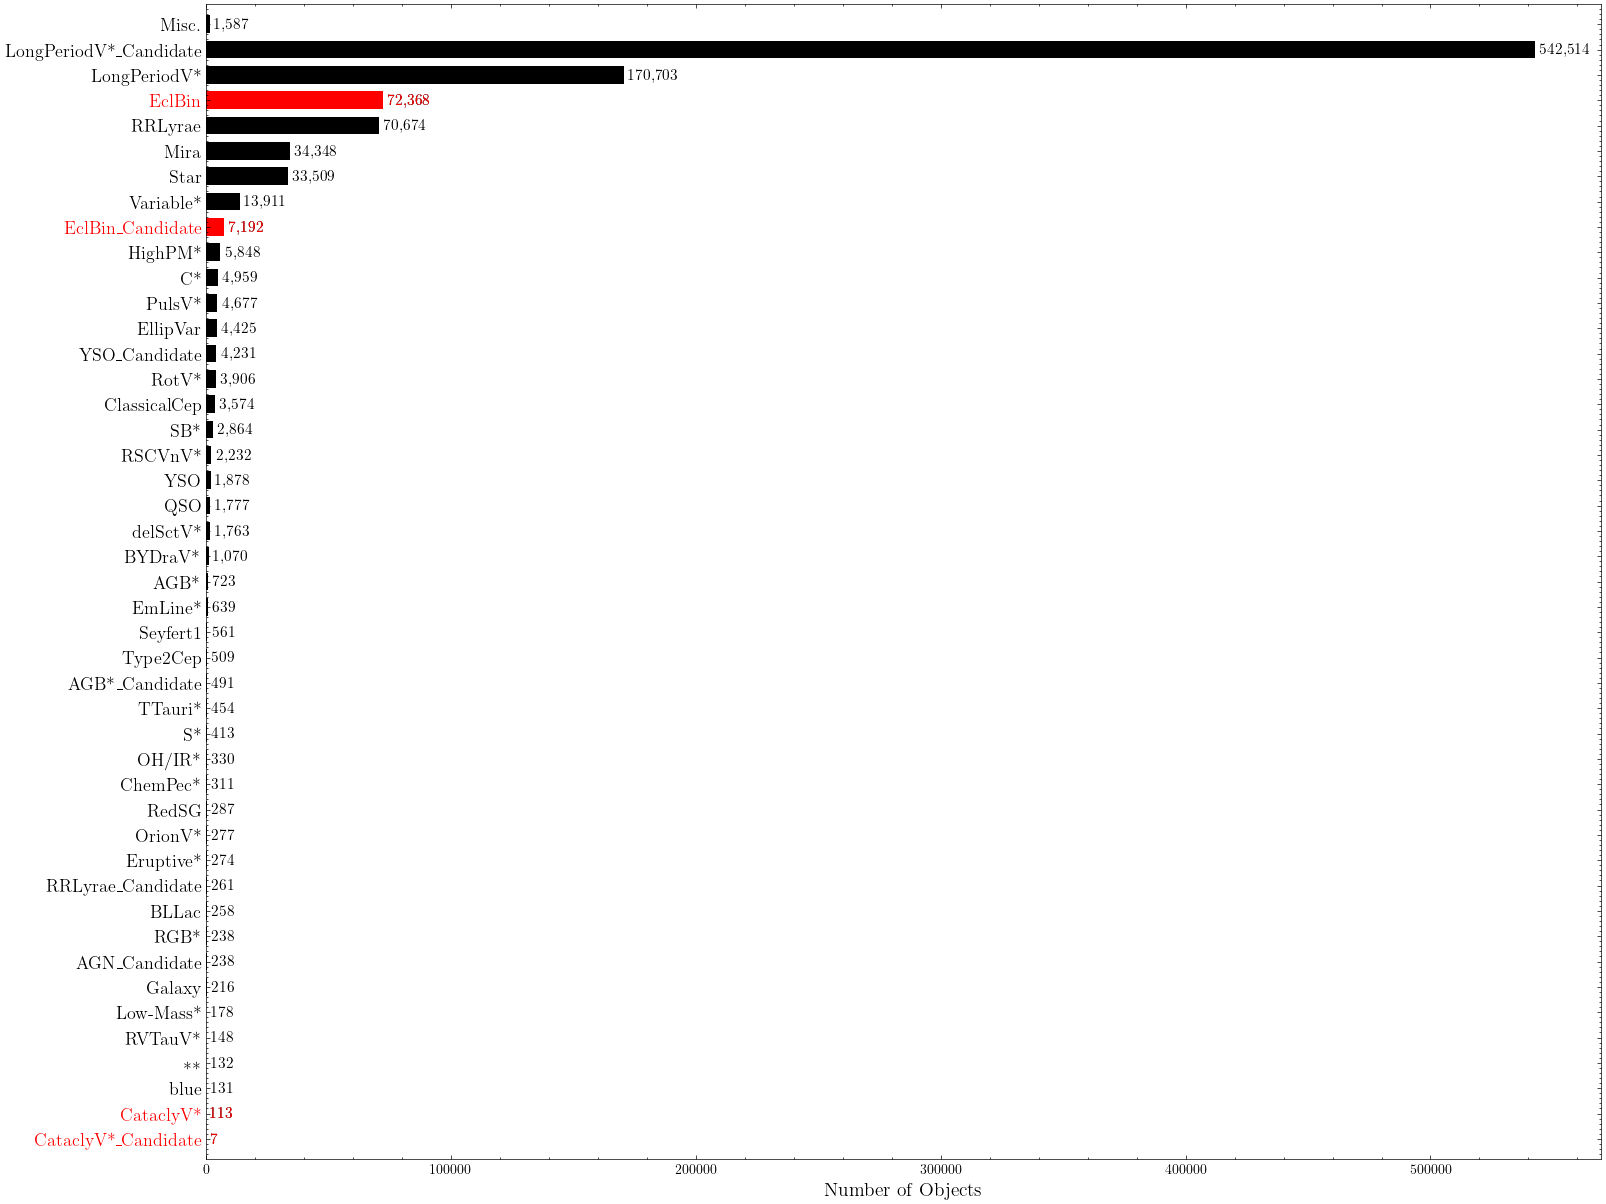
\includegraphics[scale=0.32]{Muestra/Secciones/Figures/Figura Gaia SIMBAD Busqueda Resultados.png}
	\caption{Histograma de las clasificaciones de los objetos capturados en la
	búsqueda dentro del catálogo GDR3, haciendo un análisis cruzado con la base
	de datos de SIMBAD. En rojo se resaltan las categorías de principal interés:
	los sistemas \textit{binarias eclipsantes} (\code{EclBin}) junto a las
	\textit{candidatas a binarias eclipsantes} (\code{EclBin\_Candidate}), e
	incluyendo sistemas de tipo \textit{variable cataclísmica} (\code{CataclyV*}
	y las candidatas \code{CataclyV*\_Candidate}), un tipo en particular de
	sistemas binarios en semi contacto
	(\citeyearparen{smith_cataclysmic_variables_review_2007}). Varias
	clasificaciones de baja importancia quedan agrupadas en la categoría
	\code{Misc.} por brevedad.}
	\label{figuraBusquedaSimbadHistograma}
\end{figure}

\section{ATO J339.9469+45.1464 - EclBin}

\citeyearparen{atlasATOObjectDiscovery} realizaron una búsqueda de estrellas
variables dentro de la primera publicación de datos del catálogo
\textbf{Asteroid Terrestrial-impact Last Alert System} (\textbf{ATLAS}), el cual
contiene las observaciones realizadas por el telescopio Haleakalā durante los
primeros 2 años de operación hasta finales de Junio del 2017, aprovechando su
cobertura de aproximadamente \num{13000} $\mathrm{deg}^2$ al menos 4 veces por
noche. Esta cadencia de observación es ideal para observar estrellas variables;
el tiempo de observación es suficientemente corto para obtener una curva de luz
adecuada para estudiar estos sistemas. Lograron clasificar las estrellas
variable del catálogo en 15 distintas categorías dependiendo de la morfología de
sus curvas de luz; de estas reportan que \num{74700} fuentes son binarias
eclipsantes. A pesar de haber confirmado la clasificación de estas fuentes, aún
quedan varios sistemas cuya naturaleza es desconocida.

\textbf{\atoObjIdNoSpace} está clasificado como una de estas candidatas a binaria
eclipsante. Como este sistema carece una clasificación concreta, no existe mucha
información acerca de ella. Tiene una magnitud promedio de aproximadamente
\num{16.91}, lo cual lo hace un sistema tenue. Con una ascensión recta de
\code{22 39 47.2569} y declinación de \code{+45 08 47.0311}, \atoObjId
es un sistema ideal para observar desde el OAU en Iturbide.

Antes de terminar este trabajo de maestría pero después de haber seleccionado al
objeto \atoObjId para estudiar, su clasificación en SIMBAD cambió a ser una
binaria eclipsante confirmada.
\citeyearparen{chen_ztf_catalog_periodic_variable_stars_2020} utilizaron los
datos dentro del Data Release 2 del catálogo de ZTF para clasificar varios tipos
de estrellas variables utilizando una metodología para identificar y clasificar
objetos hasta una magnitud de 20.6. Sin embargo, este estudio solo llegó a
clasificar el sistema; este trabajo de tesis profundiza el estudio para este
sistema, llegando a una solución fotométrica para determinar los parámetros
físicos del sistema.

\subsection{Datos de Gaia}

Gaia ha observado a \atoObjId durante 3 años de su operación, obteniendo
magnitudes del sistema en varias etapas en su fase empezando desde agosto del
2014 hasta mayo del 2017. En la \reffigure{gdr3AtoObjLightCurves} se pueden ver
las 3 curvas de luz de Gaia en cada pasabanda, $G_{\mathrm{BP}}$,
$G_{\mathrm{RP}}$ y $G$. Estas mediciones en distintos filtros permite el
análisis del color del sistema, el cual permite ajustar la temperatura efectiva
de una solución fotométrica a los datos observados. Este método de determinar
las temperaturas efectivas del sistema no solo nos libra de tener que utilizar
una relación empírica para darle como dato de entrada al modelo\textemdash un
ajuste de mínimos cuadrados tendrá que tomar en cuenta la física de radiación de
ambas componentes durante cualquier proceso de optimización de
parámetros\textemdash pero también permite determinar la incertidumbre de este
parámetro por medio del muestreo del espacio de parámetros libres.

% TODO: maybe move to appendix?
\begin{figure}[!ht]
	\centering
	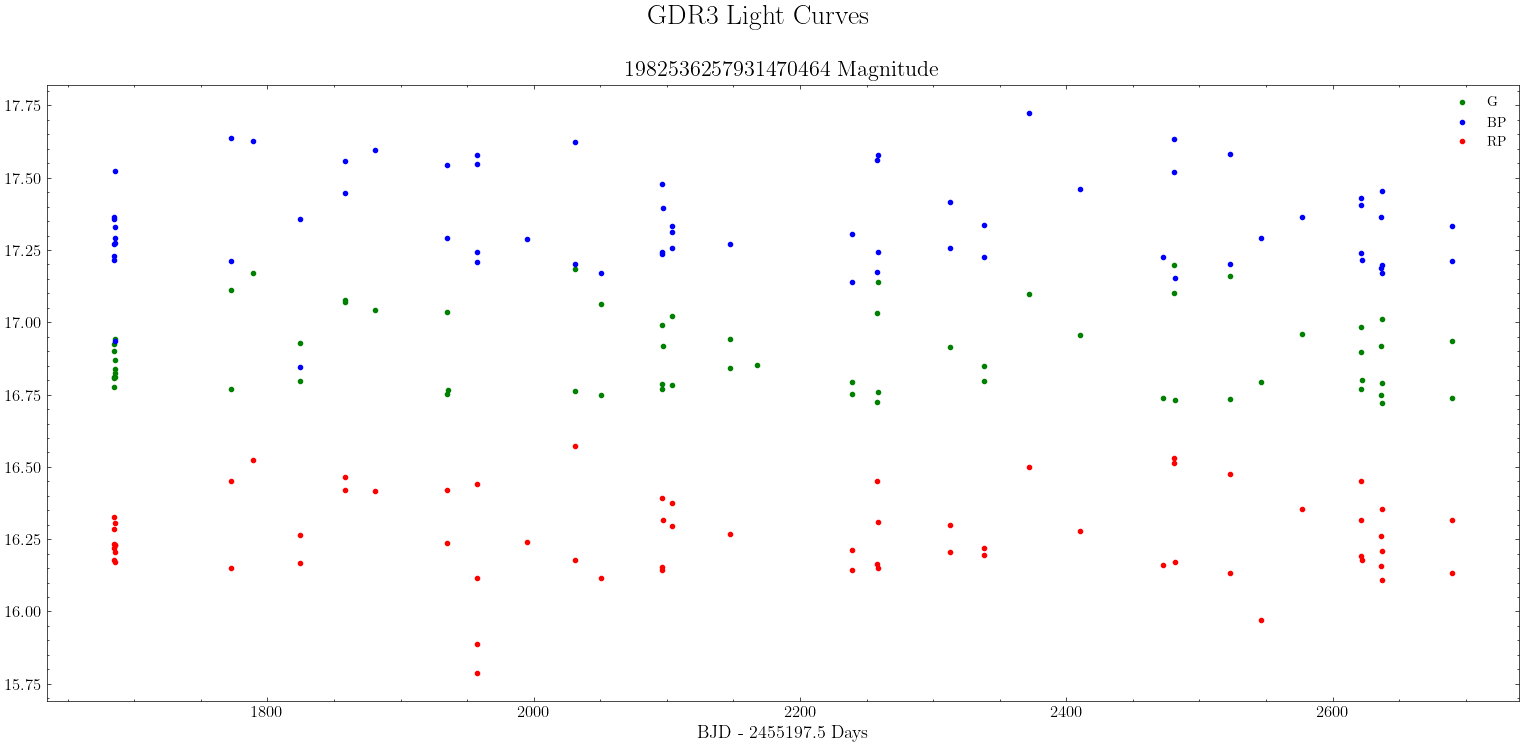
\includegraphics[scale=0.38]{Muestra/Secciones/Figures/GDR3-Light-Curves.png}
	\caption{Magnitud de \atoObjId registrada en la base de datos de Gaia DR3
	bajo su número identificador en el catálogo. La variabilidad de
	aproximadamente 0.5 mag en el brillo del sistema se atribuye a la presencia
	de eclipses en el sistema binario. Las tres curvas de luz corresponden a
	cada pasabanda de la misión de Gaia: verde es la banda $G$, en azul la banda
	$G_{BP}$, y en rojo la banda $G_{RP}$.
	(\citeyearparen{gdr3ReleaseDocumentation})}
	\label{gdr3AtoObjLightCurves}
\end{figure}

\subsection{Datos de ZTF}

Las curvas de luz de Gaia DR3 ofrecen mediciones con una precisión nunca antes
vistas. Sin embargo, el enfoque de la misión es en el cálculo de las propiedades
astrométricas de los objetos observados (incluyendo posiciones angulares,
velocidades propias, etc.); el producto principal de la misión no son las curvas
de luz fotométricas. La cadencia de observación resulta en una resolución
temporal pobre del sistema. Una dificultad adicional en el análisis de PHOEBE es
el trato de la extinción interestelar, ya que por cuestiones técnicas PHOEBE no
puede generar un modelo sintético para ciertas pasabandas cuando se aplica el
efecto de extinción interestelar; por ejemplo, PHOEBE puede calcular un
modelo que cuenta con curvas de luz en los 3 pasabandas de Gaia, pero no puede
generar una curva sintética para un modelo en las pasabandas de ZTF. Las tablas
de atmósferas estelares que PHOEBE utiliza no tienen la información necesaria
para extinguir de manera adecuada la radiación emergente para cada pasabanda.
En el caso de las curvas de luz de GDR3 esto llega a ser un problema
significativo cuando se tiene un coeficiente de extinción $E(B - V)$ apreciable,
debido a que afecta principalmente a cortas longitudes de onda.

Para complementar la información de color obtenida de Gaia y obtener una curva
de luz con alta resolución temporal\textemdash y una alta cobertura de la curva
de luz en fase\textemdash se realizó una búsqueda de datos en el catálogo de
ZTF, en particular el \textit{Data Release 20} la última versión de los datos
publicados durante la fase de recolección de datos del proyecto. Para \atoObjId
se obtuvieron 2 curvas de luz en las bandas ZTF:g y ZTF:r, las cuales no han
sido corregidas para tomar en cuenta el color del sistema en el procesamiento
hecho por IRSA. Las observaciones de ZTF se registraron desde el 20 de abril del
2018 hasta el 2 de julio del 2023 para el filtro ZTF:g, y desde el 17 de mayo
del 2018 hasta el 2 de julio del 2023 para el filtro ZTF:r. Las curvas de luz
completas se pueden ver en la \reffigure{figuraZtfCurvasLuz}.

% TODO: maybe move to appendix?
\begin{figure}[!ht]
	\centering
	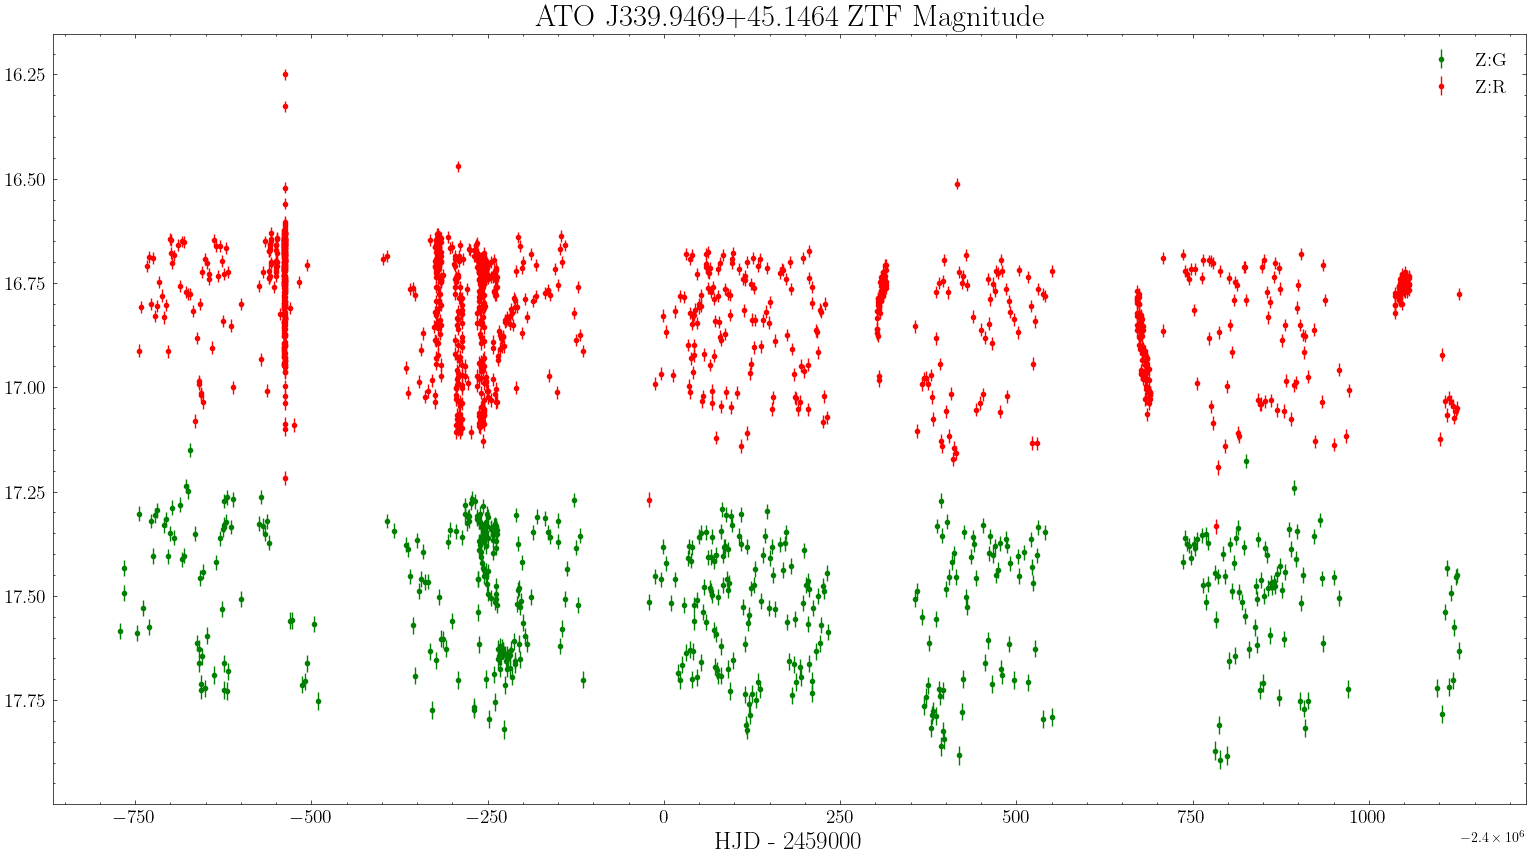
\includegraphics[scale=0.38]{Muestra/Secciones/Figures/Figura ZTF Light Curves.png}
	\caption{Curvas de luz en las pasabandas ZTF:g (verde) y ZTF:r (rojo) para \atoObjId, 
	obtenido del catálogo de ZTF por su identificador de SIMBAD.}
	\label{figuraZtfCurvasLuz}
\end{figure}
\chapter{Observaciones}

El segundo objetivo principal de este trabajo de tesis de maestría es realizar
una campaña de observación a \atoObjId. Desde el \textbf{Observatorio
Astronómico Universitario} en Iturbide, N.L. se midió el brillo del sistema
durante 9 noches de observación; mediante la técnica de fotometría diferencial
se obtiene una curva de luz, la cual se utiliza para determinar la naturaleza
del objeto observado.

\section{Observatorio Astronómico Universitario - Iturbide}

El \textbf{Observatorio Astronómico Universitario - Iturbide} (el cual de ahora
en adelante será referido como el OAU), ubicado en el cerro Picacho en el
municipio de Iturbide, Nuevo León, es un nuevo sitio dedicado a la observación
astronómica, equipado para realizar observaciones del Sol, monitoreo de basura
espacial, y la observación de objetos variables, como los sistemas binarios o
asteroides. A continuación se describe el equipo utilizado; como software de
control se utilizó \textbf{Nighttime Imaging 'N'
Astronomy}\footnote{\myurl{https://nighttime-imaging.eu}} (\textbf{NINA}), el cual
permita consolidar el control de todas las componentes mecánicas en una sola
aplicación. 

% TODO: look for mount documentation
El telescopio utilizado para hacer las observaciones del sistema fue el tubo
óptico \textbf{CDK20} de \textbf{PlaneWave
Instruments}\footnote{\myurl{https://planewave.com/product/cdk20-ota/}} con un
número $f/6.8$. Este telescopio de diseño \textit{Dall-Kirkham corregido} cuenta
con un grupo de lentes frente al espejo esférico secundario, el cual resta los
efectos de la aberración esférica presente en otras configuraciones de espejos
primarios y secundarios, resultando en una imagen más nítida. Este instrumento,
combinado con una montura ecuatorial \textbf{Orion HDX110}, nos permite una
vista clara de la bóveda celeste a \ang{30} arriba del horizonte, con capacidad
de observar objetos tenues más allá de 17 magnitudes.

El CCD usado para obtener las imágenes fue el
\textbf{QHY174GPS}\footnote{\myurl{https://www.qhyccd.com/qhy174gps-imx174-scientific-cooled-camera/}}.
Este CCD cuenta con una resolución de $1920 \times 1200$ pixeles. Para reducir
el ruido térmico tiene un mecanismo de enfriamiento termoeléctrico, el cual lo
puede enfriar a una temperatura de -\ang{40} C bajo la temperatura ambiente.
Frente al CCD va equipado una rueda de filtros \textbf{ZWO
7x36mm}\footnote{\myurl{https://astronomy-imaging-camera.com/product/new-zwo-efw-7x36mm/}},
la cual puede ser equipada con 7 filtros distintos. Para las observaciones
recabadas en este trabajo, utilizamos solamente el filtro \textbf{Luminance}, el
cual se aproxima a la región del visible del espectro electromagnético
(\reffigure{zwoFilterTransmissionCurve}). 

\begin{figure}[!ht]
	\centering
	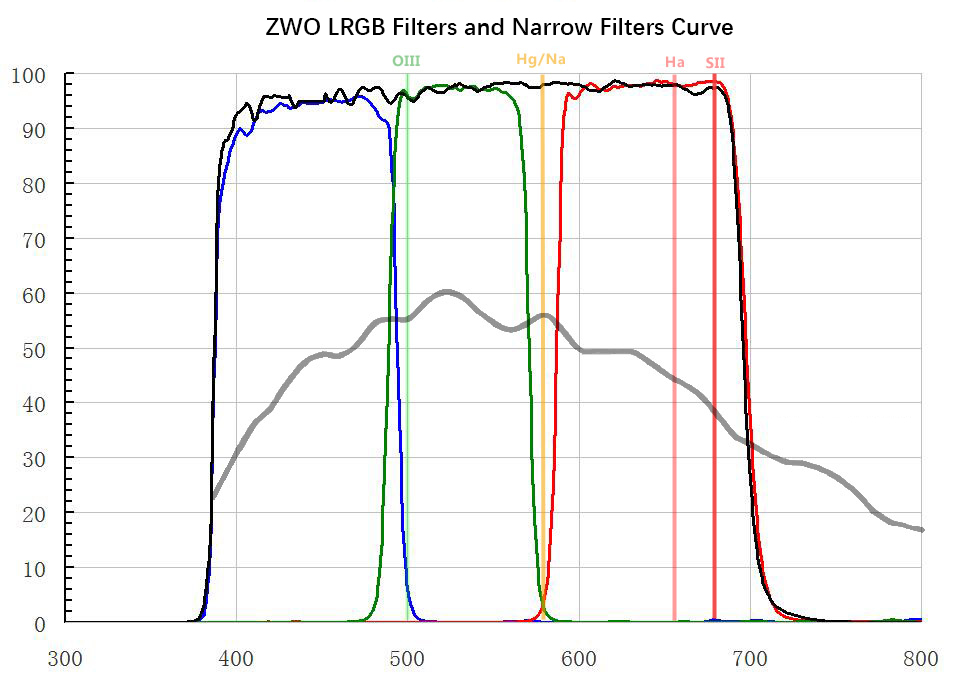
\includegraphics[scale=0.6]{Observaciones/Secciones/Figures/ZWO RGBL Transmission Curve.jpg}
	\caption{Curva de transmisión de filtros de ZWO. El filtro de
	\textbf{Luminance} se encuentra como la curva negra, abarcando todo el
	espectro visible, desde los 400nm hasta 700nm. Gráfica obtenida de la
	\href{https://astronomy-imaging-camera.com/product/zwo-lrgb-36mm-filters/}{página
	de productos de ZWO}.}
	\label{zwoFilterTransmissionCurve}
\end{figure}
\section{Fotometría}

Para este trabajo se realizó una campaña de observación durante los últimos
meses del 2022, con la finalidad de observar el sistema durante una fase orbital
completa. Las fechas y duraciones de cada día de observación se encuentra en la
\reftable{observationSchedules}. Varias de las noches de observaciones sufrieron
de pobres condiciones del sitio, las cuales llegaron a afectar la calidad de las
observaciones; tanto las condiciones meteorológicas como contratiempos causados
por el equipo en si causaron interrupciones en las exposiciones continuas y
perturbaciones en las imágenes mayores a las que se puede corregir en el
procesamiento de datos. Esto es esperado en un observatorio en proceso de
desarrollo; a pesar de los problemas técnicos, se pudieron obtener datos de
calidad aceptable. Los vientos fuertes fueron un gran obstáculo debido a la nula
protección del CCD montado al telescopio, ya que cualquier perturbación por
parte del viento resultaba en una imagen defectuosa. Dado que las observaciones
de este proyecto se realizaron en el 2022 solo el viento sigue siendo un
problema para observaciones posteriores; todavía no se implementa una cúpula
para proteger el telescopio del viento, pero el auto-enfocador y guiador están
funcionando de manera apropiada.

% TODO: style table
\begin{table}[!ht]
	\centering
	\begin{tabular}{|c|c|c|c|}
		\hline
		\thead{Fecha (UTC)} & \thead{HJD Inicio +\textbf{\num{2459000}}} & \thead{Tiempo Expocisiones} & \thead{Duración} \\
		\hline
		2022-10-22 & 874.67 & $111 \cdot 60$ s & 2.67 h \\
		\hline
		2022-10-23 & 875.57 & $159 \cdot 60$ s & 5.28 h \\
		\hline
		2022-10-28 & 880.77 & $124 \cdot 60$ s & 2.11 h \\
		\hline
		2022-11-06 & 889.58 & $125 \cdot 60$ s & 4.25 h \\
		% \hline
		% 2022-11-26 & 910.72 & $56 \cdot 60$ s & 1.55 h \\
		\hline
		2022-12-07 & 920.55 & $231 \cdot 60$ s & 5.25 h \\
		\hline
		2022-12-08 & 921.57 & $138 \cdot 60$ s & 4.25 h \\
		\hline
		2022-12-09 & 922.54 & $127 \cdot 60$ s & 4.97 h \\
		\hline
		2022-12-10 & 923.54 & $129 \cdot 60$ s & 5.44 h \\
		\hline
		2022-12-11 & 924.53 & $122 \cdot 60$ s & 2.20 h \\
		\hline

	\end{tabular}
	\caption{Bitácora de fechas de observaciones fotométricas desde el OAU.}
	\label{observationSchedules}
\end{table}

\subsection{Estrellas de Comparación}

Para determinar la magnitud diferencial de un objeto se necesita una estrella de
comparación dentro del campo de la imagen de ciencias. Una manera de
encontrar estrellas de referencias adecuadas es utilizando el Variable Star
Plotter\footnote{\url{https://app.aavso.org/vsp/}} de la \textit{AAVSO}; sin
embargo, debido al pequeño campo de visión de nuestras imágenes
(aproximadamente $1^{\prime}$ de largo), no se encuentra alguna estrella
standard registrada. Por lo tanto para realizar la fotometría diferencial solo
es necesario tener estrellas de comparación con un número de cuentas (flujo
integrado) similar al objeto de interés. El campo visible de \atoObjId
utilizando el equipo de OAU se puede ver en la \reffigure{figuraCcdCampo}.

\begin{figure}[!ht]
	\centering
	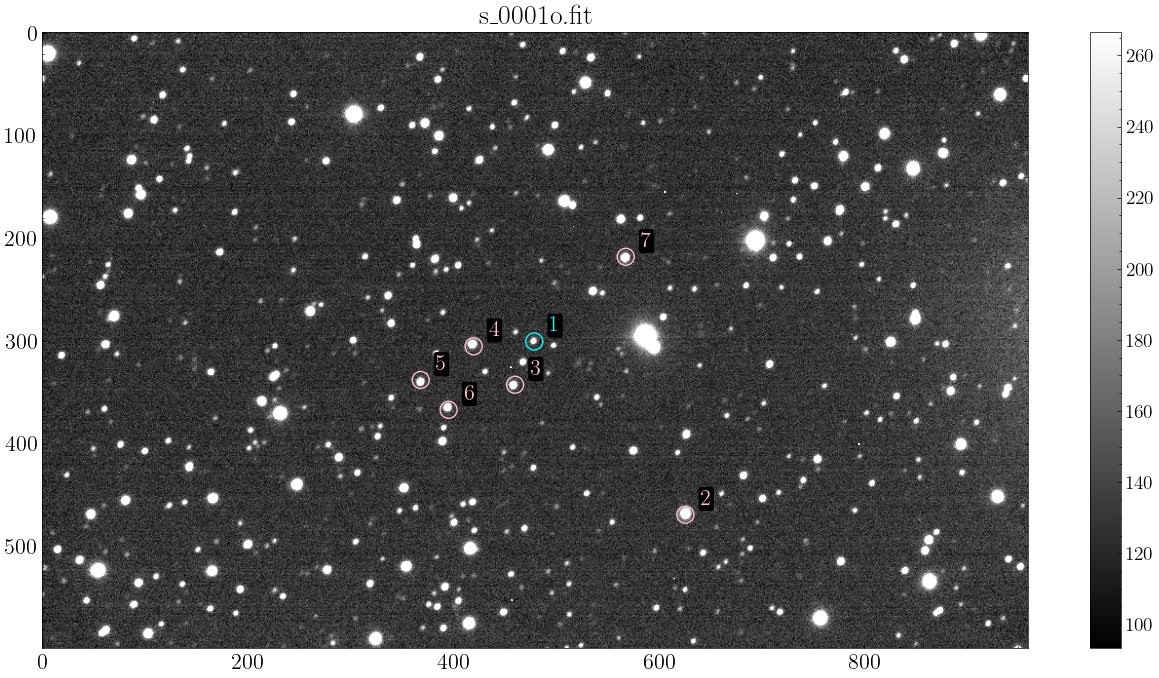
\includegraphics[scale=0.5]{Observaciones/Secciones/Figures/Figura Campo Observado.png}
	\caption{Imagen del campo de \atoObjId marcado con la etiqueta $1$ en, 
	junto a las estrellas de referencia usadas en la fotometría diferencial 
	marcadas en anillos rosas marcados con etiquetas del $2$ al $7$.}
	\label{figuraCcdCampo}
\end{figure}

\subsection{Procesamiento de Imágenes}

La limpieza de las imágenes incluyó la corrección de bias, darks, y flats por
medio de imágenes de calibración, las cuales fueron tomadas cada noche de
observación. Esto fue realizado utilizando tareas standard de IRAF
(\citeyearparen{tody_iraf_1986}). Cada imagen fue revisada manualmente para
determinar si era de suficiente calidad para hacer una medición adecuada. Se
analizó la forma que proyecta el objeto en la imagen del CCD; solo las imágenes
cuyo perfil se aproxima a un circulo fueron aceptadas para realizar el proceso
de fotometría diferencial.

\begin{figure}[!ht]
	\centering
	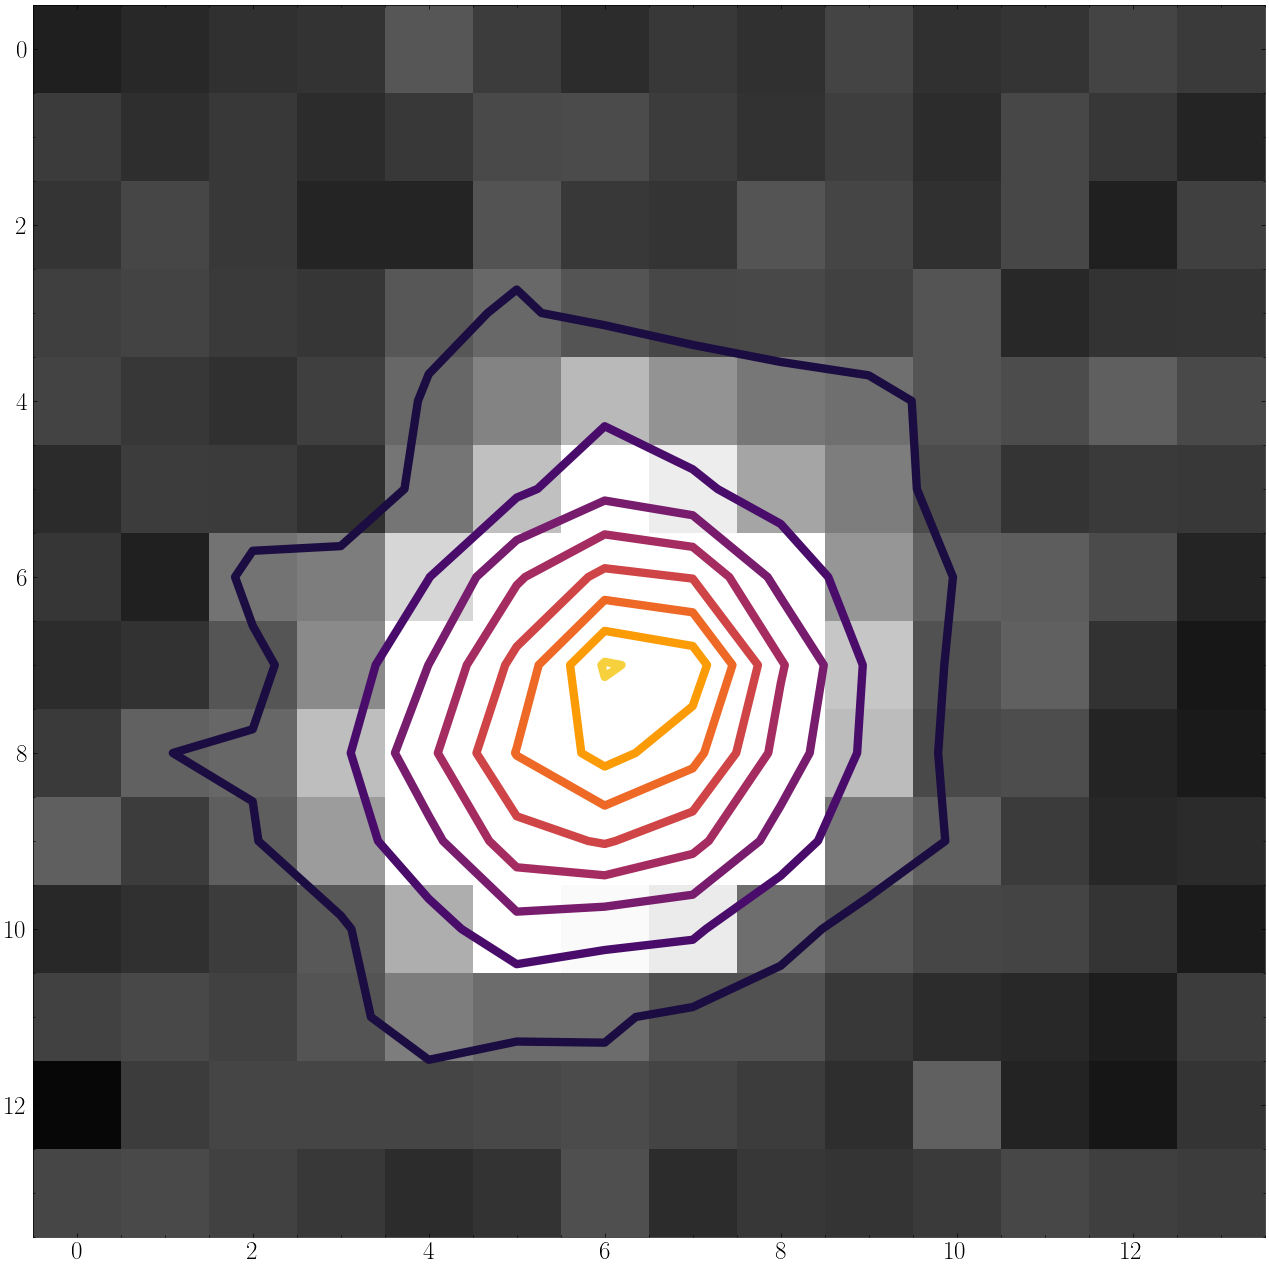
\includegraphics[scale=0.4]{Observaciones/Secciones/Figures/Figura Pixel Perfil Contorno.png}
	\caption{Isógrama de las cuentas registradas del flujo de \atoObjId para un
	corte de $14 \times 14$ pixeles, donde el color más claro denota una mayor
	cantidad de cuentas.}
	\label{figuraPixelContorno}
\end{figure}

Una vez que las mediciones fueran corregidas, fue necesario trasladar los datos
dentro de las imágenes para que \atoObjId quede en el centro del campo,
facilitando la fotometría por apertura. Utilizando el script
\href{https://github.com/KnightIV/UANL_MAPTA_Observaciones/blob/main/analisis/iturbide/shift_images.py}{\code{shift\_images.py}}
se ejecutó una tarea de \textit{plate solving} para cada imagen calibrada; el
proceso de \textit{plate solve}, llevado a cabo utilizando el programa
\textit{Astrometry} (\citeyearparen{astrometry}), toma como referencia estrellas
dentro del campo de la imagen comparando contra una base de datos pre-definida
para determinar las coordenadas físicas que corresponden a una imagen. Esta
información va encapsulada dentro de los metadatos del archivo FITS, conocido
como \textbf{World Coordinate System} (\textbf{WCS}). Una vez que una imagen sea
resuelta se puede proyectar a las coordenadas de otra imagen, posicionando la
estrella variable en una posición única dentro del encuadro de cada imagen,
facilitando el uso de coordenadas en pixeles para definir las aperturas de
medición fotométrica.

Utilizando las imágenes proyectadas se obtuvo el brillo del objeto utilizando
la tarea \code{qphot} de IRAF, dando como resultado magnitudes instrumentales
del sistema. La apertura en tamaño de pixeles se definió en base al ancho a
media altura (\textit{full-width at half-maximum}) de \atoObjId para cada
imagen, utilizando la tarea \code{imexam} de IRAF. Este se usó como el radio de
la apertura circular, junto a una apertura anular para sustraer el brillo de
fondo del cielo, el cual se utilizó para las 7 estrellas marcadas en la
\reffigure{figuraCcdCampo}. Las magnitudes instrumentales medidas se pueden ver
en la \reffigure{figuraCurvaLuzInstrumentalTodas}. A pesar de que todos los
objetos muestran un comportamiento variable, esto no es una característica
intrínseca de todos los sistemas. En particular, la estrella de comparación se
considera que emite un flujo relativamente constante a comparación del sistema
variable \atoObjIdNoSpace; por lo tanto, las variaciones vistas en su curva de
luz se deben a perturbaciones atmosféricas e instrumentales, lo cual nos permite
eliminar estos efectos por medio de la fotometría diferencial.

\begin{figure}[!ht]
	\centering
	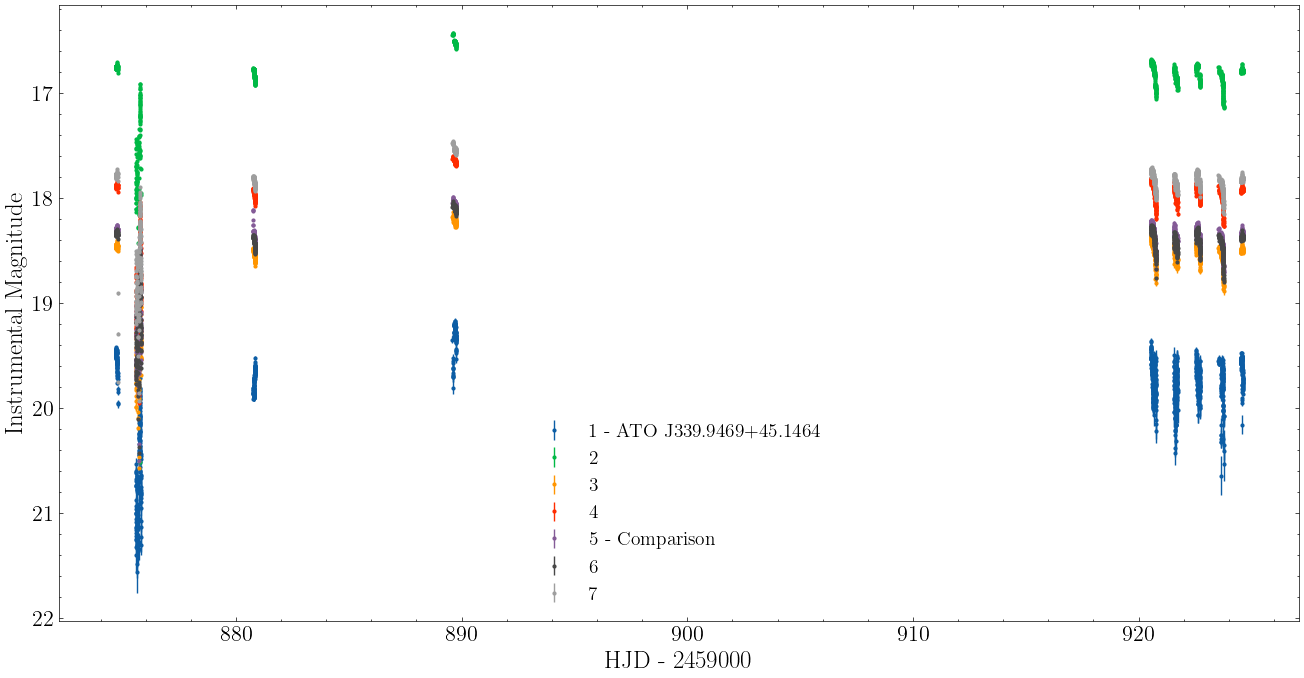
\includegraphics[scale=0.4]{Observaciones/Secciones/Figures/Figura Magnitud Instrumental Todas.png}
	\caption{Magnitudes instrumentales reportada por IRAF mediante la técnica de
	fotometría de apertura. De los 7 objetos resaltados en la
	\reffigure{figuraCcdCampo} se distinguen el objeto principal \atoObjId con
	la etiqueta $1$, y la estrella de referencia utilizada para determinar la
	magnitud diferencial de \atoObjIdNoSpace. }
	\label{figuraCurvaLuzInstrumentalTodas}
\end{figure}

\subsection{Fotometría Diferencial}
Para obtener una magnitud diferencial de \atoObjId se necesita de una estrella
de referencia de la cual se observe un flujo constante. Aparte del requisito de
ser una fuente constante, una estrella de referencia ideal sería del mismo color
que el sistema variable \atoObjIdNoSpace; sin embargo, en casos como el de este
estudio se puede despreciar este último requisito debido al bajo número de
opciones disponibles dentro del campo visible. Del campo visible en la
\reffigure{figuraCcdCampo} se eligió el objeto número $5$ como la estrella de
referencia. Su curva de luz instrumental se puede ver a mayor detalle en la
\reffigure{figuraCurvaLuzInstrumentalReferencia}. La magnitud diferencial $m_d$
de \atoObjId se obtiene restando la magnitud instrumental del objeto de
referencia 5 $m_{\mathrm{inst, 5}}$ de la magnitud instrumental medido de
\atoObjId $m_{\mathrm{inst, \atoObjId}}$ utilizando la
\refequation{ecuacionMagnitudDiferencial}, cuya curva de luz resultante se puede
ver en la \reffigure{figuraIturbideAtoLightCurve}. Las imágenes calibradas se
encuentran como un \textit{Release} dentro del repositorio de GitHub este
proyecto de investigación, junto a los datos de la fotometría de
apertura.\footnote{\url{https://github.com/KnightIV/UANL_MAPTA_Observaciones/releases/tag/data}}

\begin{eqfloat}[!ht]
	\begin{equation}
		m_d = m_{\mathrm{inst, \atoObjId}} - m_{\mathrm{inst, 5}}
	\end{equation}
	\blankcaption
	\vspace{-0.5em}
	\label{ecuacionMagnitudDiferencial}
\end{eqfloat}

\begin{figure}[!ht]
	\centering
	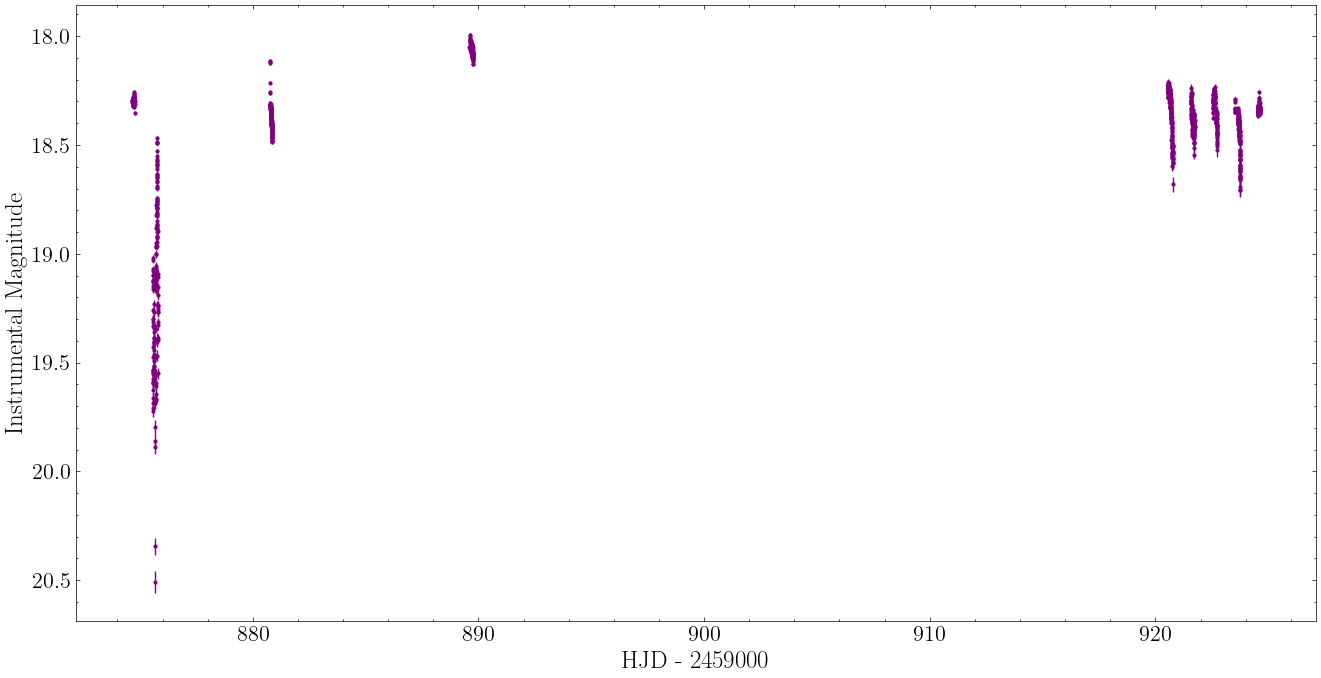
\includegraphics[scale=0.44]{Observaciones/Secciones/Figures/Figura Magnitud Instrumental Estrella Referencia.png}
	\caption{Magnitud instrumental de la estrella de referencia utilizada para
	determinar la magnitud diferencial de \atoObjIdNoSpace. La variabilidad en
	la curva de luz se atribuye a factores extrínsecos del sistema.}
	\label{figuraCurvaLuzInstrumentalReferencia}
\end{figure}

\begin{figure}[!ht]
	\centering
	\xincludegraphics[scale=0.42, label=\textbf{(a)}, labelbox=true, pos=nw, fontsize=\large]{Observaciones/Secciones/Figures/Full LC.png}
	\xincludegraphics[scale=0.34, label=\textbf{(b)}, labelbox=true, pos=nw, fontsize=\large]{Observaciones/Secciones/Figures/Hour Sync LC.png}
	\caption{Magnitud diferencial de \atoObjIdNoSpace. \textbf{(a)} Curva de luz
	completa. \textbf{(b)} Curva de luz segmentada por día, con la cual se logra
	apreciar la cadencia de observación, viendo como cada día se logra observar
	una fase diferente del sistema.}
	\label{figuraIturbideAtoLightCurve}
\end{figure}
\part{Metodología y Análisis de Datos}

% TODO: make abstract

\chapter{Periodo Orbital} \label{metodologia:analisisperiodo}

Una de las propiedades más importantes presente en la curva de luz de una
binaria eclipsante es su \textbf{periodo orbital}. Partiendo del periodo orbital
es posible presentar los datos observacionales en el espacio fase en vez de
tiempo, el cual nos permite ajustar modelos analíticos para determinar ciertas
propiedades del sistema binario. Dada una curva de luz se puede encontrar el
periodo orbital usando \textbf{periodogramas}: herramientas utilizadas para
generar un espectro de potencias para una serie de tiempo periódica. Para series
de tiempo cuyo muestreo no es uniforme en el tiempo (como es común de
observaciones astronómicas) se utiliza el periodograma \textbf{Lomb-Scargle},
derivado de la transformada de Fourier \brakcite{vanderplas_understanding_lomb_scargle_periodogram_2018}.
Usando un mallado suficientemente fino para explorar el espacio de frecuencias
se puede encontrar la frecuencia de mayor potencia, indicando el periodo orbital
del sistema; al mismo tiempo, para restringir esta malla de periodos se impuso
un límite máximo de 1 día, basado en las primeras observaciones de Iturbide. El
espectro de frecuencias se encuentra en la \reffigure{periodogramaLSFrecs}. 

\begin{figure}[!h]
	\centering
	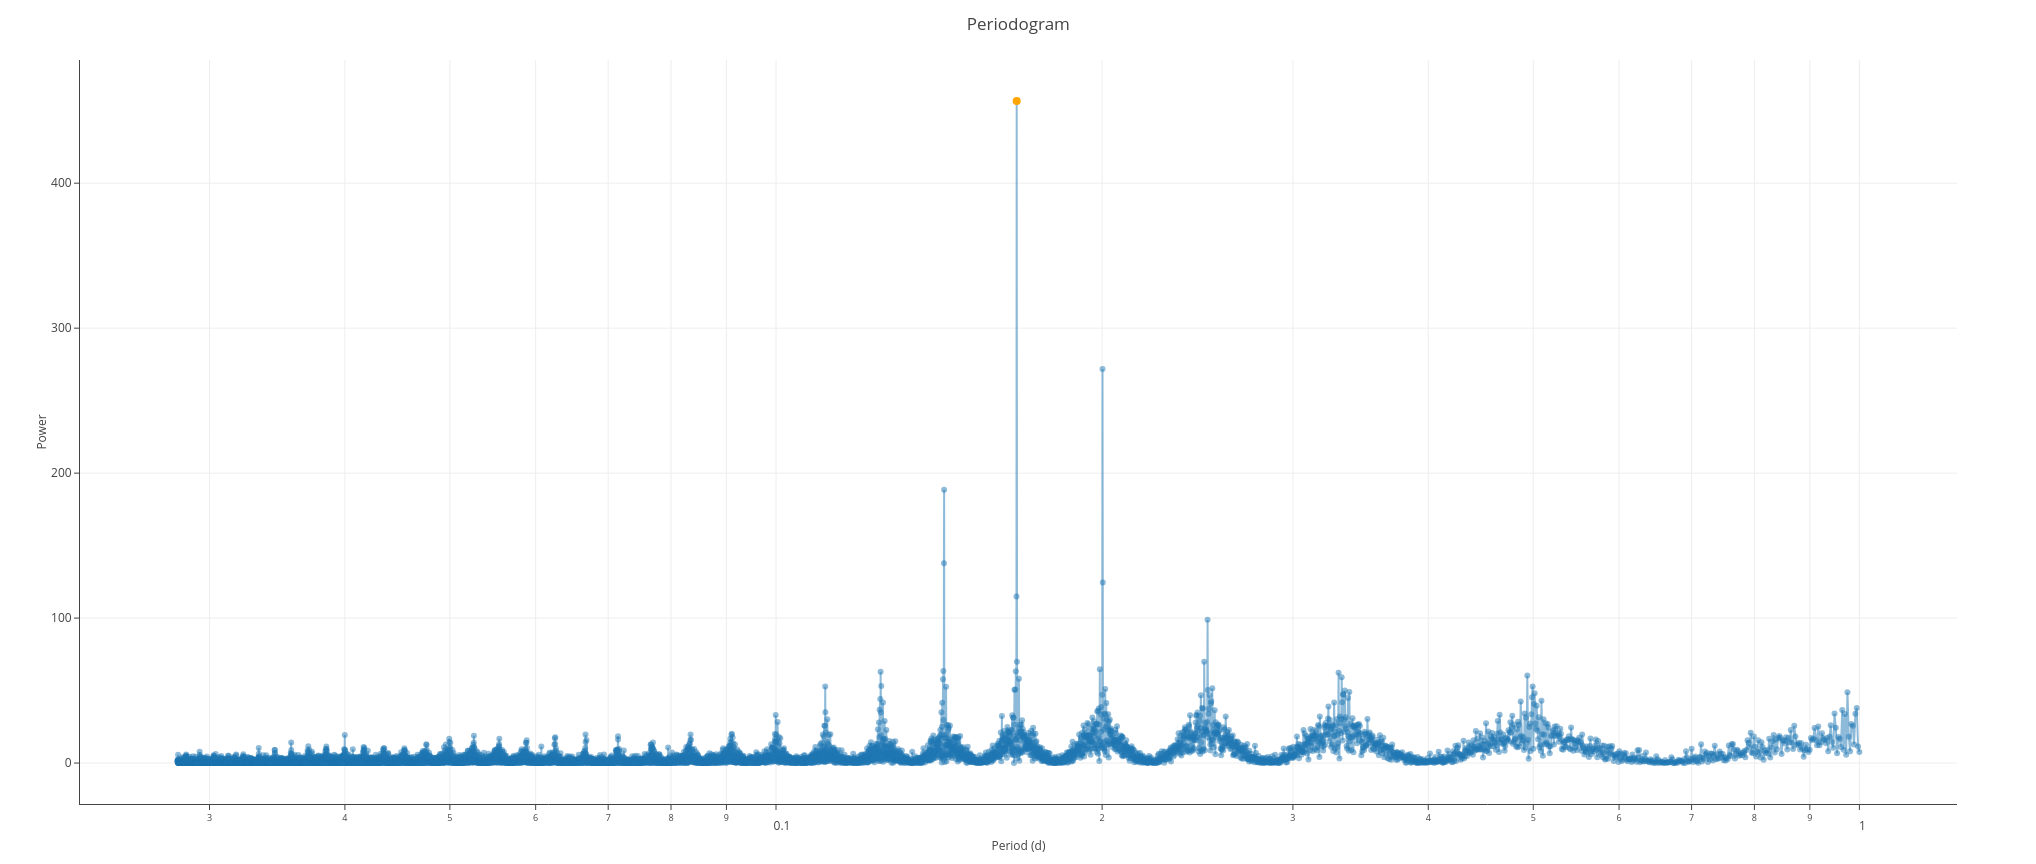
\includegraphics[scale=0.23]{Metodologia/Secciones/AnalisisPeriodo/Figures/IRSA Periodogram.png}
	
	\caption{Espectro de frecuencias de las curvas de luz fotométricas de
	\atoObjIdNoSpace, utilizando observaciones de ZTO en el filtro R. Este
	periodograma fue generado utilizando la herramienta del IRSA dedicada al
	análisis de series de tiempo, \textbf{Time Series Tool}. El pico de más alta
	potencia está ubicado en el periodo de 0.1667834993 d [4.002803983 h]} 
	\label{periodogramaLSFrecs}
\end{figure}

Dado este espectro de frecuencias encontramos que el periodo orbital yace en la
segunda armónica de la frecuencia principal. Esto se debe a los requisitos para
analizar una curva de luz de un sistema binario eclipsante; estos muestran dos
valles en el espacio fase, las cuales corresponden a las etapas en la curva de
luz en las que se observan eclipses en el sistema. Esto es necesario para poder
modelar la curva de luz en fase como una Gaussiana doble, el modelo aceptado
para una binaria eclipsante. %TODO: agrega bibliografía
Utilizando la segunda armónica de la frecuencia de más alta potencia se puede
ver esta forma esperada de la curva de luz, como se puede ver en la
\reffigure{gaiaIturbideZtfPhaseFold}. El periodo orbital encontrado es de
8.005607976 horas.

\begin{figure}[!h]
	\centering
	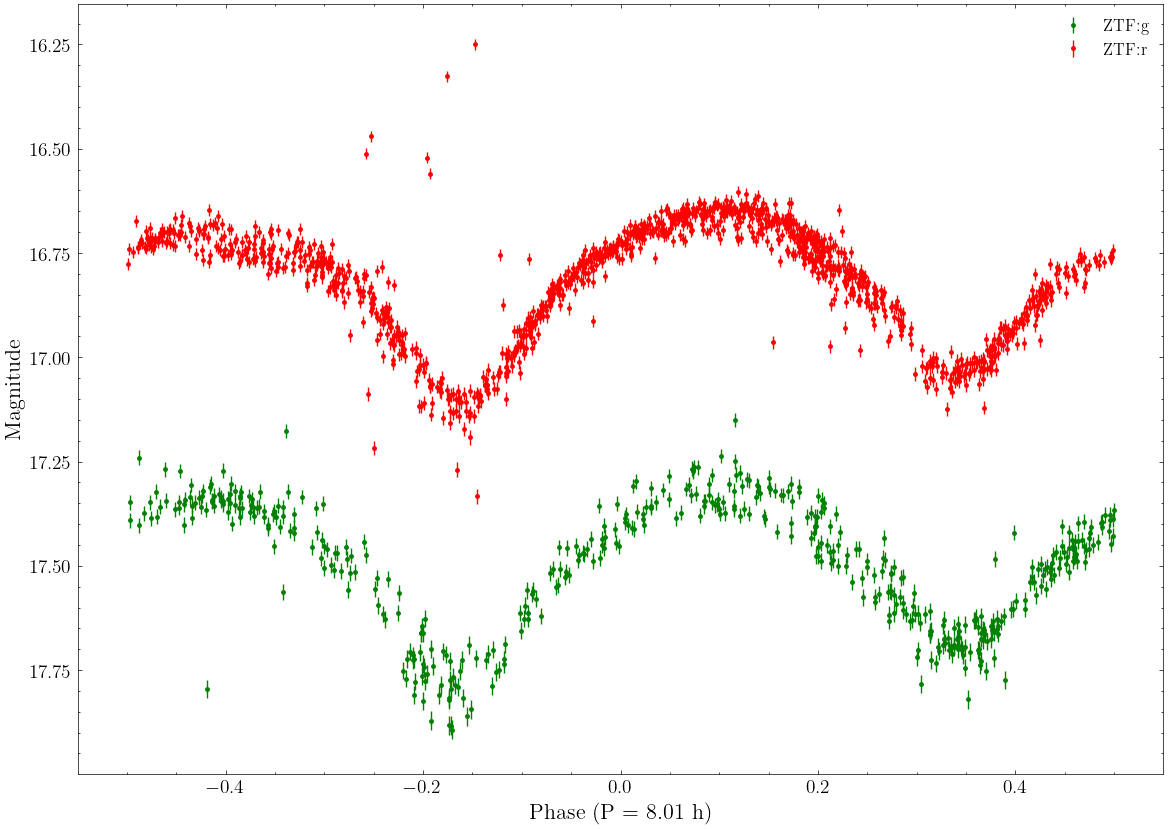
\includegraphics[scale=0.3]{Metodologia/Secciones/AnalisisPeriodo/Figures/ZTF Phase-Folded.png}
	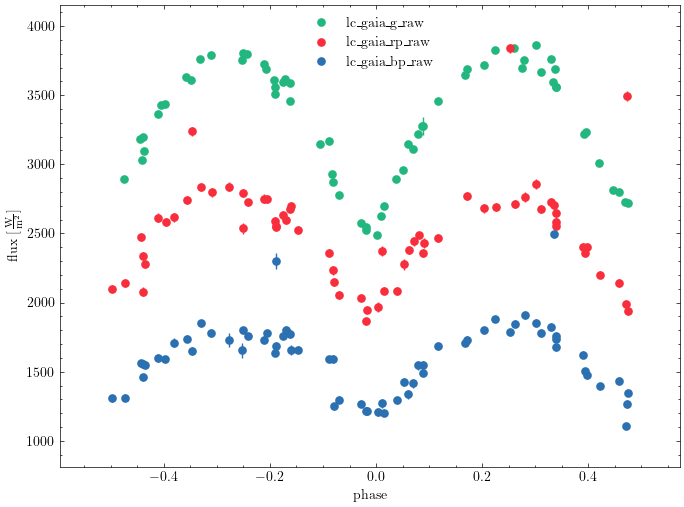
\includegraphics[scale=0.3]{Metodologia/Secciones/AnalisisPeriodo/Figures/Gaia Phase-Folded.png}
	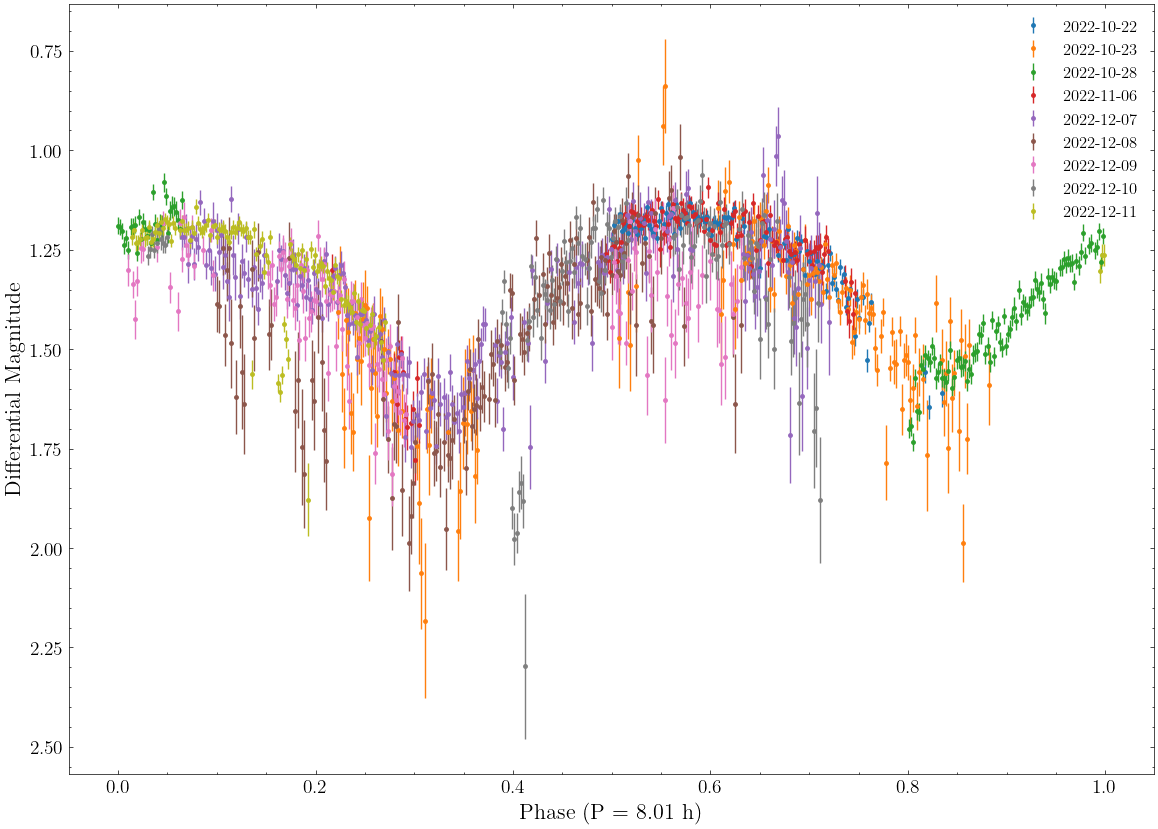
\includegraphics[scale=0.4]{Metodologia/Secciones/AnalisisPeriodo/Figures/Iturbide Phase-Folded.png}

	\caption{Curvas de luz de ZTF, Gaia e Iturbide en espacio fase dado un
		periodo orbital de 8.005607976 horas. El tiempo de conjunción superior
		son corregidos en los siguientes pasos de afinación del modelo de
		PHOEBE, el cual ajusta la fase 0 para que coincidan las 3 curvas de luz.
		Las observaciones de Iturbide se clasifican por su noche de observación,
		indicado por su color.}
	\label{gaiaIturbideZtfPhaseFold}
\end{figure}
\section{Normalización de Flujos} \label{Metodologia:NormalizacionFlujos}

Tenemos a nuestra disposición las cuentas de fotones que corresponden a sus
magnitudes para las curvas de luz de Gaia, para las cuales el flujo reportado es
el promedio de todas las mediciones hechas en un transito, e Iturbide. Sin
embargo, estas cuentas crudas no son adecuadas para el ajuste de modelo con
PHOEBE; estas producen resultados no físicos cuando son utilizadas sin
tratamiento adicional. Para esto las magnitudes determinadas en la sección
anterior se convierten a flujos normalizados con la
\refequation{normFlujosEcuacion}. Esta transformación fue aplicada a todas las
curvas de luz recabadas (Gaia, ZTF, Iturbide) para poder trabajar con datos
consistentes al momento de desarrollar el modelo computacional en PHOEBE.

\begin{eqfloat}[!ht]
	\centering
	\begin{equation}
		f_p = 10^{-\frac{2}{5} \cdot (m_p - m_0)}
	\end{equation}
	\caption{Ecuación usada para obtener flujos para cada pasa banda $p$. Esta
		determina el flujo normalizado $f_p$ desde la magnitud reportada $m_p$
		utilizando una magnitud de referencia $m_0$.}
	\label{normFlujosEcuacion}
\end{eqfloat}

\subsection{Preservación de Color}

% TODO: figure out how to cite specific chapter of PHOEBE textbook (page 111) without having to create a bunch of citations for each section used
	% ideally would mention the chapters/pages used in a single citation
Gracias a las observaciones en varias pasa bandas tenemos información del color
del sistema, debido a la diferencia de magnitud. Sin embargo PHOEBE trabaja solo
con flujos, por lo cual la transformación descrita en la
\quotesection{Metodologia:NormalizacionFlujos} fue necesaria. Para preservar el
color por diferencia de magnitud se determina un solo valor de $m_0$ con el cual
convertir las magnitudes; este $m_0$ corresponde a la magnitud en 0.25 de fase
del pasa bandas más tenue del sistema. PHOEBE tablas de coeficientes que
relacionan la temperatura efectiva del sistema binario con la diferencia de
flujos. \brakcite{phoebeScientificReference} 

En este trabajo se dividieron las curvas de luz de \atoObjId basado en su
fuente: las de Gaia ($G, G_{BP}, G_{RP}$), las de ZTF ($ZTF:G, ZTF:R$), y la de
Iturbide. Podemos determinar 2 diferentes colores del sistema, entre la
diferencia de color en Gaia y ZTF (como solo se observó a \atoObjId con un solo
filtro en Iturbide no contamos con datos de color). Para ZTF se tomó la
magnitud de $ZTF:G$. Las curvas de luz en fase se pueden ver en la
\reffigure{normFlujosCurvas}, donde se puede apreciar como preserva la
diferencia de magnitud vista en \reffigure{gaiaIturbideZtfPhaseFold}. El
código responsable de esta reducción se encuentra en
\href{https://github.com/KnightIV/UANL_MAPTA_Observaciones/blob/main/analisis/gaia/light_curves.ipynb}{\code{light\_curves.ipynb}}
para Gaia,
\href{https://github.com/KnightIV/UANL_MAPTA_Observaciones/blob/main/analisis/ztf/light-curve-processing.ipynb}{\code{light-curve-processing.ipynb}}
para ZTF, y
\href{https://github.com/KnightIV/UANL_MAPTA_Observaciones/blob/main/analisis/iturbide/iraf/qphot_timeseries_analysis.ipynb}{\code{qphot\_timeseries\_analysis.ipynb}}
para Iturbide.

\begin{figure}[!ht]
	\centering
	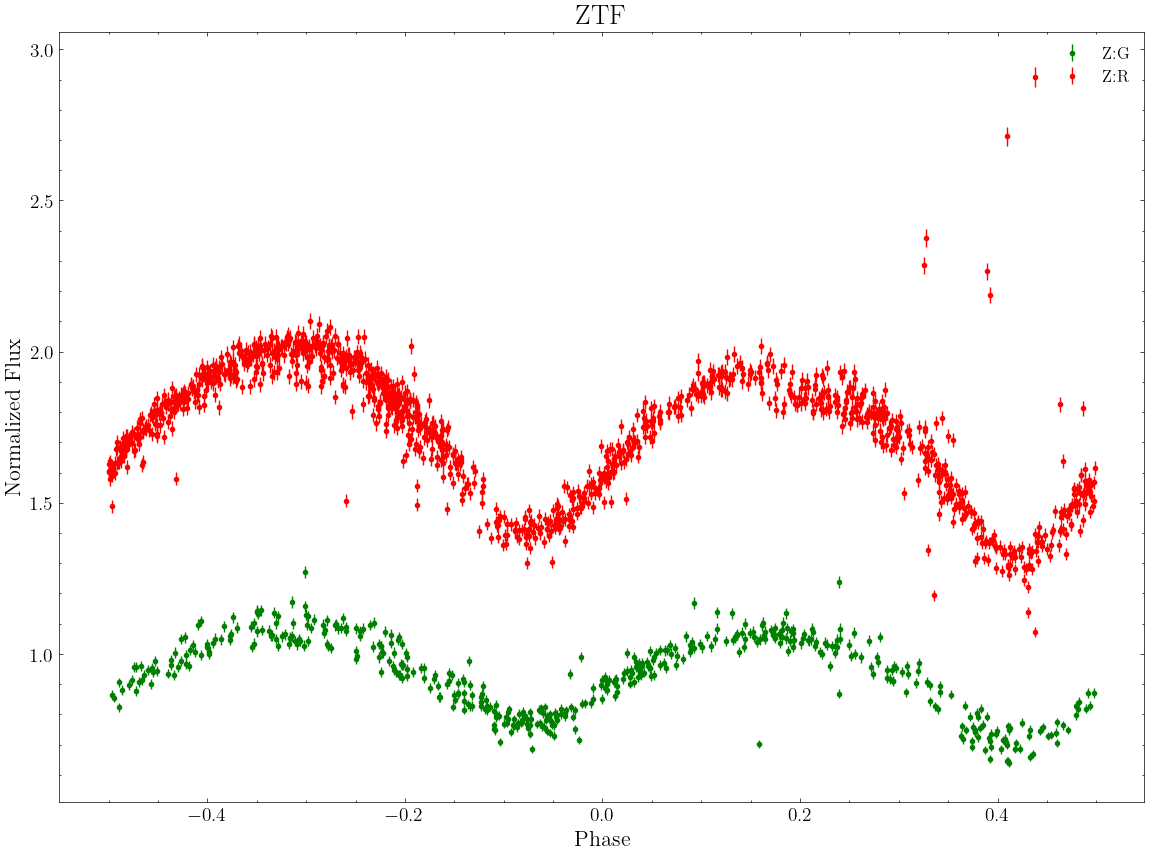
\includegraphics[scale=0.3]{Metodologia/Secciones/NormalizacionFlujos/Figures/ZTF Normalized Flux.png}
	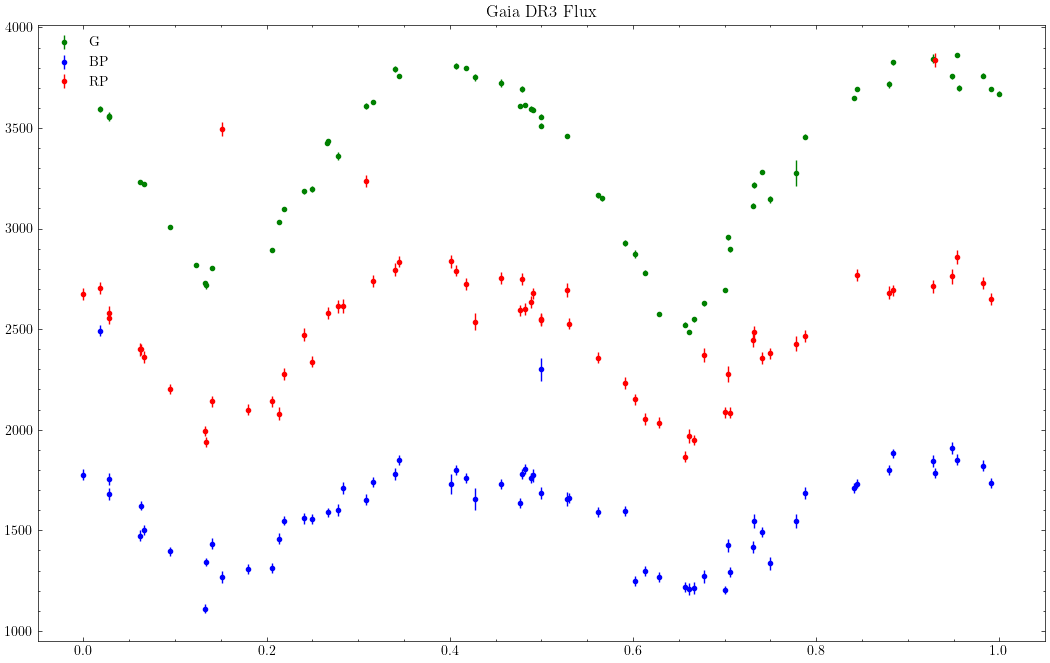
\includegraphics[scale=0.3]{Metodologia/Secciones/NormalizacionFlujos/Figures/GDR3 Flux.png}
	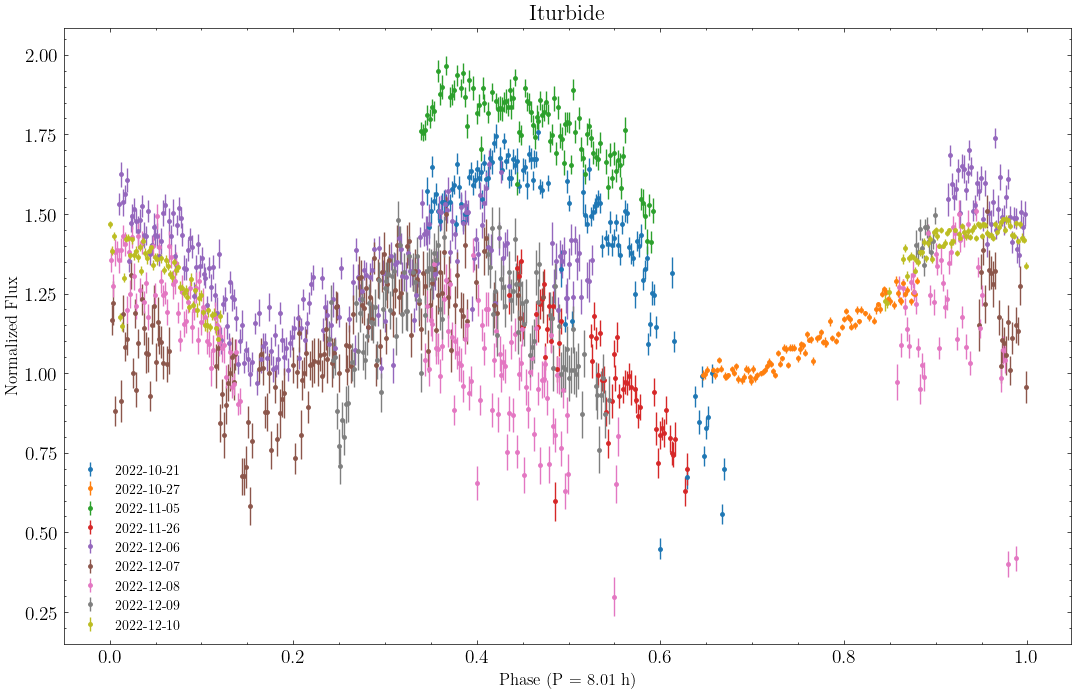
\includegraphics[scale=0.4]{Metodologia/Secciones/NormalizacionFlujos/Figures/Iturbide Normalized Flux.png}

	\caption{Flujo en fase de cada curva de luz utilizada. El catálogo de Gaia
		DR3 ya tiene reportado el flujo del sistema, por lo cual este se utilizó
		para el modelo en vez de obtener un flujo normalizado partiendo de las
		magnitudes.}
	\label{normFlujosCurvas}
\end{figure}
\chapter{Modelo Computacional} \label{metodologia:modelocomputacional}

Usando todas las curvas de luz disponible para el sistema \atoObjId se puede
generar un modelo computacional cuyos parámetros físicos resultan en una curva
de luz sintética que explique de manera adecuada las curvas fotométricas
observadas. Este método al final daría como resultado una \textit{solución
fotométrica} del sistema, en el cual se reportan los valores óptimos de cada
parámetro y la incertidumbre dada por la calidad de los datos. A continuación se
plasma el proceso que se llevó a cabo para llegar a una solución fotométrica del
sistema \atoObjIdNoSpace; debido a la alta dimensionalidad del problema de
sistemas binarios estelares, no se puede garantizar que esta sea la única
combinación de parámetros que mejor ajusten el modelo a los datos, aunque esta
posibilidad es mitigada utilizando las herramientas disponibles en PHOEBE.

\section{Preparación del Modelo}

El modelo en PHOEBE (llamado \textit{bundle} en inglés por el nombre de la clase
\code{phoebe.Bundle}) necesita ser preparado al principio para empezar el
proceso de ajuste. Esto incluye cargar las curvas fotométricas observadas de
cada catálogo al bundle; PHOEBE requiere que estas sean en arreglos de tiempo,
flujos, y errores de flujo\textemdash las mediciones de flujo se deben a que
PHOEBE no trabaja de manera directa con magnitudes, y los errores son necesarios
para que las herramientas de optimización de parámetros puedan funcionar
adecuadamente. En el Notebook
\href{https://github.com/KnightIV/UANL_MAPTA_Observaciones/blob/main/analisis/phoebe_model/initial-model-prep.ipynb}{\code{initial-model-prep.ipynb}}
está el código que se utilizó para cargar los datos de Iturbide, Gaia, y ZTF al
bundle en el que se trabajó; esto incluye realizar una limpieza de las curvas de
luz. Esto es más evidente en las curvas de luz en fase vistas en la
\reffigure{figuraGaiaIturbideZtfCurvasFase} donde se aprecia que varias
observaciones quedan fuera de la forma general aparente de su curva de luz
respectiva. Las observaciones más erróneas se pueden eliminar utilizando las
banderas (\textit{flags} como se identifican en los datos) que marcan los
problemas que sucedieron durante las observaciones. Para los pocos puntos que
quedaron fuera del rango de la curva de luz promedio se utilizaron límites de
flujo manuales en base a las gráficas vistas en la
\reffigure{figuraGaiaIturbideZtfCurvasFase}. Cada punto contribuye al cálculo de
la función de costo que parametriza la calidad del ajuste, por lo cual es
importante eliminar aquellos datos que tendrían un efecto negativo
significativo, afectando algoritmos que buscan optimizar el valor de esta
función.

Una optimización empleada en el cómputo del modelo hacia adelante es limitar los
puntos de tiempo para el cual se calcula el flujo recibido del sistema. Esto es
necesario para limitar el tiempo de ejecución del programa, en particular para
los procesos de optimización y muestreo MCMC que corren por varias iteraciones,
calculando el modelo sintético en cada iteración. PHOEBE utiliza los valores de
los tiempos de las curvas de luz proporcionadas para calcular el modelo hacia
adelante, lo cual causa que el modelo tarde varios minutos para generar la curva
sintética. Para declarar las fases de cómputo de manera explicita se utiliza el
siguiente código (implementado en el Notebook
\href{https://github.com/KnightIV/UANL_MAPTA_PlanObservaciones/blob/main/analisis/phoebe_model/estimations/ebai-default.ipynb}{\code{ebai-default.ipynb}}),
visto en la \refcode{codigoOptimizandoFasesComputoPhoebe}. El cálculo del modelo
hacia adelante en PHOEBE es en función de tiempo, no de fase, por lo cual PHOEBE
genera una lista de tiempos para el cual computar el modelo utilizando la
función \code{phases\_to\_times}, tomando como argumentos el periodo del
sistema, el tiempo de conjunción superior, y el cambio del periodo orbital con
el tiempo ($\mathrm{d}P_{\mathrm{orb}} / \mathrm{d}t$) en el caso de ser
distinto a 0. Los tiempos generados por esta función no se transforman a los
tiempos de las observaciones, pero debido a que el modelo sintético es evaluado
únicamente en fase esto no es un requisito importante para este estudio. El
tiempo de cómputo para el modelo hacia adelante de las curvas de ZTF:g y ZTF:r
se redujo de 10 minutos por modelo a aproximadamente 1 minuto por modelo.

\begin{figure}[!ht]
    \begin{lstlisting}[language=Python, autogobble]
        import phoebe

        # b: phoebe.Bundle
        b.flip_constraint('compute_phases@lcZtfG', 
            solve_for='compute_times@lcZtfG')
        b.set_value(qualifier='compute_phases', 
            dataset='lcZtfG', 
            value=phoebe.linspace(-0.5, 0.5, num=151, endpoint=True))
    \end{lstlisting}
    \caption{Estableciendo valores fijos de las fases orbitales para cuales
    calcular el modelo hacia adelante para la curva de luz \code{lcZtfG} en la
    pasabanda ZTF:g. La función \code{phoebe.linspace} genera una lista de
    valores numéricos en el intervalo $[-0.5, 0.5]$ de 151 elementos, una
    disminución significativa de los 453 puntos de tiempo en la curva observada
    de ZTF:g.}
    \label{codigoOptimizandoFasesComputoPhoebe}
\end{figure}

\section{Estimaciones Iniciales}

Una vez determinado el periodo orbital del sistema se puede empezar un estudio
de la morfología de las curvas de luz en fase, cuya forma se relaciona
directamente con parámetros físicos del sistema. PHOEBE ofrece distintos métodos
para generar las primeras estimaciones de los parámetros del sistema. El
estimador \textbf{EBAI-KNN} (descrito en la
\refthesissubsubsection{intro:phoebe:problema_inverso:ebai}) es capaz de estimar
los siguientes parámetros: el \textit{tiempo de conjunción superior}
(\code{t0\_supconj}), la \textit{razón de temperaturas} (\code{teffratio}), la
\textit{inclinación orbital} (\code{incl@binary}), el \textit{factor de relleno}
(\textit{fillout factor} en inglés, \code{fillout\_factor}), y la \textit{razón
de masas} (\code{q}). A pesar que dentro de PHOEBE estén implementados
estimadores adicionales, solo se puede aplicar el \textbf{EBAI-KNN} estimador;
esto se debe a que el modelo del sistema del que parte este trabajo corresponde
al de una binaria en contacto (elegido por la morfología aparente de la curva de
luz de Iturbide). Para poder adoptar los valores propuestos por los estimadores
fue necesario eliminar el constreñimiento puesto por PHOEBE en el parámetro
\code{fillout\_factor}. Este parámetro está constreñido por la función interna
de PHOEBE \code{pot\_to\_fillout\_factor}, la cual toma como entrada la razón de
masa \code{q} y el valor del potencial de Roche $\Omega$ que coincide con la
superficie delimitada por la envoltura común de una binaria en contacto. Como
resultado el parámetro \code{fillout\_factor} queda constreñido por los
parámetros \code{pot@contact\_envelope} y el radio de la estrella primaria
\code{requiv}, lo que efectivamente significa que los radios del sistema binario
quedan parametrizados por el factor de relleno. 

Dentro del Jupyter Notebook
\href{https://github.com/KnightIV/UANL_MAPTA_PlanObservaciones/blob/main/analisis/phoebe_model/estimations/ebai-default.ipynb}{\code{ebai-default.ipynb}}
se puede encontrar el código con el que se llevaron a cabo las pruebas de
estimación de parámetros. El estimador \textbf{EBAI-KNN} puede que obtenga
diferentes soluciones del sistema dependiendo de la curva de luz utilizada; por
lo cual se esperaba que obtuviera diferentes resultados dependiendo de las curvas
de entrada. Para obtener un panorama completo de las posibles soluciones
fotométricas se ejecutaron varios estimadores de PHOEBE, cada uno operando sobre
una diferente combinación de curvas de luz; se corrió un estimador por cada
curva de luz individual, al igual que unos estimadores que tuvieron de entrada
una combinación de curvas de luz de Gaia, Iturbide, y ZTF, con la finalidad de
experimentar con las capacidades de PHOEBE. El experimento completo junto a sus
curvas de luz sintéticas correspondientes se pueden ver en el Notebook
antes mencionado, acompañado de las gráficas resultantes de cada estimador.

\subsection{Elección del Modelo Inicial}

Una consideración importante en el proceso de modelación computacional es la
existencia de diferentes soluciones fotométricas dado un mismo conjunto de
datos. Esto se debe a la ortogonalidad de los parámetros en el sistema; dos o
más parámetros pueden estar correlacionados el uno al otro, lo cual significa
que no existe una solución única correcta del sistema. Para decidir entre los
varios estimadores se tomó como criterio de selección el ajuste del modelo hacia
adelante utilizando la métrica definida en la
\refequation{ecuacionLambdaCostoPhoebe}, $\lambda$, la cual está normalizada al
número de puntos en las curvas de luz observadas. Estos se pueden ver en la
\reffigure{figuraEstimadoresLambda}. Viendo solo la medida del ajuste $\lambda$
total para cada modelo se llegaría a la conclusión que el modelo
\code{ebai\_knn\_ztf\_solution} es el que más coincide con los datos
observacionales. Sin embargo, es necesario no solo ver el ajuste a cada curva de
luz individual, pero también considerar los valores físicos obtenidos del
estimador. Un criterio que empleamos fue adoptar la solución cuya razón de masa
\code{q} sea la más cercana al valor obtenido utilizando la red neuronal
desarrollada por
\citeyearparen{poro_investigation_of_orbital_period_mass_relations_2022}. Dado
el periodo orbital de $8.01 \ \mathrm{d}$ obtenemos un valor estimado de
aproximadamente $0.692$; de este se obtiene $1/q \approx 1.444$, el cual es
importante tener en mente ya que \code{q} en PHOEBE no está restringido al
intervalo $(0, 1]$ como en el modelo de
\citeyearparen{poro_investigation_of_orbital_period_mass_relations_2022}. Por lo
tanto se eligió las estimaciones de \code{ebai\_knn\_ztf\_gaia\_solution}, el
cual utilizó la fotometría de Gaia y ZTF.El resultado inicial del modelo se
puede ver en la \reffigure{figuraEstimacionInicialModelo}, junto a los
parámetros del modelo en la \reftable{ebaiKnnInitialEstimationsValues}.

\begin{figure}[!ht]
	\centering
	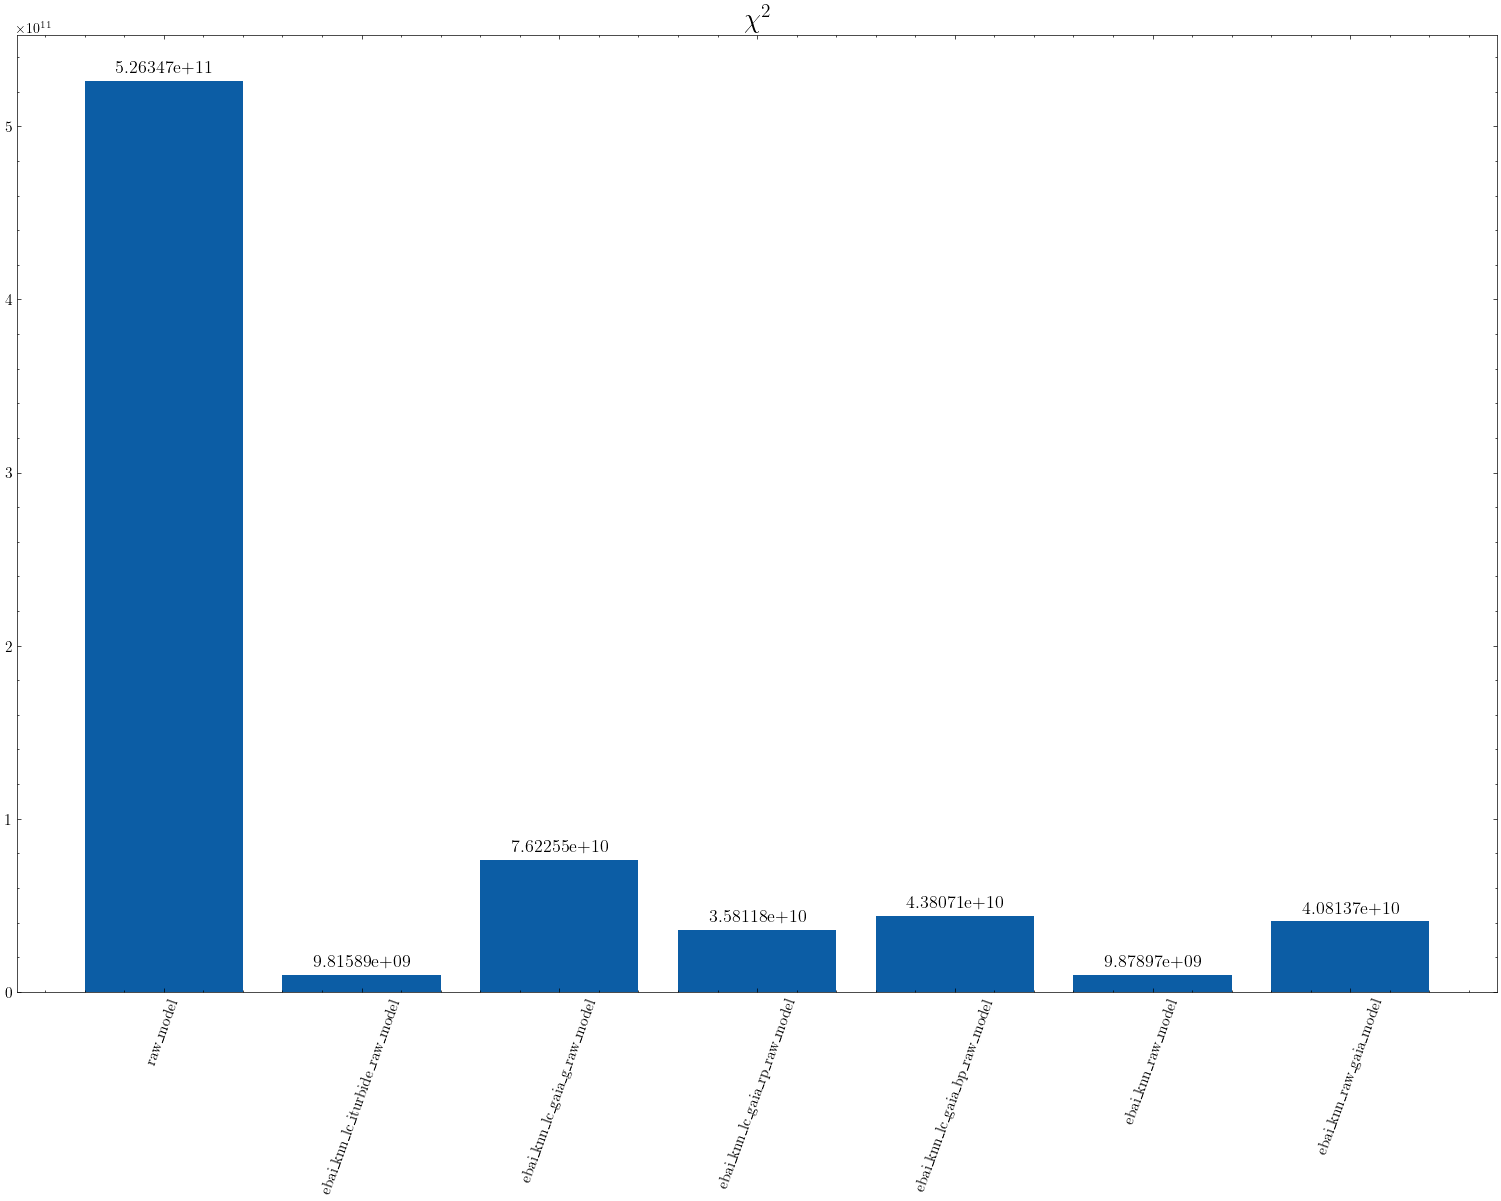
\includegraphics[scale=0.6]{Metodologia/Secciones/ModeloComputacional/Figures/EstimadoresChiResultados.png}

	\caption{Resultados del ajuste ($\lambda$) de los modelos sintéticos
		generados utilizando los parámetros dados por cada estimador. Cada
		estadística fue calculada con respecto a todos los datos observacionales
		disponibles, sin importar las combinaciones de curvas de luz utilizadas
		para hacer la estimación. \code{default\_model} corresponde al modelo
		inicial que ofrece PHOEBE a través de la función
		\code{phoebe.default\_contact\_binary()}. Los nombres de los estimadores
		en el eje vertical de la gráfica indican los datos observacionales
		utilizados para cada estimación de parámetros, junto al valor del ajuste
		el modelo sintético a todas las curvas del modelo. }
	\label{figuraEstimadoresLambda}
\end{figure}

\begin{figure}[!ht]
	\centering
	\xincludegraphics[scale=0.41]{Metodologia/Secciones/ModeloComputacional/Figures/ebaiKnnIturbideNorm.png}
	\xincludegraphics[scale=0.41]{Metodologia/Secciones/ModeloComputacional/Figures/ebaiKnnGaiaRaw.png}
	\xincludegraphics[scale=0.41]{Metodologia/Secciones/ModeloComputacional/Figures/ebaiKnnZtf.png}

	\caption{Modelos sintéticos del modelo utilizando los parámetros estimados
	por \code{ebai\_knn\_ztf\_gaia\_solver} junto a los residuos en los flujos
	para cada curva de luz. Estos modelos fueron sintetizados utilizando un
	factor de escala de flujos flexible, utilizando la opción \code{pblum\_mode
	= "dataset\_scaled"}, el cual nos permite analizar la morfología del modelo
	sintético sin considerar por ahora el efecto en la escala de la curva de
	parámetros relacionados con la luminosidad de cada componente, como las
	temperaturas absolutas o los radios de ambas estrellas. Estos parámetros son
	ajustados en los siguientes pasos de afinación del modelo.}
	\label{figuraEstimacionInicialModelo}
\end{figure}

% TODO: style table
\begin{table}[!ht]
	\centering
	\begin{tabular}{|l|l|}
		\hline
		% \rowcolor{blue}
		\thead{Parámetro}                        & \thead{Valor} \\
		\hline
		\code{t0\_supconj@binary}                & 0.02571 d    \\
		\hline
		\code{teffratio@binary}                  & 0.98746       \\
		\hline
		\code{incl@binary}                       & 70.3197 deg  \\
		\hline
		\code{fillout\_factor@contact\_envelope} & 0.25767       \\
		\hline
		\code{q@binary}                          & 1.93380       \\
		\hline
	\end{tabular}
	\caption{Resultados adoptados de las estimaciones iniciales, utilizando el
		estimador cuyos datos de entrada fueron las curvas de Gaia y ZTF. Las
		unidades de cada valor son especificadas excepto para los parámetros
		adimensionales.}
	\label{ebaiKnnInitialEstimationsValues}
\end{table}

\section{Optimización de Parámetros}

Como se puede ver en la \reffigure{figuraEstimacionInicialModelo} el modelo
inicial de PHOEBE no se ajusta perfectamente bien a los datos
observacionales, visto en los residuos de cada curva de luz. En la siguiente
etapa del proyecto se emplea un muestreo MCMC, el cual en teoría es capaz de
determinar el mínimo global del espacio de parámetros, pero a un costo
computacional que crece exponencialmente con la distancia de los parámetros del
sistema actuales al mínimo global de la función de calidad.

El proceso de optimización de parámetros es distinto para cada sistema modelado;
ciertas estrategias pueden funcionar para un sistema y al mismo tiempo no llegar
a una solución adecuada para otro sistema con distintos datos. Para el ajuste de
\atoObjId primero se ajustó el tiempo de superconjunción; esto es visto en los
eclipses del modelo sintético desfasado con los eclipses de las curvas
observadas en la \reffigure{figuraEstimacionInicialModelo}. Esto resultó en un
nuevo valor de $0.02589 \ \mathrm{d}$. Utilizando un optimizador de Nelder Mead
Simplex (\textit{NMS}, descrito en la
\refthesissubsubsection{intro:phoebe:nelder_mead}) se buscó optimizar los mismos
parámetros configurados en la estimación inicial del modelo. Con la finalidad de
obtener un ajuste consistente y solo utilizar datos de alta calidad solo se
utilizó las dos curvas de luz de ZTF para el resto del ajuste del modelo. Esto
se debe al número de buenas observaciones en estos datos; son más numerosas de
las observaciones hechas por Gaia, y son de mejor calidad que las realizadas
desde el OAU. Al tener observaciones simultaneas en diferentes pasabandas
también es posible determinar las temperaturas efectivas de las componentes
estelares. 

El primer optimizador NMS corrigió la razón de temperaturas efectivas
\code{teffratio} (el cual sirve para modificar la luminosidad relativa de la
estrella secundaria con respecto a la primaria, ajustando la profundidad del
eclipse secundario con respecto al eclipse primario), el factor de relleno
\code{fillout\_factor} (que sirve como una parametrización de la razón de radios
de las estrellas, ajustando el ancho de ambos eclipses), la inclinación orbital
del sistema \code{incl@binary} (que dicta el aspecto de los eclipses observados
con respecto al plano de observación, determinando la profundidad y la agudeza
de los eclipses), y la razón de masa \code{q}. La razón de masa no es un
parámetro que se pueda constreñir bien utilizando solo información fotométrica;
esto se debe a las correlaciones presentes en el modelo con los demás parámetros
del sistema. Después de 114 iteraciones el optimizador logró converger a una
solución dada en la \reftable{tablaOptNmResultados}.

% TODO: style table
\begin{table}[!ht]
	\centering
	\begin{tabular}{|l|l|}
		\hline
		% \rowcolor{blue}
		\thead{Parámetro}                        & \thead{Valor optimizado} \\
		\hline
		\code{teffratio@binary}                  & 1.07991       \\
		\hline
		\code{incl@binary}                       & 70.19810 deg  \\
		\hline
		\code{fillout\_factor@contact\_envelope} & 0.09356       \\
		\hline
		\code{q@binary}                          & 2.13478       \\
		\hline
	\end{tabular}
	\caption{Valores optimizados utilizando el algoritmo Nelder-Mead Simplex.}
	\label{tablaOptNmResultados}
\end{table}

\begin{figure}
	\centering
	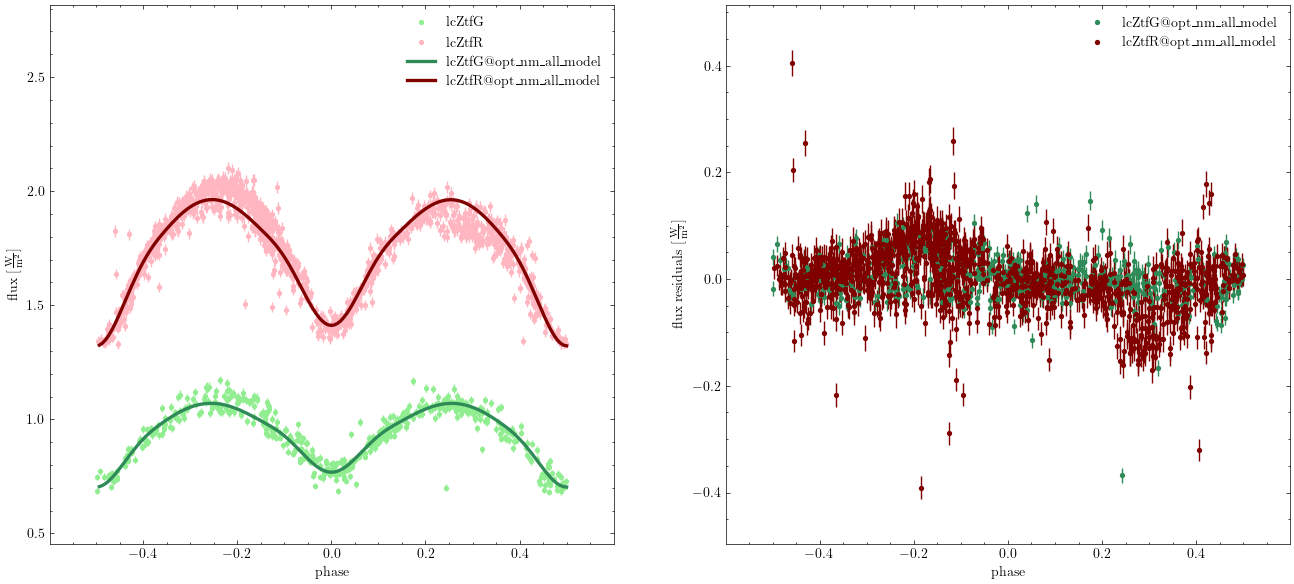
\includegraphics[scale=0.5]{Metodologia/Secciones/ModeloComputacional/Figures/Figura Opt NM Resultados ZTF.png}
	\caption{Modelo sintético generado utilizando los parámetros dados por el
	optimizador NMS, vistos en la \reftable{tablaOptNmResultados}, utilizando el
	tiempo de superconjunción corregido.}
	\label{figuraOptNmResultadosZtf}
\end{figure}

La curva sintética del modelo optimizado visto en la
\reffigure{figuraOptNmResultadosZtf} muestra una asimetría en las jorobas de la
curva de luz en fase. Estos máximos corresponden a las fases orbitales en las
cuales la mayor cantidad de elementos superficiales de ambas componentes
coinciden con nuestra línea de observación. Este fenómeno se le denomina el
\textit{efecto O'Connell}, descrito originalmente por
\citeyearparen{oconnell_periastron_effect-OConnell_effect_1951} donde se
distingue del efecto de periastro que es causado por efectos de marea en
sistemas con órbitas excéntricas. El \textit{efecto O'Connell} se debe a la
diferencia de luminosidad entre diferentes hemisferios de una estrella; puede
ser causado por un punto caliente debido a la acreción de material en el caso de
haber una alta tasa de transferencia de masa
[\citeyearparen{darwish_light_curve_analysis_four_new_short_period_eclipsing_binaries_2024}],
o por manchas en la superficie estelar debido a actividad en la fotósfera. Para
llegar a un mejor ajuste de la curva fotométrica se introdujo una mancha fría en
la estrella secundaria. Después de hacer un ajuste manual de los parámetros de
la mancha se utilizó un optimizador NMS para obtener los parámetros óptimos de
la mancha estelar. Los parámetros optimizados se pueden ver en la
\reftable{tablaOptManchaResultados}, y la mancha estelar se puede ver
representada en la \reffigure{figuraMallaManchaNm}.

% TODO: style table
\begin{table}[!ht]
	\centering
	\begin{tabular}{|l|l|}
		\hline
		% \rowcolor{blue}
		\thead{Parámetro}	& \thead{Valor optimizado} \\
		\hline
		\code{colat}	& 89.77983 deg	\\
		\hline
		\code{long}		& 81.09966 deg  \\
		\hline
		\code{radius} 	& 25.12086 deg	\\
		\hline
		\code{relteff}	& 0.93007		\\
		\hline
	\end{tabular}
	\caption{Parámetros de la mancha estelar optimizados utilizando el algoritmo
	Nelder-Mead Simplex, el cual logró converger después de 102 iteraciones.
	Todos los parámetros son relativos a la superficie estelar a la que le
	pertenece la mancha; la longitud \code{long} donde se define la longitud
	$0^{\circ}$ viendo a la estrella primaria, la latitud \code{colat} se define
	como el ángulo polar empezando desde el polo norte de la estrella, el radio
	angular \code{radius}, y la temperatura efectiva relativa \code{relteff} con
	respecto a la temperatura superficial.}
	\label{tablaOptManchaResultados}
\end{table}

\begin{figure}[!ht]
	\centering
	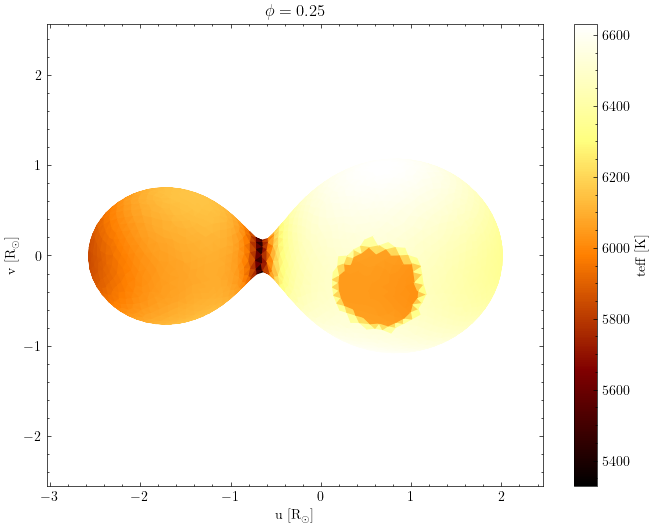
\includegraphics[scale=0.8]{Metodologia/Secciones/ModeloComputacional/Figures/Figura Malla Mancha NM.png}
	\caption{Malla representando la superficie estelar de ambas componentes en
	su fase orbital $\phi = 0.25$, en el máximo menor de la curva fotométrica.
	Aquí se puede apreciar la mancha estelar introducida a la componente
	secundaria. La temperatura efectiva de cada elemento superficial de la
	envoltura en común, donde la mancha se ve de un color más oscuro debido a su
	baja temperatura con respecto al resto de la superficie estelar.}
	\label{figuraMallaManchaNm}
\end{figure}

Una vez que se haya llegado a un nivel de ajuste adecuado con los optimizadores
de tipo NMS se aplicó un último ajuste utilizando correcciones diferenciales,
los cuales funcionan mejor cuando los parámetros se encuentren lo
suficientemente cerca del mínimo global, para evitar caer y estar atrapados
dentro de un mínimo local. El motivo para acercarnos lo más posible al mínimo
global es para reducir el trabajo del muestreo MCMC; entre mayor sea la
distancia que los caminadores tengan que recorrer, se requerirá más iteraciones
para obtener un muestreo adecuado del espacio de parámetros. El resolvedor se
crea con el código en la \refcode{codigoOptimizadorDc}, en donde se define el
tamaño de los pasos que intenta hacer el optimizador; estos deben de ser
suficientemente pequeños para evitar saltos fuera del área de interés, pero
suficientemente grandes para que haya un cambio en el ajuste del modelo. El
tamaño de los pasos se determinó por medio de experimentación manual del efecto
en un modelo sintético de PHOEBE.

\begin{figure}[!ht]
	\begin{lstlisting}[language=Python, autogobble]
		b.add_solver('optimizer.differential_corrections', solver='dc_relative', overwrite=True,
             fit_parameters=['teffratio', 'incl@binary', 'fillout_factor', 'q'],
             steps={
                'q': 0.01,
                'incl@binary': 1,
                'fillout_factor': 0.01,
                'teffratio': 0.01
             })
	\end{lstlisting}
	\caption{Código que se utilizó para crear el optimizador de correcciones
	diferenciales para los parámetros que dictan la forma de la curva de luz en
	fase. El argumento \code{steps} del optimizador representa $\Delta
	\mathbf{p} = \{ \Delta p_1, ..., \Delta p_k \}$ visto en la
	\refequation{ecuacionDiferenciasFinitas}.}
	\label{codigoOptimizadorDc}
\end{figure}

% TODO: style table
\begin{table}[!ht]
	\centering
	\begin{tabular}{|l|l|}
		\hline
		% \rowcolor{blue}
		\thead{Parámetro}                        & \thead{Valor optimizado} \\
		\hline
		\code{teffratio@binary}                  & 1.06676       \\
		\hline
		\code{incl@binary}                       & 68.42157 deg  \\
		\hline
		\code{fillout\_factor@contact\_envelope} & 0.07892       \\
		\hline
		\code{q@binary}                          & 1.10457       \\
		\hline
	\end{tabular}
	\caption{Valores optimizados utilizando un optimizador de correcciones diferenciales.}
	\label{tablaOptDcResultados}
\end{table}

Después de 17 iteración se obtuvieron los parámetros vistos en la
\reftable{tablaOptDcResultados}, de los cuales se generó las curvas sintéticas
vistas en la \reffigure{figuraOptDcResultadosZtf}. El optimizador de
correcciones diferenciales no se utilizó para ajustar los parámetros de la
mancha estelar; estos se mantuvieron fijos en sus valores determinados por el
optimizador NMS para después explorar utilizando MCMC.

\begin{figure}[!ht]
	\centering
	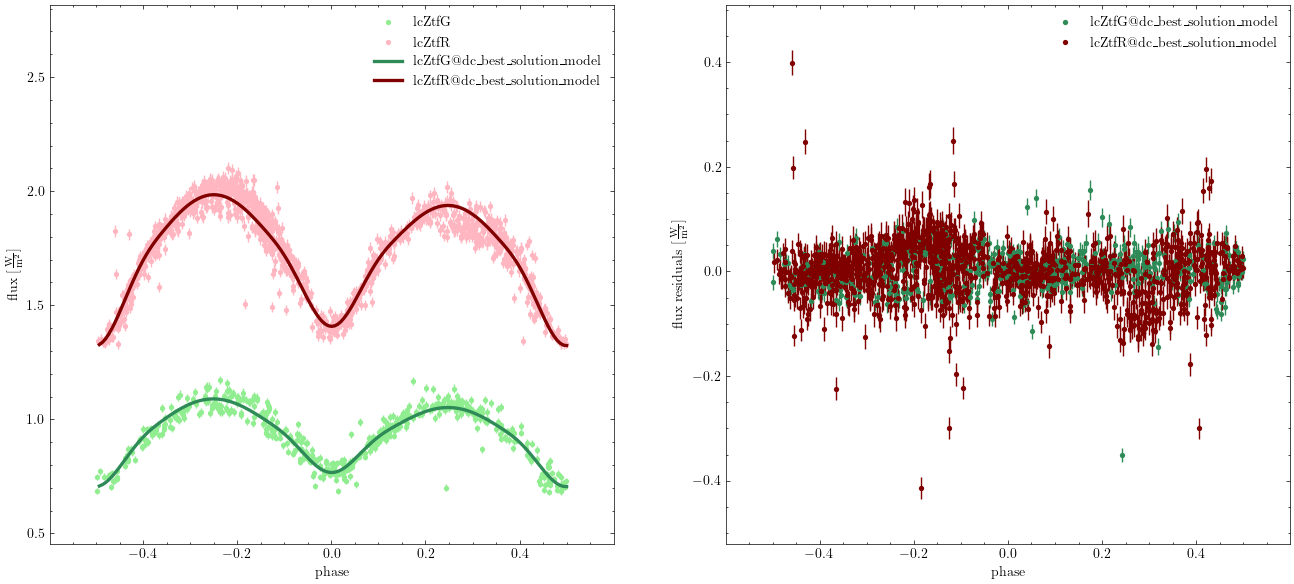
\includegraphics[scale=0.5]{Metodologia/Secciones/ModeloComputacional/Figures/Figura Opt DC Resultados ZTF.png}
	\caption{Modelo sintético junto a el residuo de flujo tomando en cuenta una
	mancha estelar fría en la componente secundaria (vista en la
	\reffigure{figuraMallaManchaNm}) y utilizando los parámetros resultados del
	proceso de optimización vistos en la \reftable{tablaOptDcResultados}.}
	\label{figuraOptDcResultadosZtf}
\end{figure}

\section{Ajuste de Luminosidad y Temperatura Efectiva}

Utilizando las curvas calibradas de ZTF en ambas pasabandas se determinó la
temperatura efectiva del sistema partiendo unicamente de las curvas
fotométricas. Para esto se manipularon en total 3 parámetros del sistema: la
temperatura efectiva de la componente primaria (\code{teff@primary}), la razón
de temperaturas de las componentes $T_2 / T_1$ (\code{teffratio}), y el factor
de escala de la luminosidad de pasabanda (\code{pblum@primary@lcZtfG}) para la
pasabanda ZTF:g. Se acopló la temperatura efectiva del sistema al color (dado
por el flujo relativo entre las curvas de ZTF) utilizando el modo
\code{pblum\_mode} con el valor \code{component-coupled} para la curva de ZTF:g,
y un valor de \code{dataset-coupled} para la curva de ZTF:r. En el modo
\code{component-coupled} el usuario proporciona un valor para la luminosidad
emergente de la componente primaria en el tiempo $t_0$ del sistema, a partir del
cual PHOEBE determina un factor de escala tal que las intensidades superficiales
de las estrellas sean igual a la luminosidad dada. El modo
\code{dataset-coupled} aplica el mismo factor de escala a la curva de ZTF:r que
el factor dado a la curva ZTF:g, manteniendo información del color del sistema
[\citeyearparen{conroy_phoebe_v_framework_solving_inverse_problem_2020}]. 

Una vez que se haya establecido esta configuración del bundle se aplicó un
optimizador de tipo NMS para ajustar los tres parámetros mencionados en el
párrafo pasado. Como valor inicial se ajustó manualmente la temperatura efectiva
de la primaria a $4600 \ \mathrm{K}$, el cual se determinó por medio de
experimentación manual. Después de 174 iteraciones el optimizador logró
converger a la solución dada en la \reftable{tablaOptNmTeffResultados}. Dado que
estos parámetros principalmente afectan el factor de escala de las curvas de
luz, los demás parámetros del sistema se mantuvieron fijos, manteniendo la forma
de las curvas de luz.

% TODO: style table
\begin{table}[!ht]
	\centering
	\begin{tabular}{|l|l|}
		\hline
		% \rowcolor{blue}
		\thead{Parámetro}                        & \thead{Valor optimizado} \\
		\hline
		\code{teff@primary}							& 4203.69115 K  \\
		\hline
		\code{teffratio@binary}						& 1.05213       \\
		\hline
		\code{pblum@primary@lcZtfG}					& 4.78643 W       \\
		\hline
	\end{tabular}
	\caption{Valores optimizados para la temperatura efectiva de la estrella
	primaria, junto a la luminosidad de pasabanda que produce el factor de
	escala necesario para ajustar a la curva fotométrica. La temperatura
	efectiva de la secundaria está constreñida por la temperatura efectiva de la
	primaria y la razón de temperaturas; dado estos parámetros, la temperatura
	efectiva secundaria es igual a 4422.837561158592 K.}
	\label{tablaOptNmTeffResultados}
\end{table}

\section{Muestreo MCMC}

Una vez que se haya obtenido el conjunto de parámetros que mejor ajustan el
modelo sintético a los datos observacionales se busca obtener las incertidumbres
para cada parámetro. La manera recomendada por el equipo de desarrollo de PHOEBE
es por medio de un muestreo Bayesiano \textit{Monte Carlo Markov Chain}.
Utilizando un muestreo MCMC es posible determinar la morfología del espacio de
parámetros de manera holística; esto permite identificar cualquier correlación
que exista entre los parámetros del sistema. El proceso de muestreo empleado en
este proyecto es por PHOEBE utilizando el paquete de Python \code{emcee},
descrito en la \refthesissubsection{intro:phoebe:problema_inverso:muestreo}.
Antes de correr el proceso de muestreo se preparó el bundle de la siguiente
manera.

\subsection{Eliminación de Observaciones Erróneas}

PHOEBE utiliza la probabilidad logarítmica ($\mathrm{lnprobability}$) del modelo
sintético como la \textit{función de merito} para el muestreo. Esta se define en
la siguiente ecuación:

\begin{eqfloat}[!ht]
	\centering
	\begin{equation}
		\textrm{lnprobability} = \textrm{lnpriors} + \textrm{lnlikelihood}
	\end{equation}
\end{eqfloat}

Donde $\mathrm{lnpriors} = \sum_{\Pi} \ln{P(p | \pi)}$ es la probabilidad
logarítmica de obtener los parámetros actuales del modelo $p$ de una
distribución a priori $\pi$ sumando sobre todas las distribuciones priores $\Pi$
[\citeyearparen{conroy_phoebe_v_framework_solving_inverse_problem_2020}]. El
término $\mathrm{lnlikelihood}$ es la verosimilitud, la cual está definido por
la \refequation{ecuacionLnLikelihoodMcmc}. Tras varios experimentos corriendo
varias instancias del muestreo MCMC se descubrió que los caminadores son
excepcionalmente sensibles a fluctuaciones en la función de merito; las
observaciones que se desvían de manera significativa de la región principal de
la curva de luz en fase indican un ajuste inadecuado según la función de merito.
Debido a que las incertidumbres de estos puntos probablemente fueron registrados
de manera errónea se eliminaron estos puntos de la curva observada. En el
Notebook
\href{https://github.com/KnightIV/UANL_MAPTA_Observaciones/blob/main/analisis/phoebe_model/sampling/remove-bad-observations.ipynb}{\code{remove-bad-observations.ipynb}}
se aplicó un criterio al desviación estándar de los residuos del modelo
optimizado; aquellos puntos cuya diferencia con el modelo sintético sea mayor de
un múltiple de la desviación estándar fue eliminado de los datos. Los resultados
de esta optimización se pueden ver en la
\reffigure{figuraEliminarMalasObservacionesZtf}. El modelo sintético utilizando
solo estos datos se puede ver en la
\reffigure{figuraModeloSinMalasObservacionesZtf}, donde se puede apreciar a
mayor detalle la forma oscilatoria de los residuos. Esto indica que los valores
obtenidos no son los óptimos y aún hay más cambios que se podrían emplear para
llegar a un mejor ajuste; sin embargo, este es un ajuste suficientemente bueno
para este proyecto para continuar al muestreo del espacio de parámetros con
MCMC.

\begin{figure}[!ht]
	\centering
	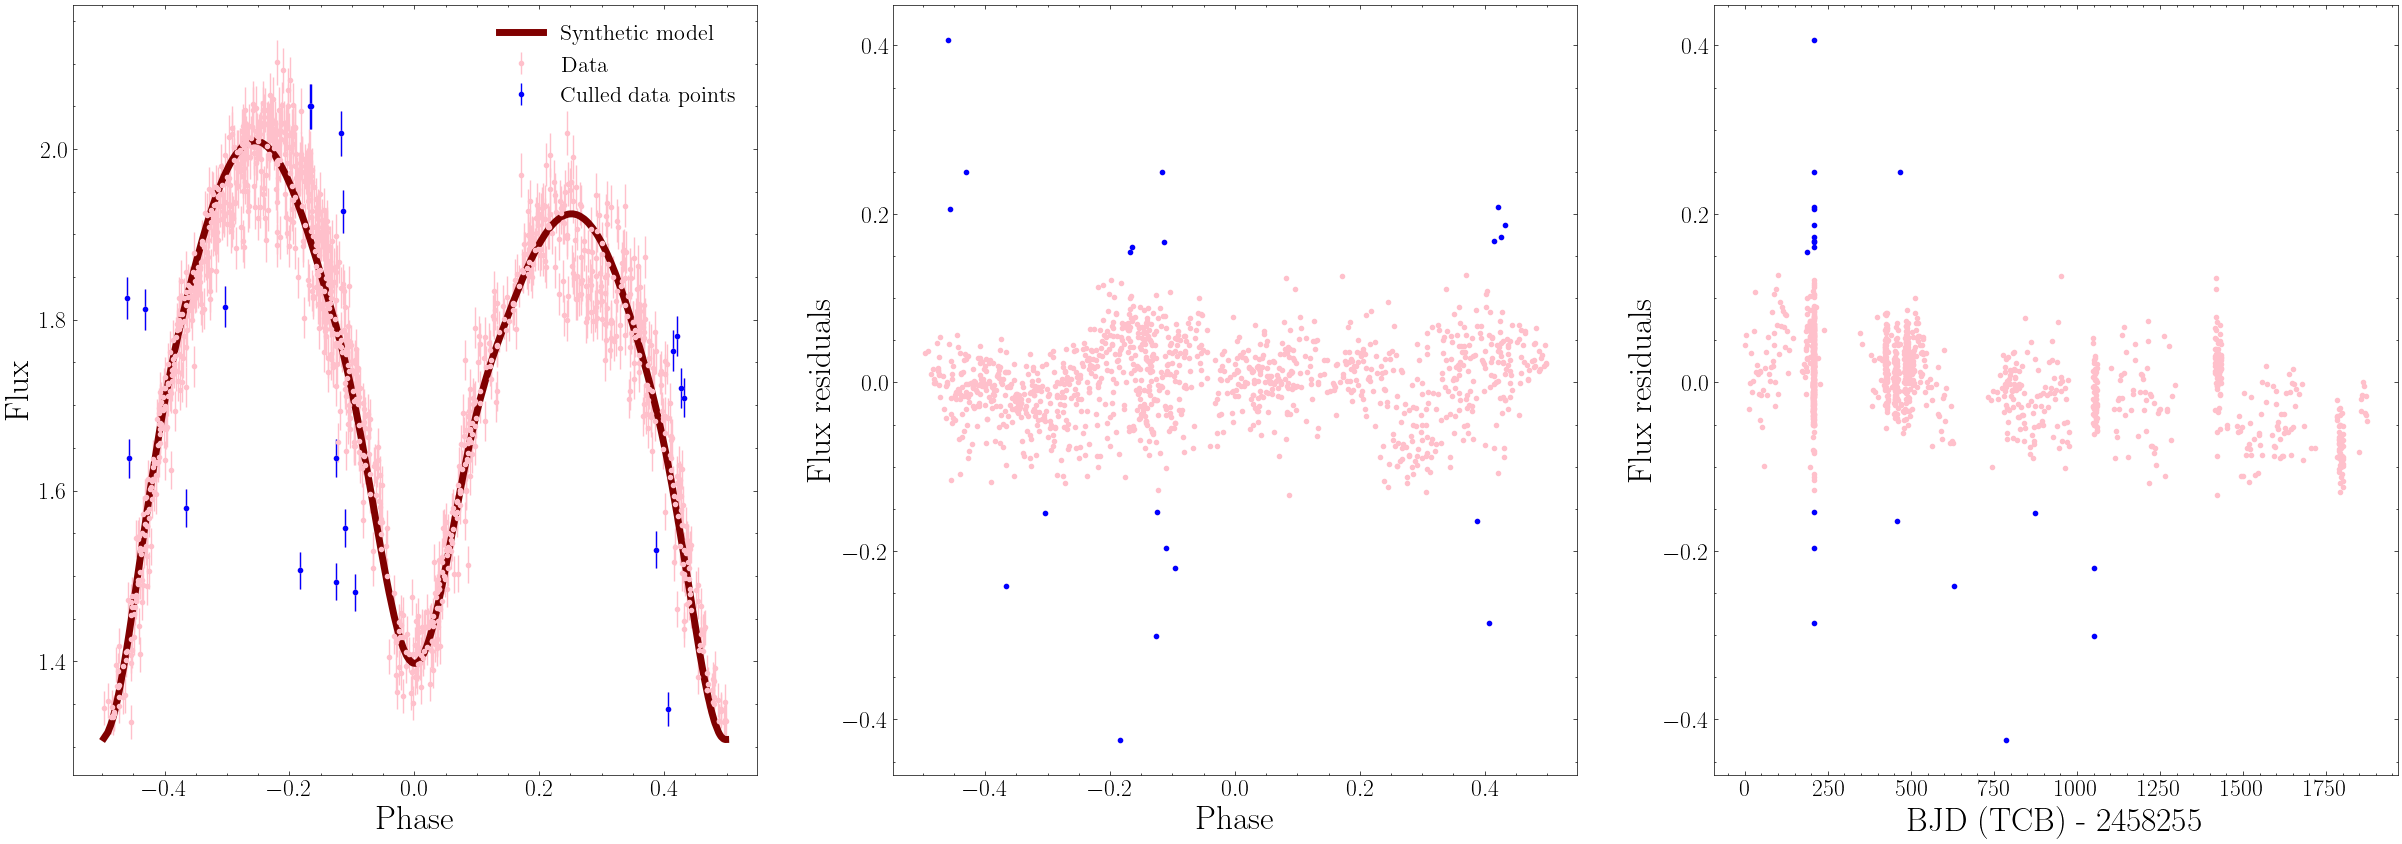
\includegraphics[scale=0.27]{Metodologia/Secciones/ModeloComputacional/Figures/Figura Malas Observaciones ZTF:r.png}
	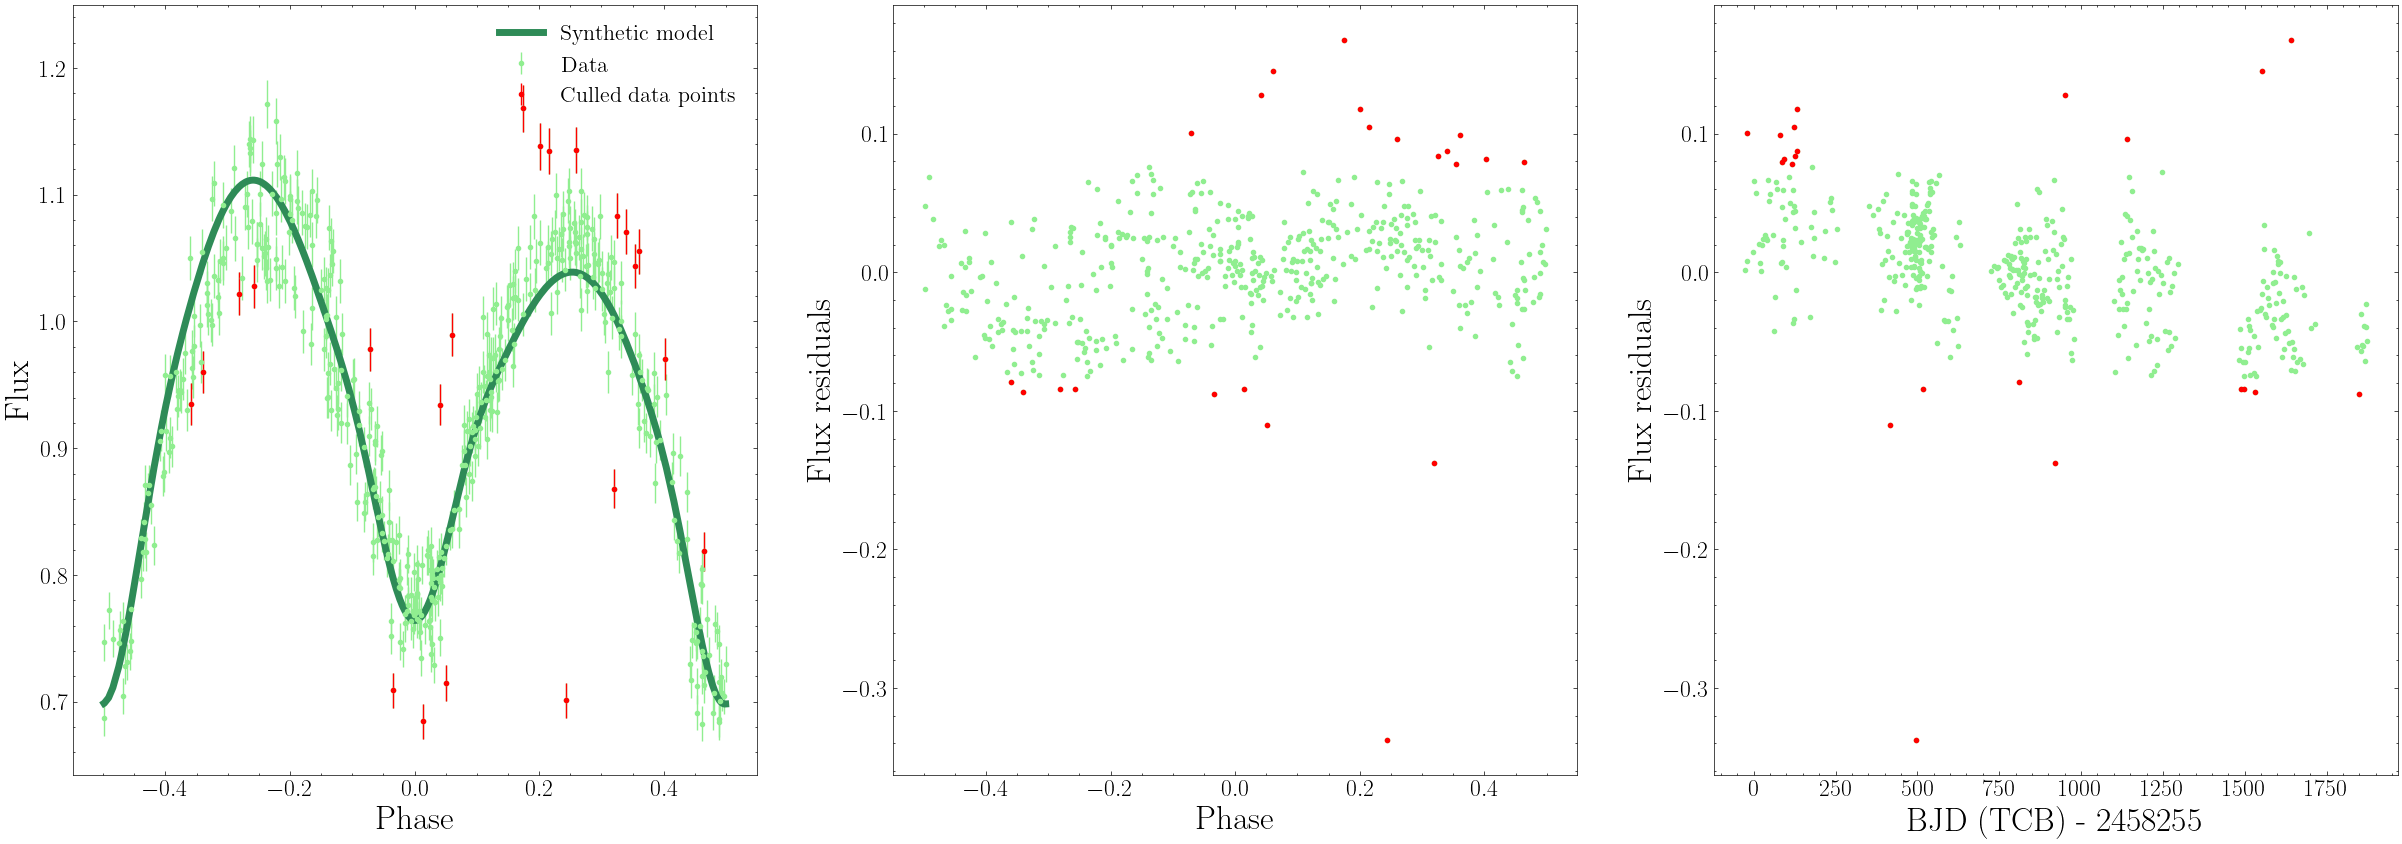
\includegraphics[scale=0.27]{Metodologia/Secciones/ModeloComputacional/Figures/Figura Malas Observaciones ZTF:g.png}
	\caption{Resultados de aplicar el criterio de eliminación para las curvas de
	luz de ZTF, donde la figura superior corresponde a la pasabanda ZTF:r y la
	inferior a ZTF:g. Se optó por codificar este criterio en el código en vez de
	eliminar los datos manualmente para ser fácilmente reproducible. El factor
	de escala del criterio fue ajustado manualmente tal que los puntos más
	erróneos sean eliminados con éxito, y al mismo tiempo preservar la forma y
	dispersión principal que existen en los datos.}
	\label{figuraEliminarMalasObservacionesZtf}
\end{figure}

\begin{figure}[!ht]
	\centering
	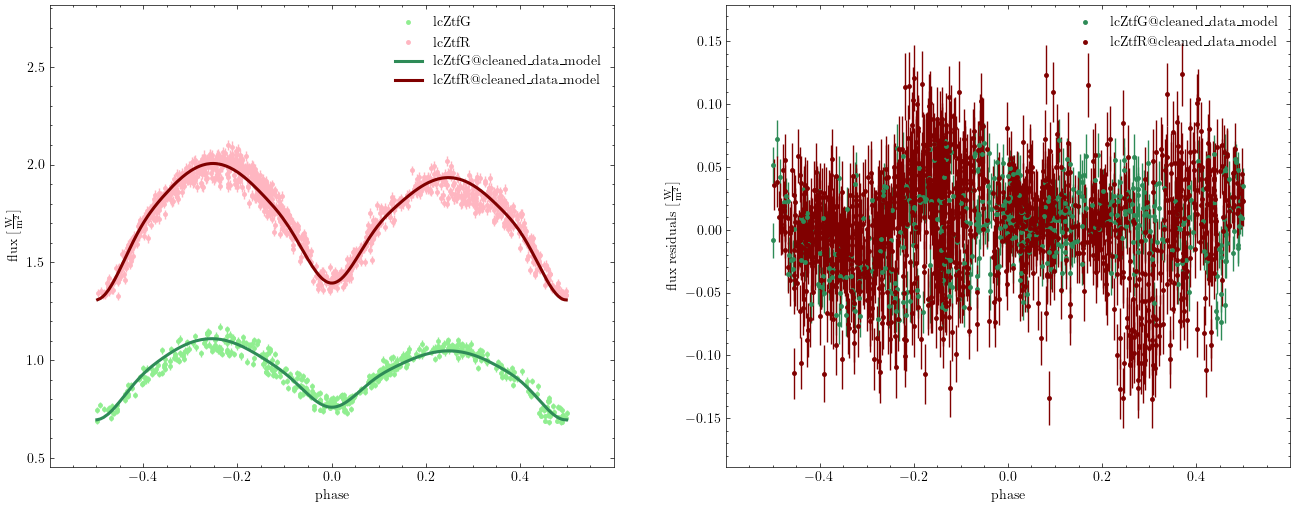
\includegraphics[scale=0.5]{Metodologia/Secciones/ModeloComputacional/Figures/Figura Modelo Sin Malas Observaciones ZTF.png}
	\caption{Modelo sintético en las pasabandas de ZTF calculado después de
	eliminar las observaciones más problemáticas de las curvas observadas.}
	\label{figuraModeloSinMalasObservacionesZtf}
\end{figure}

\subsection{Distribuciones Priores}

Para poder muestrear el espacio de parámetros, el algoritmo MCMC requiere de una
región inicial a partir de cual inicializar las posiciones de cada caminador.
Estas distribuciones iniciales también actúa como una guía; al principio del
muestreo los caminadores en su mayoría no saldrán de las regiones de
concentración de estas distribuciones. La forma de las priores dejará de
importar tanto entre más iteraciones logre correr la cadena, de la cual se
estimará la distribución posterior de densidad de cada parámetro.

PHOEBE ofrece unas herramientas para los tipos de distribuciones más comunes en
este trabajo: la distribución uniforme y la distribución Gaussiana (normal).
Para el muestreo de \atoObjId se utilizaron distribuciones uniformes para los
parámetros ajustables del bundle\textemdash todos aquellos que han sido
ajustados a lo largo de la optimización de parámetros. Una distribución uniforme
no tiene un significado físico intrínseco más allá de comunicar una falta de
información del problema. En nuestro caso, las priores sirven para marcar un
límite práctico para cada parámetro, tanto para evitar que los caminadores se
pierdan en espacios que produzcan un resultado no físico, cómo para constreñir
el volumen de interés a lo más cercano de los parámetros óptimos derivados en el
proceso de optimización. 

Se crearon 3 colecciones de distribuciones en el bundle de PHOEBE para delimitar
los parámetros ajustables del modelo: 1 para los parámetros de interés del
sistema binario, 1 para los parámetros que rigen la mancha estelar en la
componente secundaria, y 1 que restringe el factor de escala en la pasabanda
ZTF:g. Las colecciones individuales de distribuciones priores se pueden ver en
la \reffigure{figuraColeccionesPrioresZtf}, la
\refthesissection{apendice:modelo_computacional_graficas:dist_priores_completas}
muestra todos los priores utilizados para el proceso de MCMC.

\begin{figure}[!ht]
	\centering
	\xincludegraphics[scale=0.29, label=\textbf{(a)}, labelbox=true, pos=ne, fontsize=\Large]{Metodologia/Secciones/ModeloComputacional/Figures/Figura Prior Params Binaria.png}
	\xincludegraphics[scale=0.345, label=\textbf{(b)}, labelbox=true, pos=ne, fontsize=\Large]{Metodologia/Secciones/ModeloComputacional/Figures/Figura Prior Params Mancha.png}
	\xincludegraphics[scale=0.85, label=\textbf{(c)}, labelbox=true, pos=ne, fontsize=\Large]{Metodologia/Secciones/ModeloComputacional/Figures/Figura Prior Params Luminosidad ZTF.png}
	\caption{Distribuciones priores utilizadas como límites iniciales a cada
	caminador. Se separaron en 3 distintas colecciones por cuestiones de
	organización dentro del código: \textbf{(a)} los parámetros principales del
	sistema solar que afectan la forma de la curva fotométrica sintética en
	orden de izquierda a derecha y de arriba a abajo: la temperatura efectiva de
	la componente primaria ($T_{1}$), la razón de temperaturas ($T_2/T_1$), el
	factor de relleno ($f$), la inclinación orbital ($i_{\mathrm{orb}}$), y la
	razón de masas ($q$). \textbf{(b)} los parámetros de la mancha estelar en la
	componente secundaria que se introdujo para tomar en cuenta el efecto
	O'Connell: su posición con respecto al origen del sistema de coordenadas en
	la secundaria (la longitud y latitud de la mancha), el radio angular, y la
	razón de temperatura de la mancha con respecto a la temperatura efectiva
	local de la superficie de la componente secundaria. \textbf{(c)} la
	luminosidad en la pasabanda ZTF:g, la cual determina el factor de escala de
	las curvas de luz; este parámetro fue incluido en el muestreo para permitir
	integrar sobre este \textit{parámetro molesto}, ya que tiene un efecto
	significativo en la curva sintética pero no es un parámetro que nos interese
	medir directamente.}
	\label{figuraColeccionesPrioresZtf}
\end{figure}

\subsection{Inicializando el Muestreo MCMC}

Una vez que se hayan determinado las distribuciones priores que utilizar para
inicializar la cadena se puede empezar el muestreo. Se emplearon 160 caminadores
en total; en general, es mejor tener la mayor cantidad de caminadores posible
tal que sea mayor que la cantidad de parámetros que se van a explorar (10
parámetros vs. 160 caminadores). Esto también está restringido por el cómputo
disponible. El \textit{stretch-move} algoritmo descrito por
\citeyearparen{foreman-mackey_emcee_2013} muestra que un ensamble no es
completamente paralelizable, por lo tanto no es necesario restringir la cantidad
de caminadores estrictamente al número de procesadores (hilos) disponibles en
una computadora. 

El muestreo MCMC se corrió en un servidor propiedad del Dr. Carlos Esteban
Chávez Pech de la Facultad de Ingeniería Mecánica y Eléctrica en la Universidad
Autónoma de Nuevo León. Este servidor cuenta con 4 CPUs físicos AMD Opteron(tm)
Processor 6376, el cual suma a 64 procesadores virtuales disponibles al sistema
operativo (y por ende al código MCMC). La computadora está equipada con 32 GB de
memoria RAM\textemdash a pesar que el mayor costo del muestreo es en el cómputo
directo, la cantidad de memoria requerida aumenta rápidamente entre más
caminadores se utilizan debido a la copia de datos necesaria por el proceso de
paralelización por medio del módulo \code{multiprocessing} de Python. El
muestreo final de este trabajo utilizó 13 GB de memoria, el cual fue asignado
por el código al principio del proceso, manteniéndose estable por el resto del
tiempo de cómputo.

Para poder estar revisando el progreso del muestreo se configuró el resolvedor
para guardar su cadena actual después de cada 5 iteraciones. Cada iteración en
promedio tardó entre 850 a 950 segundos por terminar, lo cual resultaba en un
reporte de progreso aproximadamente cada hora y media. Esto también actúa como
un respaldo; si el proceso termina de manera errónea es posible reiniciar el
muestreo partiendo de la última iteración registrada en el archivo de progreso. 

\subsection{Monitoreo del Muestreo}

\subsubsection{Tiempo de Autocorrelación}

Un proceso de MCMC se puede considerar finalizado una vez que los caminadores
hayan convergido a una región particular en el espacio de parámetros. Debido al
proceso estocástico que cada caminador emplea para determinar su camino por el
espacio de parámetros, es esperado\textemdash y deseado\textemdash que en algún
momento vuelva a navegar el mismo camino que recorrió en iteraciones pasadas.
Cada nuevo conjunto de parámetros $\mathbf{\Theta}_i$ en una cadena
$\left\{\mathbf{\Theta}_1 \rightarrow ... \rightarrow \mathbf{\Theta}_i
\rightarrow ... \rightarrow \mathbf{\Theta}_n \right\}$ tiene una mayor
probabilidad de estar correlacionado con las posiciones previas
$\mathbf{\Theta}_{i - 1}$. Esto no es deseado, debido a que tener varias
muestras correlacionadas nos impide obtener una estimación adecuada de la
distribución posterior [\citeyearparen{speagle_conceptual_intro_mcmc_2020}].
Para determinar el grado de correlación entre cada paso en la cadena se utiliza
el \textbf{tiempo de autocorrelación} (\textbf{autocorrelation time} en inglés),
el cual se mide por medio de la autocovarianza que muestra la cadena utilizando
un desfase $t$.

\begin{eqfloat}[!ht]
	\begin{equation}
		C_f(t) = \lim_{n \rightarrow \infty} \left[\frac{1}{n} \sum_{i=1}^{n}{(\mathbf{\Theta}_i - \bar{\mathbf{\Theta}}) \cdot (\mathbf{\Theta}_{i+t} - \bar{\mathbf{\Theta}})}\right]
	\end{equation}
	\blankcaption
	\label{ecuacionAutocovarianza}
\end{eqfloat}

Utilizando la \refequation{ecuacionAutocovarianza} se calcula la covarianza
entre el vector de parámetros $\mathbf{\Theta}_i$ para la iteración $i$ y el
valor de la cadena después de $t$ iteraciones. El valor de $C_f(t)$ es mayor
cuando $t = 0$; cada valor está directamente correlacionado con si mismo al ser
idénticos. De lo contrario, el valor teórico mínimo ocurre cuando los parámetros
obtenidos en la iteración $i$ y $i+t$ son completamente independientes. Se
define una función de autocorrelación $A(t)$ para un desfase $t$:

\begin{eqfloat}[!ht]
	\begin{equation}
		A(t) \equiv \frac{C_f(t)}{C_f(0)}
	\end{equation}
\end{eqfloat}

Del cual se define el \textbf{tiempo de autocorrelación integrado} $\tau_f$
por \citeyearparen{foreman-mackey_emcee_2013}:

\begin{eqfloat}[!ht]
	\begin{equation}
		\tau_f \equiv \sum_{t = -\infty}^{\infty} A(t) - 1 = \sum_{t = -\infty}^{\infty} \frac{C_f(t)}{C_f(0)} - 1 = 2 \sum_{t = 1}^{\infty} A(t)
	\end{equation}
	\blankcaption
	\label{ecuacionAutocorrIntegrado}
\end{eqfloat}

El término $-1$ se introduce para restar el caso de $A(0) = 1$. La integración
se restringe solo para $t > 0$; se multiplica por 2 debido a la simetría $A(t) =
A(-t)$ [\citeyearparen{speagle_conceptual_intro_mcmc_2020}]. 

Dentro de PHOEBE existen funciones para calcular $\tau_f$ para cada parámetro en
la muestra; por lo tanto, la \refequation{ecuacionAutocovarianza} sería evaluada
para un parámetro a la vez, dándonos el número de iteraciones requeridas para
obtener muestras independientes de cada parámetro. En el código
\href{https://github.com/KnightIV/UANL_MAPTA_Observaciones/blob/main/analisis/phoebe_model/sampling/mcmc_utils.py}{\code{mcmc\_utils.py}}
se define la función \code{printParameterAutocorrTimes}, la cual imprime el
tiempo de autocorrelación de cada parámetro dada una cadena MCMC en la forma de
una solución. Un ejemplo se puede ver en la
\reffigure{codigoParamAutoCorrSalida}.

% TODO: replace with final solution
\begin{figure}[!ht]
	\centering
\begin{lstlisting}
Parameter autocorrelation times 
	Total iterations: 465 (131 burnin) 
	Avg. autocorr time: 47.22028105437427 
	Avg. IIDs: 7.073231936408811
---------------------------------------------------------------
teff@primary@star@component
	Autocorrelation time: 31.434501067709036
	IIDs ([iters - burnin]/autocorr_time): 10.625268054376729
teffratio@binary@orbit@component
	Autocorrelation time: 21.366271511782326
	IIDs ([iters - burnin]/autocorr_time): 15.632114373151971
fillout_factor@contact_envelope@envelope@component
	Autocorrelation time: 54.501126163049854
	IIDs ([iters - burnin]/autocorr_time): 6.128313734303019
incl@binary@orbit@component
	Autocorrelation time: 29.773153661983663
	IIDs ([iters - burnin]/autocorr_time): 11.218159950132302
q@binary@orbit@component
	Autocorrelation time: 65.7180243303593
	IIDs ([iters - burnin]/autocorr_time): 5.082319552410896
pblum@primary@lcZtfG@lc@dataset
	Autocorrelation time: 65.32641769723654
	IIDs ([iters - burnin]/autocorr_time): 5.1127860944092305
colat@secondary_spot@secondary@spot@feature
	Autocorrelation time: 64.50039631001717
	IIDs ([iters - burnin]/autocorr_time): 5.178262756629427
long@secondary_spot@secondary@spot@feature
	Autocorrelation time: 38.025785518192954
	IIDs ([iters - burnin]/autocorr_time): 8.783513488240814
radius@secondary_spot@secondary@spot@feature
	Autocorrelation time: 43.34151061708348
	IIDs ([iters - burnin]/autocorr_time): 7.706238090103639
relteff@secondary_spot@secondary@spot@feature
	Autocorrelation time: 58.21562366632833
	IIDs ([iters - burnin]/autocorr_time): 5.737291451421557
\end{lstlisting}
	% TODO: update number of iterations when output is updated
	\caption{Datos de salida de la función \code{printParameterAutocorrTimes}
	después de 465 iteraciones, de las cuales 131 son utilizadas de
	\quotes{burn-in.} El número de muestras independientes (IIDs) es calculado
	restando el número de iteraciones del periodo de quemado.}
	\label{codigoParamAutoCorrSalida}
\end{figure}

\subsubsection{Fracción de Pasos Aceptados}

Para explorar el espacio de parámetros cada caminador decide entre moverse a una
nueva posición o quedarse en su posición actual. Dado que el paso que toma cada
caminador es determinado de manera aleatoria varios pasos van a ser rechazados
en una dada iteración en la cadena. La fracción de saltos aceptados a
iteraciones se le conoce como la \textbf{fracción de pasos aceptados}
(\textbf{acceptance fractions} en inglés).
\citeyearparen{conroy_phoebe_v_framework_solving_inverse_problem_2020}
recomiendan esta fracción esté en el rango de 0.2 a 0.5 para todos los
caminadores en la cadena. Valores mayores a 0.5 este indican que los caminadores
están explorando sin sentido, ya que no están siendo guiados por la función de
costo. Al contrario, valores menores a 0.2 son indicadores de que la gran
mayoría de los saltos propuestos han sido rechazados, lo cual resulta en un
cadena con muy pocas muestras independientes de las cuales estimar la
distribución posterior de densidad [\citeyearparen{foreman-mackey_emcee_2013}].
La \reffigure{figuraFraccionPasosAceptados} se utilizó para diagnosticar si el
muestreo estaba explorando el espacio de parámetros de manera adecuada o si
estaba siendo restringido por la función de costo.

% TODO: update number of iterations when output is updated
\begin{figure}[!ht]
	\centering
	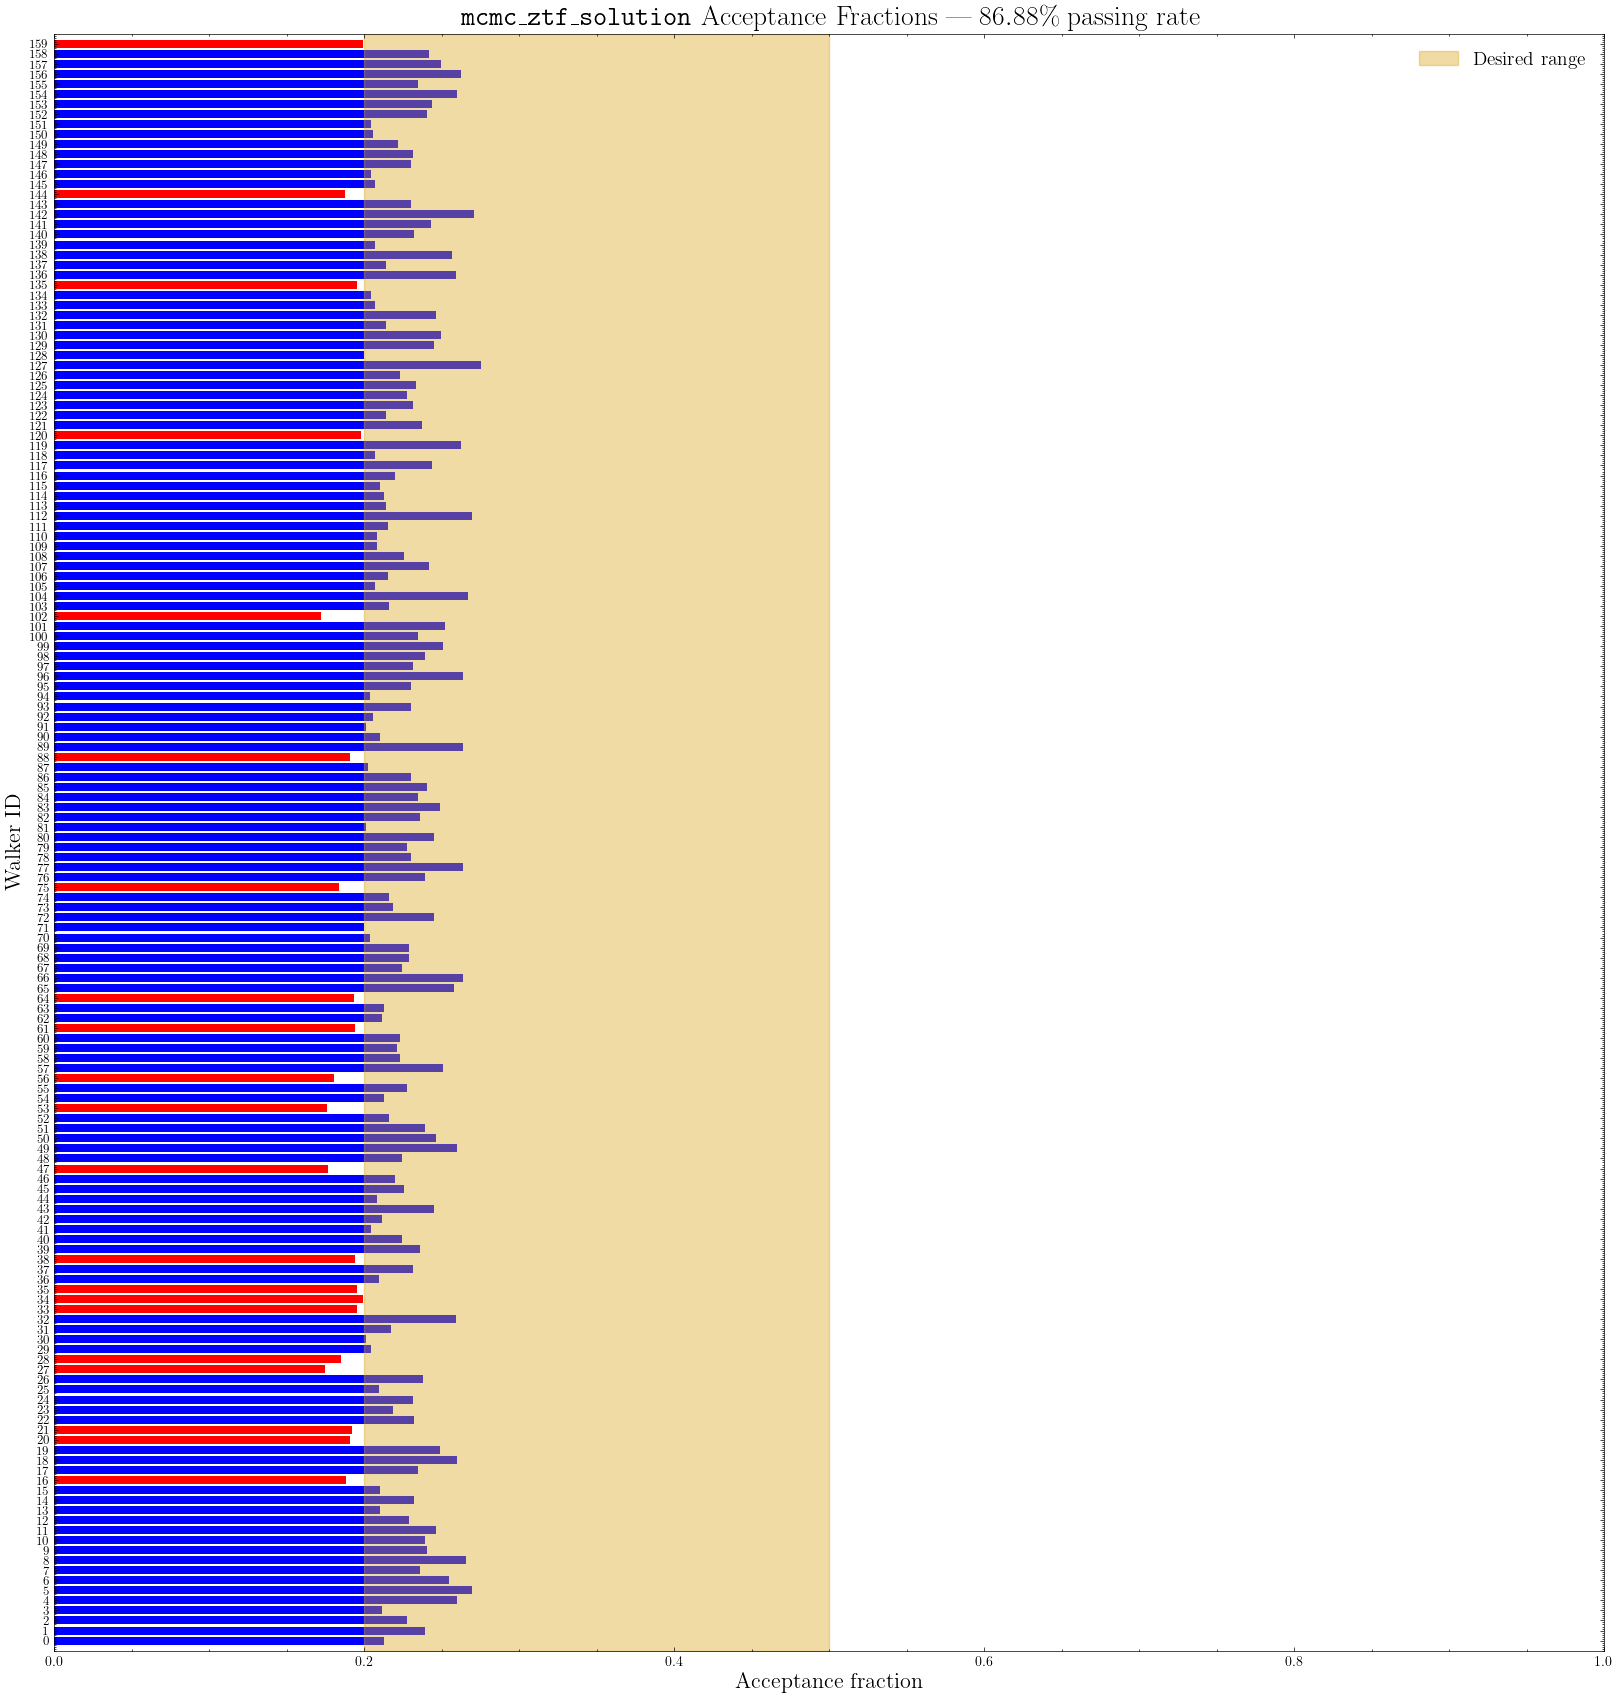
\includegraphics[scale=0.41]{Metodologia/Secciones/ModeloComputacional/Figures/Figura MCMC ZTF Acceptance Fractions.png}
	\caption{Fracción de pasos aceptados (eje \code{x}) para cada caminador (eje
	\code{y}) en el muestreo después de 865 iteraciones. El rango ideal de 0.2 a
	0.5 está marcado por la región amarilla. Aquellos caminadores que no estén
	dentro de este rango están resaltados por barras rojas.}
	\label{figuraFraccionPasosAceptados}
\end{figure}

% TODO: revisa titulo
% TODO: actualiza con últimos resultados
\subsection{Resultados - Funciones de Densidad de Probabilidad a Posteriori}

Las funciones de densidad de probabilidad (PDFs por sus siglas en inglés) se
pueden revisar tanto a lo largo del proceso utilizando los archivos de progreso,
como hasta el final que haya terminado de correr el número de iteraciones
configuradas en el resolvedor. Utilizando la distribución de las muestras en la
cadena se puede determinar las incertidumbres de cada parámetro y al mismo
tiempo inspeccionar de manera visual las correlaciones que existen entre
diferentes parámetros. La \reffigure{figuraMcmcZtfResultadosPrimarios} muestra
estas distribuciones.

% TODO: actualiza con últimos resultados y número iteraciones
\begin{figure}[!ht]
	\centering
	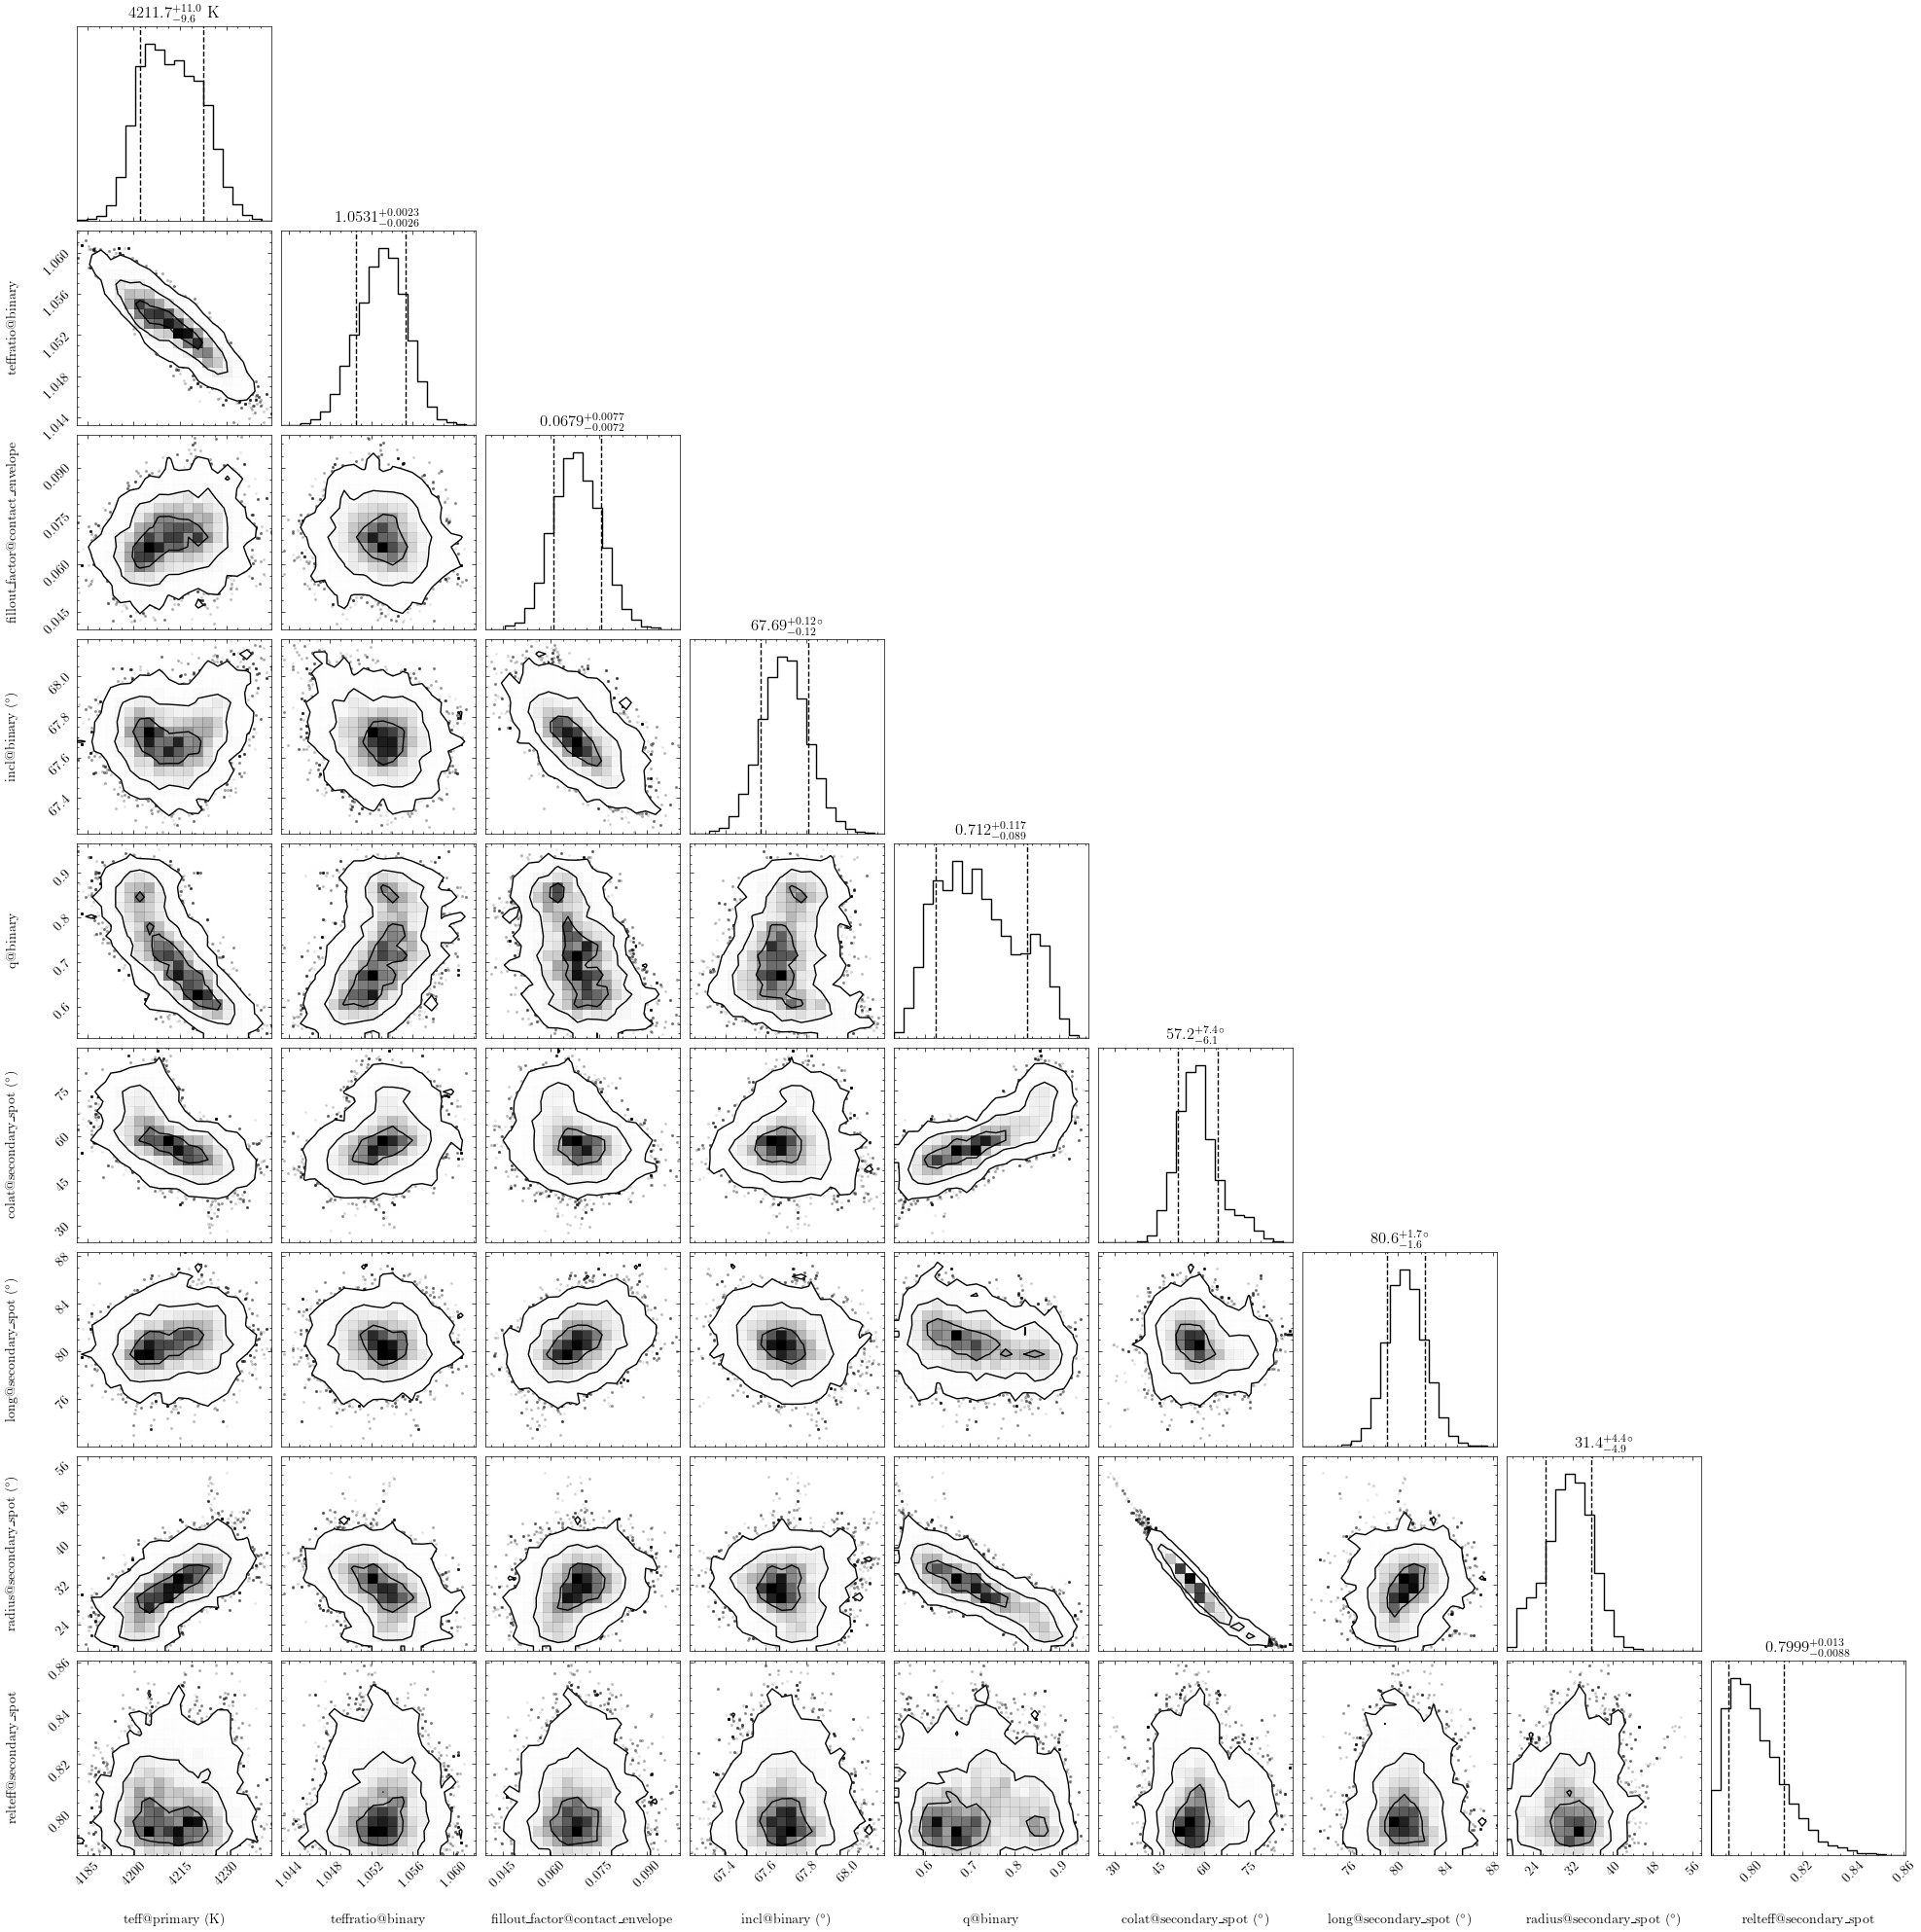
\includegraphics[scale=0.32]{Metodologia/Secciones/ModeloComputacional/Figures/Figura MCMC ZTF Resultados.png}
	\caption{Gráfica mostrando las muestras en la cadena después de 865
	iteraciones, marginalizando sobre la luminosidad de la pasabanda ZTF:g en la
	muestra. Los parámetros que se restringen mayormente por una curva
	fotométrica (la razón de temperaturas $T_2/T_1$ y la inclinación $i$)
	muestran una forma Gaussiana de la cual se puede obtener incertidumbres
	adecuadamente. La temperatura relativa de la mancha estelar \code{relteff}
	muestra una forma Gaussiana sesgada. Las correlaciones más significativas se
	pueden apreciar en esta figura; $T_2/T_1$\textemdash $T_1$ y
	$\mathrm{long}_{\mathrm{spot}}$\textemdash $T_{\mathrm{spot}}/T_2$ muestran
	una correlación aproximadamente lineal.}
	\label{figuraMcmcZtfResultadosPrimarios}
\end{figure}

La luminosidad se incluyó como un parámetro de molestia, el cual afecta el
modelo sintético resultante, pero no es un parámetro que nos interese medir.
Para los parámetros de interés se marginaliza (integra) sobre todos los
parámetros de molestia, incluyéndolos como parámetros que muestrear. La figura
completa incluyendo la luminosidad de pasabanda de ZTF:g se puede ver en el
apéndice en la \reffigure{figuraPhoebeMcmcResultadosCompletos}. Todas las
distribuciones posteriores en la cadena muestran una forma asimétrica, algunas
más pronunciadas que otras. PHOEBE reporta el valor promedio obtenido en la
muestra y 2 intervalos de confianza, los cuales se reportan en la
\reftable{tablaMcmcResultadosIncertidumbres}.

% TODO: actualiza con número de iteraciones
{\renewcommand{\arraystretch}{1.5}%
\begin{table}[!ht]
	\centering
	\begin{tabular}{|P{3cm}|P{4cm}|}
		\hline
		% \rowcolor{blue}
		\thead{Parámetro}                        & \thead{Valor} \\
		\hline
		$T_{ 1 }$ & $4211.7^{ +11.0 }_{ -9.6 } ~\mathrm{K}$ \\
		\hline 
		$T_2 / T_1 $ & $1.0531^{ +0.0023 }_{ -0.0026 } \mathrm{}$ \\
		\hline 
		$f$ & $0.0679^{ +0.0077 }_{ -0.0072 } \mathrm{}$ \\
		\hline 
		$i_\mathrm{ orb }$ & $67.69^{ +0.12 }_{ -0.12 } \mathrm{{}^{\circ}}$ \\
		\hline 
		$q$ & $0.712^{ +0.117 }_{ -0.089 } \mathrm{}$ \\
		\hline 
		$\mathrm{ Lat }_{\mathrm{spot}}$ & $57.2^{ +7.4 }_{ -6.1 } \mathrm{{}^{\circ}}$ \\
		\hline 
		$\mathrm{ Lon }_{\mathrm{spot}}$ & $80.6^{ +1.7 }_{ -1.6 } \mathrm{{}^{\circ}}$ \\
		\hline 
		$\mathrm{ Radius }_{\mathrm{spot}}$ & $31.4^{ +4.4 }_{ -4.9 } \mathrm{{}^{\circ}}$ \\
		\hline 
		$T_{\mathrm{spot}} / T_2$ & $0.7999^{ +0.013 }_{ -0.0088 } \mathrm{}$ \\
		\hline 
	\end{tabular}
	\caption{Valores obtenidos de la cadena de Markov junto a sus incertidumbres
	asimétricas. Estos valores fueron calculados después de 955 iteraciones.}
	\label{tablaMcmcResultadosIncertidumbres}
\end{table}}

\subsection{Incertidumbres en el Modelo Hacia Adelante}

Utilizando las distribuciones posteriores es posible visualizar la dispersión en
el modelo sintético. Esto se hace con el parámetro \code{sample\_from} del
cómputo en uso, en el cual se puede especificar las distribuciones de las cuales
obtener muestras individuales, calculando un modelo hacia adelante de estos
valores obtenidos. En la \reffigure{figuraMcmcZtfModeloDispersionPosterior} se
puede apreciar la dispersión (en las regions oscurecidas) del modelo promedio,
el cual surge como resultado de las incertidumbres de cada parámetro.

% TODO: actualiza cuando corran más iteraciones
\begin{figure}[!ht]
	\centering
	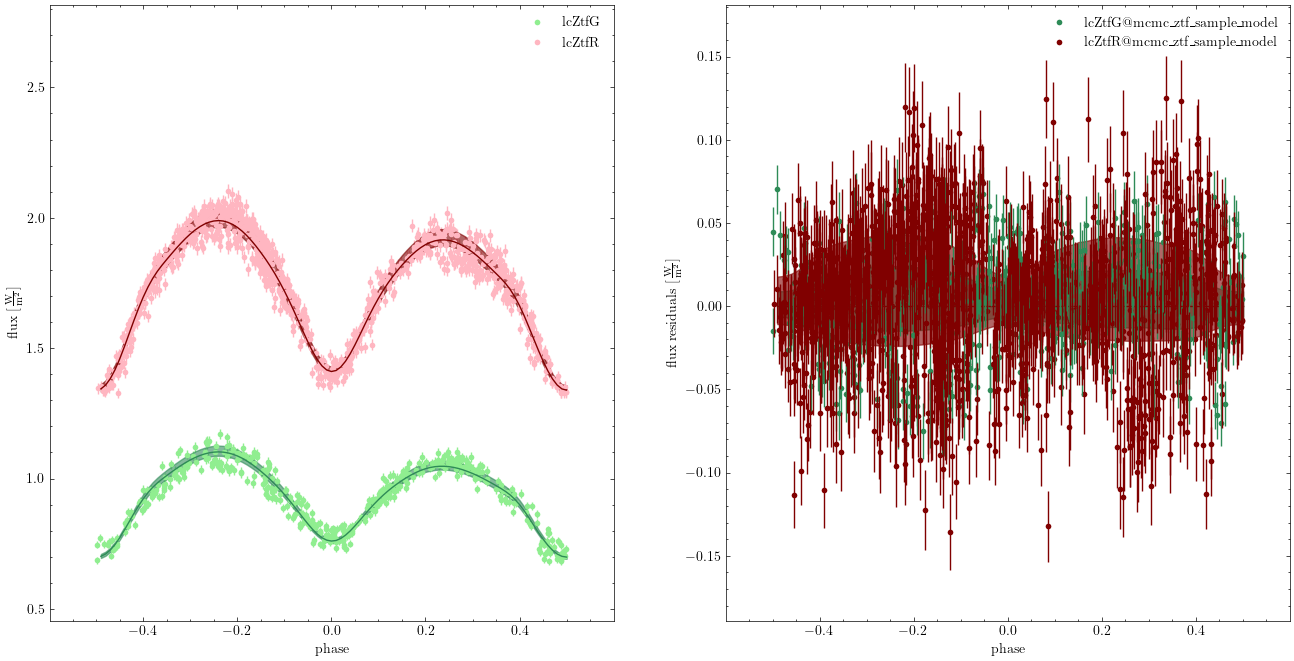
\includegraphics[scale=0.51]{Metodologia/Secciones/ModeloComputacional/Figures/Figura MCMC ZTF Modelo.png}
	\caption{Modelo sintético generado por PHOEBE utilizando muestras de la
	estimación de la distribución posterior obtenida mediante el proceso MCMC.
	Este modelo fue calculado con 100 muestras en total de las distribuciones
	posteriores.}
	\label{figuraMcmcZtfModeloDispersionPosterior}
\end{figure}

%%%%%%%%%%%%%%%%%%%%%%%%%%%%%%%%%%%%% Appendix
\appendix
\chapter{Gaia ADQL Encuestas} \label{apendice:gaiaAdql}

\section{DR2}
\begin{lstlisting}[ language=SQL,
	deletekeywords={IDENTITY},
	deletekeywords={[2]INT},
	morekeywords={clustered, Power},
	framesep=6pt,
	xleftmargin=6pt,
	framexleftmargin=6pt,
	frame=tb,
	framerule=0pt ]
SELECT *, 
	array_element(a0, 1) AS J2000_ra_prop,
	array_element(a0, 2) AS J2000_dec_prop,
	array_element(a0, 3) AS J2000_parallax_prop,
	array_element(a0, 4) AS J2000_pmra_prop,
	array_element(a0, 5) AS J2000_pmdec_prop,
	array_element(a0, 6) AS J2000_rv_prop, sdss_transform.g_sdss - sdss_transform.r_sdss AS g_r_sdss_color, sdss_transform.r_sdss - sdss_transform.i_sdss AS r_i_sdss_color
FROM (
	SELECT *,
		-0.13518 + 0.46245 * bp_rp + 0.2517 * Power(bp_rp , 2) - 0.021349 * Power(bp_rp , 3) + phot_g_mean_mag AS g_sdss,
		0.29676 - 0.64728 * bp_rp + 0.10174 * Power(bp_rp , 2) + phot_g_mean_mag AS i_sdss,
		0.12879 - 0.24662 * bp_rp + 0.027464 * Power(bp_rp , 2) +	0.049465 * Power (bp_rp , 3) + phot_g_mean_mag	AS r_sdss
	FROM (
		SELECT source_id, phot_variable_flag, bp_rp, phot_g_mean_mag, ra, dec, parallax, pmra, pmdec, radial_velocity AS rv, EPOCH_PROP(ra, dec, parallax, pmra, pmdec, radial_velocity, ref_epoch, 2000) AS a0
		FROM gaiadr2.gaia_source
	) as gdr2
	WHERE
		gdr2.phot_variable_flag = 'VARIABLE'
		AND gdr2.source_id IN (
			SELECT source_id 
			FROM external.gaiadr2_geometric_distance
		)
		AND gdr2.source_id NOT IN (
			SELECT source_id 
			FROM gaiadr2.sdssdr9_best_neighbour
		)
) AS sdss_transform
WHERE sdss_transform.g_sdss - sdss_transform.r_sdss < 0.7 AND sdss_transform.r_sdss - sdss_transform.i_sdss > 0.30
\end{lstlisting}

\section{DR3}
\begin{lstlisting}[ language=SQL,
	deletekeywords={IDENTITY},
	deletekeywords={[2]INT},
	morekeywords={clustered, Power},
	framesep=8pt,
	xleftmargin=8pt,
	framexleftmargin=8pt,
	frame=tb,
	framerule=0pt ]

SELECT
    *,
    array_element(a0, 1) AS J2000_ra_prop,
    array_element(a0, 2) AS J2000_dec_prop,
    array_element(a0, 3) AS J2000_parallax_prop,
    array_element(a0, 4) AS J2000_pmra_prop,
    array_element(a0, 5) AS J2000_pmdec_prop,
    array_element(a0, 6) AS J2000_rv_prop,
    sdss_transform.g_sdss - sdss_transform.r_sdss AS g_r_sdss_color,
    sdss_transform.r_sdss - sdss_transform.i_sdss AS r_i_sdss_color
FROM
    (
        SELECT
            *,
            -0.13518 + 0.46245 * bp_rp + 0.2517 * Power(bp_rp, 2) - 0.021349 * Power(bp_rp, 3) + phot_g_mean_mag AS g_sdss,
            0.29676 - 0.64728 * bp_rp + 0.10174 * Power(bp_rp, 2) + phot_g_mean_mag AS i_sdss,
            0.12879 - 0.24662 * bp_rp + 0.027464 * Power(bp_rp, 2) + 0.049465 * Power (bp_rp, 3) + phot_g_mean_mag AS r_sdss
        FROM
            (
                SELECT *, EPOCH_PROP(ra, dec, parallax, pmra, pmdec, radial_velocity, ref_epoch, 2000) AS a0
                FROM gaiadr3.gaia_source
            ) as gdr3
        WHERE
            gdr3.phot_variable_flag = 'VARIABLE'
            AND gdr3.source_id NOT IN (
                SELECT source_id FROM gaiadr3.sdssdr13_best_neighbour
            )
    ) AS sdss_transform
WHERE
    sdss_transform.g_sdss - sdss_transform.r_sdss < 0.7
    AND sdss_transform.r_sdss - sdss_transform.i_sdss > 0.30

\end{lstlisting}
%-------------------------------------REFERENCES
\chapter*{Agradecimientos}
This work has made use of data from the European Space Agency (ESA) mission {\it
        Gaia} (\url{https://www.cosmos.esa.int/gaia}), processed by the Gaia Data
Processing and Analysis Consortium (DPAC,
\url{https://www.cosmos.esa.int/web/gaia/dpac/consortium}). Funding for the DPAC
has been provided by national institutions, in particular the institutions
participating in the {\it Gaia} Multilateral Agreement.

This research made use of Astropy,\footnote{\url{http://www.astropy.org}} a
community-developed core Python package for Astronomy \autocite{astropy}.

This research has made use of the SIMBAD database, operated at CDS, Strasbourg, France.

This research made use of ccdproc, an Astropy package for
image reduction \autocite{ccdproc241}.
\clearpage

% \bibliography{ref}
\printbibliography

\end{document}
